%*************************************************************************************************************
% PREAMBLE STUFF
%*************************************************************************************************************
% Instead of inserting my \usepackage and defined commands here, I keep them in a separate file
\include{myPreamble}

%*************************************************************************************************************
% INCLUDE ONLY
%*************************************************************************************************************
% Use if you want to include only certain parts of the document, example \includeonly{introduction}
% in order to speed up compile time when you're focussing on some particular part.
%\includeonly{}


%*************************************************************************************************************
% DOCUMENT
%*************************************************************************************************************
\newcommand{\zrms}{z_{\rm rms}}
\newcommand{\zeff}{z_{\rm rms,eff}}
\renewcommand{\thepage}{}
%\newcommand{\last_page_of_biblio}{\def \last_page_number \numpages}
%\newcommand{\stitch_to_last_chapter}{\setcounter{page}{\last_page_number}}

\begin{document}

%*************************************************************************************************************
% TITLE
%*************************************************************************************************************

\title{Nature or Nurture? Collisionless Evolution of Galactic Disc-Halo Systems}

\author{J S Bauer}

\dept{Department of Physics}
\degree{Doctor of Philosophy}

% OPTIONAL HERE
% ~~~~~~~~~~~~~
% \submitdate{month year in which submitted to GPO}
%        - date LaTeX'd if omitted
% \copyrightyear{ear degree conferred}
%        - year LaTeX'd if omitted
% \figurespagetrue or \figurespagefalse
%        - produce or don't produce a List of Figures page (true by default)
% \tablespagetrue or \tablespagefalse
%        - produce or don't produce a List of Tables page (true by default)

\beforepreface

% Adding single spacing so abstract and table of contents is single spaced.

\begin{center}
\vspace*{\stretch{1}}
\noindent To Mom and Dad. Thank you for supporting me when I have been hard to support.

-- Your Loving Son
\vspace*{\stretch{1}}
\end{center}

\clearpage 

%{
%\noindent }%*************************************************************************************************************
% ABSTRACT
%*************************************************************************************************************

\prefacesection{Abstract}

In this thesis, we develop and apply a novel algorithm to understand 
the evolution of stellar discs in $\Lambda$CDM cosmological haloes.
Three main scientific areas are addressed: the effects of evolving stellar
discs on their host haloes, understanding bar formation in cosmological settings,
and the formation of vertical disc structure in response to the host halo.

First, we find that the presence of central concentrations of baryons in dark 
matter haloes enhances adiabatic contraction causes an overall modest 
reduction in substructure. Additionally, the detailed evolution of stellar discs 
is important for the inner halo density distribution. However,
properties of the halo such as the subhalo mass function are broadly unaffected
by the evolution of a realistic stellar disc.


Next, we find that stellar bars invariably form in Milky Way-like galaxies. The 
strength of these bars is less dependent on properties like the dynamical
temperature of the disc in a cosmological setting. Instead, the disc thickness
plays a leading role in determining the overall bar strength. Our discs
undergo notable buckling events, yielding present-day pseudobulge-disc-halo
systems. We show that these are qualitatively similar to the observed Milky Way.

Finally, we show that a wide variety of vertical structure forms when 
stellar discs are embedded in cosmological haloes. We further show that through
a variety of mechanisms, similar vertical structure is excited. By examining
twelve simulations of discs in cosmological haloes, we show that the Sgr dSph
need not be as massive as $10^{11}\,M_\odot$ to be consistent with observed
vertical structure in the Milky Way. In fact, the recent buckling of the Milky Way's
bar and its present interaction with the LMC are more likely culprits for some of
the observed structure in the Milky Way's thin disc.

%*************************************************************************************************************
% CO-AUTHORSHIP (if necessary)
%*************************************************************************************************************

%\prefacesection{Co-Authorship}



%*************************************************************************************************************
% STATEMENT OF ORIGINALITY (required CHEM, CISC, GEOL, MATH, PHYS (Ph.D. only))
%*************************************************************************************************************

\prefacesection{Statement of Originality}

The research presented in this thesis was completed under the supervision of Prof.
Lawrence M. Widrow at Queen’s University. All of the work presented here was done
by the author (Jacob S. Bauer) except where explicitly stated otherwise.

Chapter~\ref{ch:paper_i} contains a reproduction of a paper published in  Monthly Notices of the
Royal Astronomical Society as: Jacob S. Bauer, Lawrence M. Widrow, and Denis Erkal. Disc-halo interactions in $\Lambda$CDM. \textit{Monthly Notices of the Royal Astronomical Society}, 476:198-209,
2018. For this paper, I ran all of the simulations. The writing is mine with direct input from Lawrence M. Widrow and Denis Erkal. I performed all of the calculations. The analysis was handled primarily by me under the direction of Lawrence M. Widrow, with substantial input from Denis Erkal.

Chapter~\ref{ch:paper_ii} contains a reproduction of a paper published in  Monthly Notices of the
Royal Astronomical Society as: Jacob S. Bauer and Lawrence M. Widrow. Can stellar discs in a cosmological setting avoid forming strong bars?. \textit{Monthly Notices of the Royal Astronomical Society}, 476:523-537,
2019. For this paper, I ran all of the simulations. The writing is mine with direct input from Lawrence M. Widrow. I performed all of the calculations, except the one in \S2.3 which was performed by Lawrence M. Widrow. Figures 2-4 were also the work of Lawrence M. Widrow. The analysis was handled primarily by me under the direction of Lawrence M. Widrow.

Chapter~\ref{ch:paper_iii} contains a draft of a paper in preparation to be submitted to Monthly Notices of the Royal Astronomical Society. The working title for the paper is ``Vertical Structure and Kicked-Up Stars in $\Lambda$CDM Galaxies". For this work, I performed all of the simulations and writing. The analysis was handled primarily by me under the direction of Lawrence M. Widrow.

%*************************************************************************************************************
% ACKNOWLEDGEMENTS
%*************************************************************************************************************


\prefacesection{Acknowledgments}

As I reach the end of this chapter of my life, I know that I did not reach this milestone unassisted. Here, I recognize those who have helped me in this accomplishment.

I want to acknowledge, first and foremost, the amazing supervision I received from Larry Widrow. His careful, unyielding approach to scientific research has not only shown me how to be a better scientist, but a more conscientious communicator. I am immensely grateful for the opportunity to work with him, and for the years of guidance that will serve me well for the rest of my life.

In addition to Larry, I want to acknowledge my other mentors, Heidi Newberg and Denis Erkal. Through my work with each of them, I learned how to evaluate myself more honestly, both professionally and personally. I am grateful that through my work with my mentors, I learned to be simultaneously self-critical and able to forgive myself for mistakes. Without Heidi's and Denis' guidance, I would not have been able to finish this work.

To all of the other faculty members and Department staff, I am tremendously grateful for your contributions to me personally, and to the program as a whole. I am proud of my friends and colleagues at Queen's, and it is through your hard work that this positive academic environment exists. I wish you all the best.

I am grateful for the years of friendship with my fellow astronomy graduate students. In their own ways, they have all kept me mostly sane for 4 years. I would not have been able to persevere without their support. Although they did not succeed in turning me into a Canadian, they did manage to make me grow a beard. I look forward to many more years of friendship.

I want to acknowledge my wonderful family for their support. Mom and Dad have been my biggest supporters through the ups and downs, and this thesis is as much their accomplishment as it is mine. 

I am grateful to Rachel Peckman, Chris Weir, and Taylor Weir for our lasting friendships. In high school, Chris showed me that I was capable of pursuing science. Our adventures in Tech Club (RIP), our shenanigans at RPI (RIP), and subsequent friendship (not RIP) made me strive to be a better technologist and person.

Lastly, I want to acknowledge my partner, Alexis Hill. I can't wait to see what adventures life hold for us in Austin. I wouldn't want to be on this roller coaster called life with anyone else.



\singlespacing \afterpreface \doublespacing

\chapter*{List of Abreviations}
\begin{longtable}{ll} 
\hline
Abbreviation & Expansion \\ \hline
\textsc{AGAMA} & Action-based Galaxy Modelling Architecture \\
DF & Distribution Function \\
F(L)RW & Friedmann (Lema\^itre) Robertson Walker\\
GMC    & Giant Molecular Cloud\\
LAMOST & Large Sky Area Multi-Object Fiber Spectroscopic Telescope \\
LMC & Large Magellanic Cloud\\
M31 & Messier object 31 (Andromeda) \\
M33 & Messier object 33\\
NFW & Navarro-Frenk-White\\
RAVE & Radial Velocity Experiment \\
SDSS & Sloan Digital Sky Survey\\
Sgr dSph & Sagittarius Dwarf Spheroidal [Galaxy]\\
Sgr  & [The] Sagittarius [Stream]\\ 
SMC  & Small Magellanic Cloud  \\ \hline
\end{longtable}

\chapter*{List of Symbols}
\begin{longtable}{ll} 
\hline
Symbol/Unit & Meaning\\ \hline
Gyr & Gigayear; $10^9$ years\\
kg  & Kilogram; standard SI unit of mass\\
kpc & Kiloparsec; $10^3$ parsecs\\
m   & meter; standard SI unit of length\\
$M_\odot$ & Solar mass; approximately $2 \times 10^{30}$ kilograms\\
Mpc & Megaparsec; $10^6$ parsecs\\
Myr & Megayear; $10^6$ years\\
$O(f)$ & Big O notation; on the order of $f$ \\
pc  & parsec; approximately $3.1 \times 10^{16}$ meters\\
s   & second; standard SI unit of time\\
yr  & year; approximately $3.2 \times 10^7$ seconds\\ \hline
\end{longtable}
%*************************************************************************************************************
% MEATY CHAPTERS
%*************************************************************************************************************

%Testing my index\index{index} abilities.  And
%sub-entry\index{index!subentry} abilities.

% This command can be used to view the page layout for this document
% \layout

% Here, I'm tweaking how much space is put above and below floats.
% Comment out if you want the *purest* latex spacing.
%\setlength{\abovedisplayskip}{3pt plus1pt minus1pt}
%\setlength{\abovedisplayshortskip}{3pt plus1pt minus1pt}
%\setlength{\belowdisplayskip}{3pt plus1pt minus1pt}
%\setlength{\belowdisplayshortskip}{3pt plus1pt minus1pt}


% Include my chapter texts - kept separated to make editing easier.
%\include{Glossary}
\chapter{Introduction} \label{ch:introduction}
\newpage
%\section{Section}
%\subsection{SubSection}
%\subsubsection{SubSubSection}
%\paragraph{Paragraph}
%\subparagraph{SubParagraph}

\section{Perturbations to People}

Imagine you are standing on the corner of a busy Manhattan street. Every minute that passes shows the liveliness of a dynamic system, built up over many years. On an average block, there are approximately 28,154 people in the surrounding square kilometer, and a total of 1.7 million people on the island \citep{manhattan_population_density}. In contrast, a mere 300 years ago, the population was more disperse, and numbered in the thousands \citep{history_of_nyc}. Collections of thousands of people, initially spread out, came together to form a massive, dynamic ecosystem that represents an epicentre of modern human innovation and industry. Manhattan is not unique; cities across the world did not appear overnight, but were constructed hierarchically. It is in a similar fashion that modern astrophysics believes our Milky Way, and all massive galaxies formed with stars and gas as their building blocks.

We believe that the Universe began with a period of rapid inflation, and that in the process of this inflation, pockets of the Universe emerged more dense than other regions. This is revealed to us through observations of the cosmic microwave background (CMB). The CMB is a portrait of the Universe when it was last opaque; before electrons, neutrons, and protons combined to form the first atoms. It shows temperature fluctuations, like small population overdensities, that would eventually become cosmic cities.  While many physicists marvel at the physics that happens in these first moments of time, there is another story of how cosmic villages come together to form cities. This is the story of how tiny perturbations evolve to the structures astronomers see today.

When we look at the CMB, we are seeing the temperature distribution of matter through the radiation of baryonic matter, the matter that interacts with light. There is strong observational evidence to suggest that a large fraction of the matter present at this epoch is not interacting with light. This evidence is found in the power spectrum of the CMB, a function that describes the distribution of scales of the perturbations in the CMB \citep{transfer_fn}. 

This dark matter appears to be present in the current epoch. Evidence of dark matter in modern-day galaxy clusters was first observed by \citet{zwicky_1933}, who inferred that the mass of the Coma Cluster needed to be approximately ten times higher than observed to explain the motions of the constituent galaxies. A convincing case for dark matter in individual galaxies was presented by \citet{rubin_1980}, who show that the rotational speeds of stars in the disks of galaxies were too high to be explained by observed mass.

Based on enormous observational evidence, the dark matter component of the Universe appears to be substantial. If the results from the Planck satellite are taken as truth, then dark matter comprises around 84\% of all matter in the Universe \citep{planck_2018}. Dark matter influences the evolution of galaxies not only because it is not subject to radiation-based interactions, but also because it is most of what there is. Dark matter is the glue that holds galaxies together.  

Although dark matter makes up 84\% of the matter, matter only makes up 31.5\% of the present day Universe's total energy density. The remainder contains a modest contribution from radiation, but the bulk is comprised of unaccounted dark energy \citep{kolb_turner,dodelson, BT}. Dark energy, whatever it is, is responsible for the accelerating expansion of the Universe, something we first learned from from observations of Type 1a supernova \citep{reiss_1998,perlmutter_1999}. Modern cosmology is a struggle between the competing forces of dark matter and dark energy, and both have implications for the local dynamics in the Universe.

A model of the Universe one might consider is one comprised of cold dark matter, that is dark matter which is massive and slow, and one which has dark energy, described on large scales by a single parameter, $\Lambda$. This paradigm is called $\Lambda$CDM and is the prevailing model in the astronomy community. The model has been enormously successful in explaining observations, including the CMB power spectrum. While there remain open problems with $\Lambda$CDM, it appears to predict many properties on Galactic and extragalactic scales correctly \citep{kolb_turner,dodelson, BT}. Proposals to modify $\Lambda$CDM tend to present only slight variations on the model, such as allowing for self interacting dark matter (SIDM).
\begin{figure}
	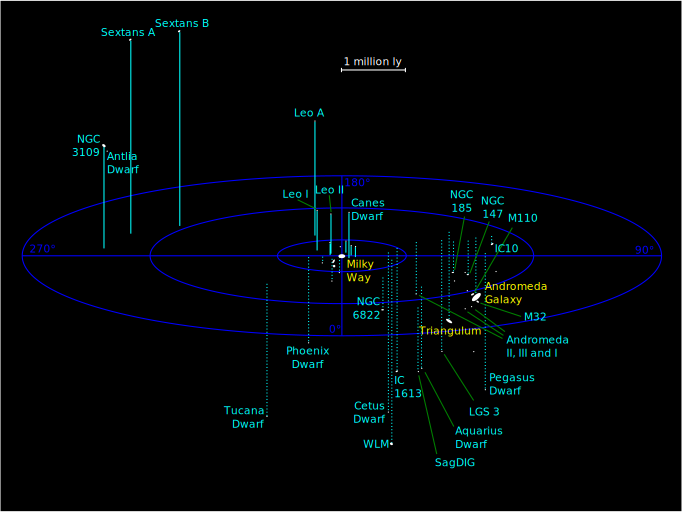
\includegraphics[width=\textwidth]{../figures/local_group}
	\caption{A map of the Local Group obtained per the license in \citet{local_group_map}.}\label{fig:local_group}
\end{figure}


\subsection{The Story of the Milky Way}
Taking $\Lambda$CDM as the ground truth, we can begin to understand how galaxies evolved from tiny villages. Dark matter, which does not interact through any force but gravity, retains a perturbed structure after inflation. The density perturbations collapse, forming potential wells of dark matter \citep{taylor_2011}. The baryons, interacting through baryon acoustic oscillations (BOA), are delayed in falling into the potential wells made by the dark matter. As the baryons fall into the centers of the potential wells over time, the cores of the dark matter distributions, comprised of spheroidal units called halos, contract. After infall into a dark matter halo, the baryons cool to the point where stars are able to form. This is how the first galaxies formed.

Over time, galaxies begin to shift away from the linear mapping between perturbation and galaxy. Their forces on each other start to matter locally, and galaxies begin to merge hierarchically. Collections of galaxies form, sometimes massive clusters of $10^{15}$ solar masses. Other times, groups with a couple massive galaxies become host to many smaller galaxies called subhalos. Other galaxies belong to no group or cluster, and exist in the expansive void between clusters. Dark energy continues to pull the Universe apart, while locally galaxies are kept together by dark matter. Merging of galaxies continues on local scales as larger galaxies become larger, bringing us to today.

We live in a spiral galaxy of approximately $10^{12}$ solar masses (dark matter + baryons), in a group with another galaxy, M31 (Andromeda), which has a roughly similar mass. Our Local Group (Fig. \ref{fig:local_group}), as it is called, is comprised of many smaller galaxies. In our Milky Way's halo, for instance, a merger is beginning between the Milky Way and the Large and Small Magellanic Clouds (LMC/SMC), shown in the third quadrant of the inner circle around the Milky Way in Fig. \ref{fig:local_group}. The SMC/LMC systems total approximately 10-20\% of the Milky Way's mass in total \citep{erkal_lmc}. Most of our subhalos are not nearly this massive, although they number in the hundreds. The picture painted of the Local Group is that of M31 and the Milky Way devouring smaller galaxies. Of course, this will have a substantial impact on the evolution of the stars in the Milky Way, and is the crux of this thesis. By studying the Milky Way's local environment, we can hope to understand the interactions dark matter has on baryons, and perhaps infer something about how dark matter is distributed in our Galaxy.

%...the current de facto standard being the Unified Modeling Language
%(UML)~\cite{BRJ99}...

%\section{Problem}

%\section{Objective}

%\notesbox{Note:  These are the section headings that I decided to use.  Check out several
%recent theses to decide how you want to lay out your introduction (and conclusion) chapters.}


%\subsection{Hypothesis}

\section{Understanding $\Lambda$CDM with Galaxy Simulations}

Many of the hardest questions in Galactic astrophysics stem from the fact that dark matter is not directly observable. As an example, what is the underlying smooth distribution of dark mass? How many dark matter subhalos should the Milky Way have? What is the effect on large scales if we choose something other than $\Lambda$CDM? While these questions are not easily answerable by direct observation, we can complement indirect observations with a solid theoretical understanding to reach confident answers.

Simulations are the complementary theoretical understanding of galactic and extragalactic systems. When a simulation is performed, theoretical input is considered. This includes a model of cosmology, or a model of the galaxy, the nature of dark matter, etc. All of this knowledge is reduced to a fluid system which may be solved through numerical techniques on a computer.  

Over the last four decades, many tools have been developed to study the structure of the present day Universe. These tools have become increasingly sophisticated as computation power and algorithms research advance. One tool is an \textit{ab initio} cosmological simulation, which simulates the entire formation history of the Universe from some informed initial density field.  This initial density field is derived from the primordial power spectrum and early-Universe baryon physics, and a sample can be drawn and evolved with periodic boundary conditions \citep{music}. If done correctly, this creates a representative sample of many structures in a $\Lambda$CDM Universe. Halos evolving in these simulations feel the full effect of the completely simulated cosmological environment. Such simulations stand in contrast to isolated galaxy simulations, which seek to explain the detailed dynamics arising from generic effects in individual galaxies. These simulations start with a prescription for what an equilibrium galaxy looks like, and study the evolution of galaxies initialized from these prescriptions. While missing some critical cosmological physics, these simulations may be run at very high resolution.


When the results of a simulation are studied, we are studying the output of a given set of assumptions. In principle, this should allow us to evaluate whether or not cosmology is consistent with dynamics on a Galactic scale. $\Lambda$CDM has been tested in this way for decades, and we detail some global results in what follows. In particular, we focus on where simulations have shown discrepancies in cosmological theory.

We broadly commented on the hierarchical formation of galaxies. Over time, galaxies that merge with other galaxies should become well-mixed in the host halo. That is, there should be an underlying smooth distribution of mass in which all of the subhalos reside. A key prediction of $\Lambda$CDM is that this smooth distribution should have a universal density profile in the limit that dark matter dominates the Universe \citep{nfw}. Furthermore, the dark matter should have a density distribution somewhat resembling a squashed football, a spheroid flattened on two axes. Whether or not this picture holds observationally in real galaxies is an open problem. The density profile proposed by \citet{nfw} is cuspy at the center, whereas some observations are more consistent with a flatter central density \citep{de_blok_core_cusp}. Astronomers have dubbed this the Core-Cusp Problem. From simply running a dark matter only simulation, we can infer the relative significance that baryonic physics plays in the central part of galaxies from these observational inconsistencies.

Besides the Core-Cusp Problem in the inner parts of dark matter haloes, one thing that is clear is that $\Lambda$CDM halos should have many subhalos. As the general theory for the formation of galaxies goes, these subhalos were at one point independent perturbations that have since merged into the Milky Way's halo, and should have their own stellar and gas content. This means that we expect many massive subhalos to be directly observable. Another triumph of simulations is putting an actual number on how many subhalos we expect from $\Lambda$CDM. Surprisingly, far fewer subhalos are actually observed \citep{mooresubhalos, Klypin1999, springel2008}. This discrepancy has since been dubbed the Missing Satellite Problem, and is an open problem for $\Lambda$CDM and astronomy.


The Core-Cusp Problem and Missing Satellite Problem have received a lot of attention in the literature because of the potential problems they pose for theoretical cosmology. It is clear that to accurately recover the global properties of substructure on large scales, dark matter must be cold. Warm and hot dark matter models\footnote{Hot dark matter is comprised of matter moving at or near the speed of light (e.g. neutrinos), and warm dark matter is somewhere in between cold and hot dark matter.} simply do not yield substructure populations consistent with observations \citep[for example]{alternate_dm}. SIDM and fuzzy models, where the dark matter can interact on small scales, have been proposed as slight modifications to the $\Lambda$CDM paradigm, with some success \citep[for example]{hui_2017}. 

Despite the presence of alternate theories of cosmology, a large concerted effort has been made to understand discrepancies as a byproduct of baryonic physics.  Adequate explanation of halo and substructure response to stellar and gas content would mean that alternate cosmologies are not necessary to explain the Core-Cusp Problem and Missing Satellite Problem. Initially, \textit{ab initio} simulations included only dark matter, but have evolved over the last three decades to consider very sophisticated subgrid models of gas physics and star formation \citep{LucySPH,CenOstriker92,KatzSPH96,SpringelMultiphase03,Stinson2006}.  These simulations can be used to realize the galaxy formation predicted by current theories. State of the art unigrid (single resolution) cosmological simulations struggle to compete with the resolution attainable by isolated galaxy simulations \citep{Illustris,Eagle}, but they can still be used to make broad statements about consistency with $\Lambda$CDM. Broadly speaking, it is not clear at this stage whether or not apparent issues with $\Lambda$CDM can be resolved through these models, but they present a promising approach as computing power is sure to increase.

%Because of resolution factors, the goal of many of cosmology studies has shifted from studying galaxy dynamics to reproducing population statistics such as scaling relations.  As a consequence, problems which are at the interface of the complex cosmological environment and individual galaxy dynamics are still open.

All of the preceding is to say that simulations are an enormously valuable tool in understanding the broad predictions of cosmology on a Galactic scale. We have used them to uncover apparent inconsistencies in $\Lambda$CDM, and have a promising means within the paradigm to move forward in resolving these inconsistencies. All of the preceding discussion has focused on the complexity of the halo environment. Ultimately, we are looking for simulations to make observable predictions, and specifically signatures outside the Galactic halo that theory is correct.

\section{Dynamical Processes in a Chaotic Milky Way}

Since dark matter is not directly probable, we must use indirect methods to infer information about the halo. In addition to the dark matter halo, our Galaxy is composed of baryons in the form of a central spheroidal bulge, a thin gas disk, a thin stellar disk, and a more diffuse thick stellar disk. There is also a stellar component of the halo, which contains remnants of old mergers and star clusters known as globular clusters. This section is organized by talking about tidal disruption of subhalos in the Galactic halo, the dynamics of the central part of the Galaxy, and vertical structure in the Galactic disk. How the cosmological environment effects these observables is the bulk of this thesis, and we motivate here why these aspects are the subject of focus.

\subsection{Stellar Streams from Mergers}

In the hierarchical formation of galaxies, smaller galaxies merge with larger galaxies and become a part of the larger galaxy's halo. As subhalos become more a part of the host system, they experience tidal forces that stretch them apart. Dark matter and stellar material is stripped from these merging galaxies over time to form streams of tidal debris. In the long run, this debris will equlibrate with the stellar halo. It should be noted that the same effects apply to globular clusters too.

At the beginning of a merger event, the stellar debris left behind can detected. This is no easy task, and the first stream for which this accomplished was the debris of the Sagittarius Dwarf Spheroidal galaxy (Sgr dSph). The Sgr dSph was discovered by \citet{ibata_discovery}. The corresponding stream was later detected by \citet{newberg_2002} and \citet{majewski_2003}. 

These discoveries of debris associated with a merging dwarf galaxy kickstarted an onslaught of literature based on the detection of streams, and their potential uses in probing the Galactic potential. The general idea is that so long as streams approximately trace orbits in the halo, the correct Milky Way potential, dark matter and all, is the unique potential that reproduces these orbits. 

More streams have been discovered since then, and a few notable ones are the Orphan Stream \citep{grillmair_2006,belokurov_2007,newberg_2010}, remarkable for its apparent lack of progenitor, TriAnd, A13, and the Monoceros Ring. This is by no means a complete accounting of known stellar streams. Something on the order of more than a dozen streams are known to exist in the Milky Way alone \citep{sanders_binney_2013_a}. While streams alone have been useful in getting some broad constraints on the Galactic potential and geometry of the halo, complications arise from the fact that streams do not follow orbits exactly \citet{sanders_binney_2013_a} and the fact that the Milky Way potential is predicted from theory to be time dependent.

The orbits of streams are not the only way to learn about the Milky Way's dark matter halo. It is worth mentioning that there is the possibility of using the fine structure of stellar streams to learn more about the subhalo population in the halo.  Gaps form when subhalos pass through tidal streams, and this is one direction that is being explored for leveraging stellar stream data (e.g. \citet{erkal_2016_stream_gaps}).

%With the Sagittarius stream specifically, there 
\subsection{Response of the Galactic Disk to the Cosmological Environment}


We might also attempt to infer properties of the subhalo population through their effect on the Galactic disc.  It is believed that the affect of the Milky Way's substructure population can be observed as waves-like behaviour in the thin disc's vertical structure \citep{widrow_2012_sdss,carlin_2013_lamost, williams_2013_rave,xu_2015, carrillo_2018_rave}.  These waves can manifest as small corrugations in the Galactic disc, as global bending and breathing motions, or even as large warps in the Milky Way's gas  \citep{gasWarp} and stellar discs. It is worth noting that these observations are being confirmed in DR2 of the Gaia mission \citep[for example]{gaia_collab,bennet_2019_gaia}.

The Milky Way's massive subhalos are most likely inducing non-planar density patterns in the disc, and we would like to understand the nature of these patterns through simulation. Unfortunately, we need the high resolution of isolated galaxy simulations to study these effects, and the realism of an \textit{ab initio} Galactic halo.  This has motivated a long history of attempts to bridge the gap between {\it ab initio} cosmological simulations and those of isolated galaxies.  A particularly simple class of simulations involves the interaction of a disc
with a single satellite galaxy or dark matter subhalo.  For example \citet{kazantzidis2008} perform simulations in which a thin Milky Way-like disc is subjected to a series of encounters with a satellite.  The masses and orbital parameters of the satellites are motivated by substructure found in a halo appropriate to a Milky Way-like galaxy from a cosmological simulation.  Their simulation demonstrated that satellite encounters lead to general disc heating as well as distinctive disc features such as bars, spiral structure, flares, and rings.  \citet{purcell2011} model the response of the Milky Way to the gravitational effects of
the Sgr dSph by simulating disc-dwarf encounter for different choices of the Sgr progenitor's mass.  Their conclusion is that Sgr may have triggered the development the spiral structure seen today in the Milky Way.  This approach has gained considerable traction in the last couple years, with authors using single-satellite encounters to explain the existence of low-latitude streams and other vertical structure in the Milky Way's disc \citep[for example]{widrow_2014, dlv_2015, donghia_2016, laporte_2016, laporte_2018}. One particularly interesting feature arising from these works is that stars may occasionally be kicked out of the galactic disc to form kicked-up disc populations \citep{johnston_kud_review, laporte_2019_feathers}. Such populations may explain low-latitude Milky Way structures, and possibly kinematic data of M31 \citep{dorman_2013_m31}.

% Say something about KUD since you will focus on it. One interesting feature... Which might explain MW M31

Of course, the disc of the Milky Way lives within a population of satellite galaxies and, quite possibly, pure dark matter subhalos, and single-satellite encounters do not describe the complexity of the cosmological environment \citep{Klypin1999,mooresubhalos,springel2008}.  With this in mind \citet{Font2001} simulated the evolution of an isolated disc-bulge-halo model where the halo was populated by several hundred subhalos.  They concluded that that substructure played only a minor role in heating the disc, a result that would seem in conflict with those of the \citet{kazantzidis2008} that would come later.  Numerical simulations by \citet{gauthier2006, dubinski2008} sheds some light on this discrepancy.  In these simulations, 10\% of the the halo mass in an isolated disc-bulge-halo system is replaced by subhalos with a mass distribution motivated by the cosmological studies of \citet{gao2004}.  In the \citet{gauthier2006} simulation, little disc heating occurs during the first 5 Gyr, at which point satellite interactions provoke the formation of a strong bar, which in turn leads to significant heating.  Not surprisingly, when the experiment is repeated with different initial conditions for the satellites the timing of bar formation can vary.  These experiments also suggest that a large fraction of the mass initially in subhalos is tidally stripped leaving behind a complex system of tidal debris.

The aforementioned simulations, although more realistic than single-satellite encounters, have three main problems.  First, they don't allow for halo triaxiality.  Secondly, the disc is initialized at its present-day mass whereas real stellar discs form over several Gyr.  Finally, the subhalo populations are inserted into the halo by hand.  While the mass and spatial distributions of the subhalos are motivated by cosmological simulations, they may not capture important properties of realistic halos. This has historically been solved by modifying a traditional \textit{ab initio} simulation. The zoom-in technique (a Monte Carlo adaptive mesh) is used to study the evolution of a disc in a single halo at high resolution.  This is accomplished by resampling the initial conditions at a sequence of higher resolutions after identifying an area of interest. With sufficiently realistic feedback, impressively realistic results can be obtained. For instance, \citet{gomez_2017} presented a study of vertical structure in such simulations. In these simulations, the authors were able to look at several Milky Way-like galaxies in a variety of environments at resolutions that rival isolated galaxy simulations. These realistic studies have opened the door to a wide variety of questions pertaining to the Milky Way's interaction with the cosmological environment.

\section{Disk Insertion Techniques for Cosmology}

While highly realistic, the \textit{ab initio} zoom-in approach still suffers from the inability to fine-tune galaxy dynamics in the same halo to perform a truly systematic study. In an effort to address these particular shortcomings, several groups have attempted to grow a stellar disc in a cosmological halo.  

% Should add a footnote about redshift

The general idea for the modification is to divide a dark-matter-only (DMO) zoom-in simulation into three phases.  During the first, a cosmological simulation of a region of interest is run, and a halo is identified for study.  A rigid disc potential is then slowly grown in this halo, allowing the halo particles to respond adiabatically to its time-varying potential.  Finally, the rigid disc is replaced by live particles and the final phase of the simulation proceeds with live disc and halo particles.  \citet{debuhr_2012} use this scheme to introduce stellar discs into dark matter halos from the Aquarius Project \citep{springel2008}.  They add a rigid disc potential at redshift $z=1.3$ with a mass parameter for the disc that grows linearly with the scale factor until $z=1$ when it reaches its final value.  The disc potential is initially centered on the potential minimum of the halo and oriented so that its symmetry axis points along either the minor or major axis of the halo.  During the rigid disc phase, the centre of the potential moves due to its interaction with the halo (Newton's 3rd law) so that linear momentum is conserved.  However, the orientation of the disc is held fixed and therefore angular momentum isn't.  To initialize the live disc, \citet{debuhr_2012} approximate the halo potential as a flattened logarithmic potential and then determine the disc distribution function by solving the Jeans equations in axisymmetry. 

A number of refinements to this scheme were introduced by \citet{ys_2015}.  In particular, they use the GALIC code to initialize the live disc \citet{YurinSpringelGalic}.  This code aims to find a stationary solution to the collisionless Boltzmann equation by adjusting the initial particle velocities so as to minimize a certain merit function.  In \citet{ys_2015} the initial disc distribution function was assumed to depend on two integrals of motion, the energy $E$ and angular momentum $L_z$.  Consistency then required that they use an axisymmetrized approximation to the halo potential.

\citet{bauer2018a} improved on the scheme even further by increasing the realism of the growth phase by modelling the disc as a rigid body. The results they found were qualitatively similar to \citet{debuhr_2012} and \citet{ys_2015}  in terms of disc dynamics. The live phase was also improved by using the \textsc{GalactICS} code which actually samples a three-integral DF. It is using this tool that this thesis is constructed upon.


\section{Organization of Thesis}

The thesis is organized in the following manner. In Chapter~\ref{ch:background}, we reduce the necessary theoretical background to understand this work to a succinct summary. Following this, in Chapter~\ref{ch:paper_i}, we explore the first peer-reviewed paper on which this thesis is based. It outlines the disk insertion scheme and comments on how the dynamic nature of the Milky Way's stellar disk should affect its inner halo. Chapter~\ref{ch:implementation} is intended to clarify some implementation details of the algorithm in Chapter~\ref{ch:paper_i}. Chapter~\ref{ch:paper_ii} presents the second published paper which focuses on the question of how stable disks are against forming bars in a cosmological setting. A final paper is presented in Chapter~\ref{ch:paper_iii}, where we look at how disks form vertical structure in a cosmological setting. We conclude with summaries and ideas for future work in Chapter~\ref{ch:conclusion}.

\bibliographystyle{apalike}
\bibliography{bibliography_introduction}
\chapter{A Dynamical Recipe for Cosmological Disks}\label{ch:Background}

\section{Physical Motivation of Modeling}

\section{Time Evolution of Collisionless Systems}
\subsection{The Collisionless Boltzmann Equation}
\subsection{Numerical Solutions}

\section{Phase Space, Equilibrium, and Initial Conditions}
\subsection{Jeans Modeling}
\subsection{DF-based Models and the Strong Jeans Theorem}
\subsection{Action-Angle Variables}
\subsection{DFs as Functions of Actions}

\section{Simulation Analysis: Paradigms and Tools}
\subsection{WKB Wave Analysis}
\subsection{Time Series Filtering}
\subsection{MCMC}

\section{Cosmology and Implications for Galaxy Studies}
\subsection{Basic FRW Cosmology}
\subsection{Extension of Numerical Methods}
\subsection{Sampling Initial Conditions for Cosmological Simulations}
\subsection{Cosmological Substructure and Halo Triaxiality}
\subsection{Identifying Substructure in Simulations}


\chapter{A Method for Studying Discs in Cosmological Haloes} \label{ch:paper_i}
\textbf{This chapter contains a reproduction of a paper published in  Monthly Notices of the
Royal Astronomical Society as: Jacob S. Bauer, Lawrence M. Widrow, and Denis Erkal. Disc-halo interactions in $\Lambda$CDM. \textit{Monthly Notices of the Royal Astronomical Society}, 476:198-209,
2018.}
\newpage
\section{Abstract}

We present a new method for embedding a stellar disc in a
cosmological dark matter halo and provide a worked example from a
$\Lambda$CDM zoom-in simulation.  The disc is inserted into the halo
at a redshift $z=3$ as a zero-mass rigid body.  Its mass and size
are then increased adiabatically while its position, velocity, and
orientation are determined from rigid-body dynamics.  At $z=1$,
the rigid disc is replaced by an N-body disc whose particles sample
a three-integral distribution function (DF).  The simulation then
proceeds to $z=0$ with live disc and halo particles.  By comparison,
other methods assume one or more of the following: the
centre of the rigid disc during the growth phase is pinned to the
minimum of the halo potential,  the orientation of the rigid disc is
fixed,  or the live N-body disc is constructed from a two rather than
three-integral DF.  In general, the presence of a disc makes the halo
rounder, more centrally concentrated, and smoother, especially in
the innermost regions.  We find that methods in which the disc is
pinned to the minimum of the halo potential tend to overestimate the
amount of adiabatic contraction.  Additionally, the effect of
the disc on the subhalo distribution appears to be rather insensitive
to the disc insertion method.  The live disc in our simulation
develops a bar that is consistent with the bars seen in late-type
spiral galaxies. In addition, particles from the disc are
launched or ``kicked up'' to high galactic latitudes.

\section{Introduction}

The structure and evolution of galaxies are determined by the spectrum
of primordial density perturbations, the dynamics of stars and dark
matter, and baryonic physics.  Over the past two decades, there has
been a concerted effort to incorporate the latter into cosmological
simulations \citep[e.g.][]{katz1996feedback, springel2003feedback,
  stinson2006, RoskarDiskMisalignment, pakmorMHD, gomezwarps}.  While
these simulations have enhanced our understanding of galaxy formation,
their computational cost is high.  Adding to the challenge is the
complex and sub-grid nature of star formation, supernova feedback, and
other baryonic processes, which require {\it ad hoc} parametric
models.

In this work, we focus on the dynamics of disc galaxies.  Our goal is
to study the nature of disc-halo interactions where it is advantageous
to be able to control properties of the disc such as its mass, size,
and internal kinematics.  Such control is not possible in {\it ab
  initio} simulations.

Simulations of isolated disc galaxies provide an alternative arena to
study galactic structure and dynamics.  Moreover, many aspects of
disc-halo interactions can be understood by considering the
collisionless dynamics of stars and dark matter while ignoring gas
physics.  For example, simulations of stellar disc-bulge systems
embedded in dark haloes have proved indispensable in studies of bar
and spiral structure formation (See \citet{Sellwood2013} and
references therein).  These simulations typically begin with systems
that are in equilibrium, or nearly so.  For this reason, they usually
assume axisymmetric initial conditions, which are manifestly
artificial.  In short, discs do not come into existence as formed,
highly symmetric objects but rather build up through the combined
effects of gas accretion, star formation, and feedback
\citep{IllustrisFeedback, Eagle}.  Moreover, the haloes in which the
real discs reside are almost certainly triaxial and clumpy
\citep{NFW,mooresubhalos,Klypin1999}.

There now exists a long history of attempts to bridge the gap between
simulations of isolated disc-bulge-halo systems, with their pristine
initial conditions, and cosmological simulations.
\citet{kazantzidis2008}, for example, followed the evolution of a
Milky Way-like disc in its encounter with a series of satellites whose
properties were motivated by cosmological simulations.  They found
that the satellites ``heated'' the disc and prompted the formation of
a bar and spiral structure.  Along similar lines, \citet{purcell2011}
modeled the response of the Milky Way to the gravitational effects of
the Sagittarius dwarf galaxy (Sgr) by simulating disc-satellite
encounters for different choices of the satellite mass.  They
concluded that Sgr may have triggered the development of the spiral
structure seen in the Milky Way today. Continuing in this vein, \citet{laporte_et_al_2016} studied the
influence of the Large Magellanic Cloud and Sgr on the Milky Way disc and
found that they can create similar warps to what has been observed. The effect of a time-dependent triaxial halo
was investigated in \citet{hu_sijacki_2016} where they found it can trigger grand-design spiral
arms. 

Of course, the disc of the Milky Way lives within a population of
satellite galaxies and, quite possibly, pure dark matter subhaloes
\citep{mooresubhalos,Klypin1999}.  With this in mind \citet{Font2001}
simulated the evolution of an isolated disc-bulge-halo model where the
halo was populated by several hundred subhaloes.  They concluded that
that substructure played only a minor role in heating the disc, a
result that would seem at odds with those of \citet{kazantzidis2008}.
Numerical simulations by \citet{gauthier2006} and \citet{dubinski2008}
shed some light on this discrepancy.  In those simulations, 10\% of
the halo mass in an isolated disc-bulge-halo system was replaced by
subhaloes with a mass distribution motivated by the cosmological
studies of \citet{gao2004}.  \citet{gauthier2006} found that a modest
amount of disc heating occurred during the first 5 Gyr, at which point
satellite interactions prompted the formation of a bar, which in turn
heated the disc more significantly.  Not surprisingly, the timing of
bar formation varied from 1 Gyr to 10 Gyr when the experiment was
repeated with different initial conditions for the satellites.

The aforementioned simulations have several drawbacks.  First, most of them do
not allow for halo triaxiality.  Second, the disc is initialized at
its present-day mass whereas real discs form over several Gyr.
Finally, the subhaloes are inserted into the halo in an \textit{ad
  hoc} fashion.  Several attempts have been made to grow a stellar
disc in a cosmological halo in an effort to address these
shortcomings \citep{BerentzenShlosmanStellarDisks,DeBuhrStellarDisks, YurinSpringelStellarDisks}.  The general scheme proceeds in three stages.  During
the first stage, a cosmological simulation is run with pure dark
matter and a suitable halo is selected.  In the second, a rigid disc
potential is grown slowly in the desired halo, thus allowing the halo
particles to respond adiabatically to the disc's time-varying
potential.  In the third stage, the rigid disc is replaced by a live
one and the simulation proceeds with live disc and halo particles.

\citet{DeBuhrStellarDisks} used such a scheme to introduce stellar
discs into dark matter haloes from the Aquarius Project
\citep{springel2008}.  They added a rigid disc at a redshift $z=1.3$
with a mass parameter for the disc that grew linearly with the scale
factor from an initial value of zero to its final value at $z=1$.  The
disc was initially centered on the potential minimum of the halo and
oriented so that its symmetry axis pointed along either the minor or
major axis of the halo.  During the rigid disc phase, the motion of
the disc centre of mass was determined from Newton's 3rd law.
To initialize the live disc, \citet{DeBuhrStellarDisks} approximate
the halo potential as a flattened, axisymmetric logarithmic potential
and then determine the disc distribution function (DF) by solving the
Jeans equations.  

\citet{YurinSpringelStellarDisks} introduced a number of improvements
to this scheme.  Most notably, they use \textsc{galic} to initialize
the live disc \citep{YurinSpringelGalic}.  This code is based on an
iterative scheme for finding stationary solutions to the collisionless
Boltzmann equation.  The general idea for iterative codes is to begin with a set of
particles that has the desired spatial distribution and some initial
guess for the velocity distribution.  The velocities are then adjusted
so as to achieve stationarity, as measured by evolving the system and
computing a certain merit function.  In
\citet{YurinSpringelStellarDisks} the initial disc was assumed to be
axisymmetric with a DF that depended on two integrals of motion, the
energy, $E$, and angular momentum, $L_z$. One striking, if not puzzling,
result from this work is the propensity of the discs to form very
strong bars.  These bars are especially common in models without
bulges even in cases where the disc is submaximal.

In this paper, we introduce an improved scheme for inserting a live
disc in a cosmological halo.  In particular, the centre of mass {\it
  and} orientation of the rigid disc are determined by solving the
standard equations of rigid body dynamics.  Thus, our rigid disc can
undergo precession and nutation.  The angular and linear velocities of
the rigid disc at the end of the growth phase are incorporated into
the live disc initial conditions.  As in
\citet{YurinSpringelStellarDisks} we use an axisymmetric approximation
for the halo potential when constructing the disc DF.  However, our DF
is constructed from an analytic function of $E$, $L_z$, and the
vertical energy $E_z$, which is an approximate integral of motion used
in \textsc{galactics} \citep{DubinskiKuijkenRigidDisks,
  WPDGalactICSReference}.  By design, the disc DF yields a model whose
density has the exponential-${\rm sech}^2$ form.  And with a
three-integral DF, we have sufficient flexibility to model realistic
Milky Way-like discs.  As discussed below, the initial disc DF may be
crucial in understanding the formation of the bar.

As a demonstration of our method we grow a Milky Way-like disc in an approximately
$10^{12}\,h^{-1}\,M_\odot$ halo from a cosmological zoom-in
simulation.  We discuss both disc dynamics and the effect our disc has
on the population of subhaloes.  Discs have been invoked as a means of
depleting halo substructure and thus alleviating the Missing Satellite
Problem, which refers to the underabundance of observed Milky Way
satellites relative to the number of Cold Dark Matter subhaloes seen
in simulations \citep{mooresubhalos,Klypin1999}.  An earlier study by
\citet{DOhngiaSubstructureDepletion} found that when a disc potential
is grown in a Milky Way-size cosmological halo, the abundance of
substructure in the mass range $10^7\,M_\odot$ to $10^9\,M_\odot$ was
reduced by a factor of $2-3$.  Similar results were found by
\citet{Sawala2017} and \citet{GKSubhaloDepletion17}.

The organization of the paper is as follows.  In Section 2, we outline
our method for inserting a live disc into a cosmological simulation.
We also present results from a test-bed simulation where a disc is
inserted into an isolated flattened halo.  We next apply our method to
a cosmological zoom-in simulation.  In Section 3, we focus on disc dynamics
and find that the disc develops a bar, spiral structure and a warp.
In addition, disc-halo interactions appear to ``kick'' stars out of
the disc and into regions normally associated with the stellar halo.
In Section 4, we present our results for the spherically-averaged
density profile and shape of the dark matter halo as well as the
distribution of subhaloes.  Particular attention is paid to the
sensitivity of these results to the disc insertion scheme.  We
conclude in Section 5 with a summary and discuss possible applications
of this work.

\begin{table*}
\begin{tabular}{l l l l l l l}
\hline
 & DMO & MN & FO & RD & LD\\
\hline
$M_d \, (M_\odot)$ & -- & $7.2 \times 10^{10}$ & $7.2 \times 10^{10}$ & $7.2 \times 10^{10}$ & $7.2 \times 10^{10}$\\
$R_{d,0}$ (kpc) & -- & 3.7 & 3.7 & 3.7 & 3.7\\
$N_d$ & -- & -- & $10^6$& $10^6$ & $10^6$\\
$z_g$ & -- & 3.0 & 3.0 & 3.0 & --\\
$z_l$ & -- & 1.0 & 1.0 & 1.0 & 1.0\\
$N_r$ & 4096 & 4096 & 4096 & 4096 & 4096\\
$L_{box} (\text{ Mpc} \,h^{-1} )$ & 50  & 50 & 50 & 50 & 50\\
\hline
%$M_d$ & $7.2 \times 10^{10} M_\odot$\\
%$N_d$ & $10^6$\\
%$R_{d,0}$ & 3.7 kpc\\
%$N_{r}$ & $4096^3$
\end{tabular}\caption{A summary of the simulation parameters, as discussed in the text. $M_d$ is the final disk mass, $R_{d,0}$ is the final disk scale radius, $N_d$ is the number of particles used to simulate the disk, $z_g$ and $z_l$ are the redshifts when the disk beings to grow and when it becomes live (respectively), $N_r$ is the effective resolution in the zoom-in region, and $L_{box}$ is the comoving size of the box. } \label{tab:simparams}
\end{table*}

\section{Inserting a Stellar Disc into a Cosmological Halo}

In this section, we detail our method for inserting a live stellar
disc into a cosmological simulation.  We begin with an overview of our
approach and the five main simulations presented in this paper.  We
then describe some of the more technical aspects of the method.

\subsection{Overview of Simulation Set} \label{sec:sim_overview} 

Our simulations are performed with the N-body component of
\textsc{gadget-3}, which is an updated version of \textsc{gadget-2}
\citep{springel_2005}.  For the cosmological simulations, we implement
the zoom-in technique of \citet{KatzQuasarZoom} and
\citet{NavarroWhiteZoom}, broadly following the recommendations of
\cite{onorbe_etal_2014}, which allows us to achieve very high spatial
and mass resolution for a single halo while still accounting for the
effects of large-scale tidal fields. For the cosmological parameters, we
use the results from Planck 2013 \citep{planck_2014} with $h=0.679$, $\Omega_b = 0.0481$, 
$\Omega_0 = 0.306$, $\Omega_\Lambda = 0.694$, $\sigma_8 = 0.827$, and $n_s = 0.962$. 

We begin by simulating a $50\,h^{-1} {\rm Mpc}$ box with $N_r=512^3$ particles, where $N_r$ is the effective resolution, each with a mass 
of $\sim 7.9\times 10^{7}\,h^{-1} M_\odot$.  We identify a Milky Way-like
halo in the present-day snapshot, that is, a $\sim 10^{12}\,M_\odot$
halo which has experienced no major mergers since $z=1$ and which has
no haloes with $2 h^{-1}$ Mpc more than half the mass of the MW-analogue. We then run an
intermediate zoom-in simulation targeting all particles within 10
virial radii of the low resolution halo.  The initial conditions for
this simulation are generated with \textsc{music} \citep{music}, which
creates five nested regions from a coarse resolution of $N_r=128^3$ in the
outskirts to an effective $N_r=2048^3$ resolution in the targeted region.
After this simulation reaches $z=0$, we select all particles within
7.5 virial radii and regenerate initial conditions with one more level
of refinement, giving six nested zoom regions, where now, the highest
effective resolution is $N_r=4096^3$. Our final halo is composed of
approximately $10^7$ particles, each with a mass of
$1.54\times 10^5\,h^{-1} M_\odot$. The softening lengths were selected using
the criteria in \citet{power_et_al_2003} with a softening of $719$ comoving pc for the highest resolution 
particles in the final zoom-in simulation. We found that this repeated zoom-in technique
results in remarkably little contamination from coarse resolution
particles within the targeted halo, giving a clean region of size $1.9 h^{-1}$ Mpc at $z=0$.

The dark matter only (DMO) simulation not only serves as the basis for
four simulations with discs but also provides a control ``experiment''
for our study of the effect discs have on halo properties.  In each of
our disc simulations, the potential of a rigid disc is introduced at
the ``growing disc'' redshift $z_g$.  The mass parameter of the disc
is then increased linearly with the scale factor
$a = 1/\left (1+z\right )$ from zero to its final value $M_d$ at the
``live disc'' redshift $z_l$.  As described in
Sec.~\ref{sec:rigid_disks}, the radial and vertical scale lengths of
the disc are also increased between $z_g$ and $z_l$ to account for the
fact that discs grow in scale as well as mass while they are being
assembled.

In the first of our disc-halo simulations, dubbed MN, we introduce a
rigid Miyamoto-Nagai disc \citep{MiyamotoNagai}, whose gravitational
potential is given by

\begin{equation}
  \Phi\left (R,\,z\right ) = -\frac{G M_d} {\left (R^2 + \left(R_d +
    \left(z^2 + z_d^2 \right)^{1/2}\right)^{2}\right )^{1/2}}~.
\end{equation}

\noindent For this simulation, which was meant to mimic the scheme in
\citet{DOhngiaSubstructureDepletion}, we assume that the centre of the
disc tracks the minimum of the halo potential while the orientation of
the disc is fixed to be aligned with the $z$-axis of the simulation
box. Note that this is effectively a random direction for the halo.

In the remaining three disc simulations, we grow an
exponential-sech$^2$ rigid disc potential in our halo with mass and
scale-length parameters that grow in time.  For our fixed-orientation
(FO) simulation, the position and velocity of the disc's centre of
mass are determined from Newtonian dynamics while the spin axis of the
disc is initially aligned with the minor axis of the halo at $z = z_g$
and kept fixed in the simulation box frame thereafter.  In this
respect, the simulation is similar to the ones presented in
\citet{DeBuhrStellarDisks} and \citet{YurinSpringelStellarDisks}.  For
the rigid-disc (RD) simulation the disc's orientation, which is now a
function of time, is determined from Euler's rigid body equations.

In the MN, FO, and RD runs, we continue the simulation to the present
epoch ($z=0$) with the assumed rigid disc potential where the mass and
scale length parameters are held fixed and the position and
orientation are calculated as they were during the growth phase.  For
our final live disc (LD) simulation, we swap a live disc for the RD
disc at $z_l$.  Thus, the RD and LD simulations are identical prior to
$z_l$.  All of our discs have a final mass of
$M_d = 7.2 \times 10^{10} M_\odot$, a final scale radius of
$3.7\,{\rm kpc}$, and a final scale height of $0.44\, {\rm kpc}$. Our simulation
parameters can be found summarized in Table \ref{tab:simparams}.

\vspace{0.1in}
\subsection{Summary of Live Disc Insertion
  Scheme} \label{sec:method_outline}

The first step in our disc insertion scheme is to calculate an
axisymmetric approximation to the gravitational potential of the DMO
halo at $z=0$.  We do so using an expansion in Legendre polynomials as
described below.  We then generate a particle representation of a
stellar disc that is in equilibrium with this potential using the
\textsc{galactics} code
\citep{KGGalactICSReference,WPDGalactICSReference}.  Though
\textsc{galactics} allows one to generate the phase space coordinates
of the disc stars, at this stage, we only need the positions of the
stars, which we use to represent the ``rigid disc''.  At the $z_g$
snapshot, we incorporate the disc particles into the mass distribution
of the system with the disc centered on the potential minimum of the
halo.  We then rerun the simulation from $z_g$ to $z_l$ with the
following provisos.  First, the mass of the disc is increased linearly
with $a$ from zero to its final value.  Second, the size of the disc
increases with time, which we account for by having the positions of
the disc particles, as measured in the disc frame, expand with time to
their final values at $z_l$.  Finally, the center of mass and
orientation of the disc are determined by integrating the equations of
rigid-body dynamics.  At redshift $z_l$, the DF of the disc is
recalculated assuming the same structural parameters as before but
with an axisymmetric approximation to the new halo potential.  An
N-body disc is generated from this DF and the simulation proceeds with
live disc particles.  In this paper, we choose $z_g = 3$ and $z_l = 1$
so that the growth period lasts from $2.2\,{\rm Gyr}$ to
$5.9\,{\rm Gyr}$ after the Big Bang.  This period in time roughly
corresponds to the epoch of peak star formation in Milky Way-like
galaxies \citep[e.g.][]{van_dokkum_etal_2013}.

Our simulations during this epoch can be used to study the effect of a
disc potential on the evolution of substructure.  On the other hand,
our simulations of the live disc epoch ($z_l > z > 0$) can also be used to
study disc dynamics in a cosmologically-motivated dark halo.

\subsection{Halo Potential} \label{sec:ext_disk_pot}

Our method requires an axisymmetric approximation to the halo
potential centred on the disc.  This approximation is found using an
expansion in spherical harmonics (see \citet{BT}) where only the $m=0$
terms are included.  The potential is then expressed as an expansion
in Legendre polynomials.  We divide the region that surrounds the disc
into spherical shells and calculate the quantities

\begin{equation} \label{eq:ml}
m_{l,i} = \sum_{n\in S_i} m_n P_l(\cos{\theta_n}) ,
\end{equation}

\noindent where the sum is over the halo particles of mass $m_n$ in
the $i$'th shell ($S_i$), $P_l$ are the Legendre polynomials, and
$\left (r,\,\theta,\,\phi\right )$ are spherical polar coordinates
centred on the disc.  The axisymmetric approximation to the potential
is then

\begin{equation}
\Phi_h\left (r,\,\theta\right ) = \sum_{l=0}^\infty A_l\left (r\right
) P_l\left (\cos{\theta}\right )
\end{equation}

\noindent where

\begin{equation}
A_l(r) = -G\left (
\frac{1}{r^l}\int_0^r dr' r'^{l+2} m_l(r')
+r^{l+1}\int_0^r dr' r'^{1-l} m_l(r')\right )
\end{equation}
and $m_l$ is given by Eq. \eqref{eq:ml} for sufficiently small radial
bins.

\subsection{Disc DFs} \label{sec:live_ics}

Armed with an axisymmetric approximation to the halo potential, we
construct a self-consistent DF for the disc following the method
outlined in \citet{DubinskiKuijkenRigidDisks}.  This DF is an analytic
function of $E$, $L_z$, and $E_z$.  By construction, the DF yields a
density law for the disc which is, to a good approximation, given by

\begin{equation}
\rho_d\left (R,\,z\right )\simeq \frac{M_d}{4\pi R_d^2 z_d} e^{-R/R_d}
    {\rm sech}^2\left (z/z_d\right ) T\left (R_t,\Delta_t\right )
\end{equation}

\noindent where $M_d$, $R_d$, and $z_d$ are the mass, radial scale
length and vertical scale height of the disc and $R=\sqrt{r^2-z^2}$.
The truncation function $T$ insures that the density falls rapidly to
zero at a radius $R_t + \Delta_t$.  The square of the radial velocity
dispersion is chosen to be proportional to the surface density, that
is, $\sigma_R = \sigma_{R0}\exp{\left (-R/2R_d\right )}$.  The central
velocity dispersion $\sigma_{R0}$ controls, among other things, the
Toomre $Q$ parameter and thus the susceptibility of the disc to
instabilities in the disc plane.  The azimuthal velocity dispersion is
calculated from the radial velocity dispersion through the epicycle
approximation \citep[for details see][]{BT} while the vertical velocity
dispersion is adjusted to yield a constant scale height $z_d$.  We
stress that although the density law is written as a function of $R$
and $z$, which are not integrals of motion, the underlying DF is a
function of $E$, $L_z$, and $E_z$, which are integrals of motion to
the extent that the epicycle approximation is valid and that the
potential can be approximated by an axisymmetric function.

\subsection{Rigid Disc Dynamics} \label{sec:rigid_disks}

During the disc growth phase, the disc mass is given by

\begin{equation}\label{eq:mass}
M(a) = M_d \left( \frac{a - a_g}{a_l - a_g} \right)~,
\end{equation}

\noindent where $a_g$ is the scale factor evaluated at $z_g$. The
positions of the disc particles expand self-similarly in disc or body
coordinates.  That is, the comoving position of a disc particle in
body coordinates is given by ${\bf s}_i(a) = b(a){\bf s}_i
(a_l )$ where ${\bf s}_i(a)$ is the comoving position
of the $i$'th disc particle in the body frame
\begin{equation}\label{eq:scale}
b(a) = b_g + \left (1 - b_g\right ) \left( \frac{a - a_g}{a_l - a_g} \right)~,
\end{equation}
where $b_g = b(a_g)$, an we choose $b_g = 0.1$. The angular velocity of the disc is described by the vector
$\boldsymbol{\omega} = \left (\omega_x,\, \omega_y,\,\omega_z\right )$
where $\omega_z$ corresponds to the spin of the disc about its
symmetry axis.  We assume that
\begin{equation}\label{eq:omega3}
\omega_z(a) = \omega_z(a_l)\left (\frac{M(a)}{M_d}\right )^{1/\alpha}\,b(a)~,
\end{equation}
\noindent which insures that the disc tracks the Tully-Fisher
relation, $M_d\propto V_d^\alpha\propto \left (\omega_3R_d\right
)^\alpha$ \citep{TullyFisherModern}.  In this work we set
$\alpha=3.5$.

The orientation of the disc is described by its Euler angles.  We
follow the convention of \citet{ThorntonAndMarion} and use
$\phi,\,\theta,\,$ and $\psi$ where the matrix

\begin{equation}
{\cal R} = {\cal R}_z(\phi) {\cal R}_y(\theta) {\cal R}_z(\psi)
\end{equation}

\noindent describes the transformation from the disc body frame to the
simulation frame.  Here ${\cal R}_i(\alpha)$ is the matrix for a
rotation by angle $\alpha$ about the $i$'th axis.  Physically, changes
in $\phi$ and $\theta$ correspond to precession and nutation,
respectively while $\psi$ is a degenerate rotation about the disc's
symmetry axis. The equations of motion for the Euler angles and
angular velocity of the disc, which must account for the
time-dependence of the disc's moment of inertia as well as the fact
that \textsc{gadget-3} uses comoving coordinates, are derived in
Appendix~\ref{sec:derivation}.  These equations allow us to solve for
the orientation of the disc under the influence of torque due to dark
matter.

At the end of the growth phase, we initialize the disc with a DF that
is recalculated using \textsc{galactics}.  As we will see, during the
growth phase the motion of the disc involves a mix of precession and
nutation.  In general, a live disc is not able to support the sort of
rapid nutation seen in the rigid disc, essentially because different
parts of the disc respond to torques from the halo and the disc itself
differently.  We therefore initialize the live disc with an
orientation and precessional motion given by a fixed-window moving average of the
rigid disc coordinates.

\subsection{Test-bed Simulation of an Isolated Galaxy}

We test our method by growing a stellar disc in an isolated, flattened
halo in a non-cosmological simulation.  To initialize the flattened halo we first generate a particle
realization of a truncated, spherically symmetric NFW halo \citep{NFW}
whose density profile is given by

\begin{equation}
\rho(r) = \frac{v_h^2 a_h}{4\pi G} \frac{1}{r\left (r + a_h\right )^2}
\end{equation}
with $a_h = 8\,{\rm kpc}$ and $v_h = 400\,{\rm km\,s^{-1}}$.  The halo
is truncated at a radius much larger than the radius of the disc.  The
$z$ and $v_z$ coordinates are then reduced by a factor of two and the
system is evolved until it reaches approximate equilibrium.  The
result is an oblate halo with an axis ratio of $\sim 0.8$ and a
symmetry axis that coincides with the $z$-axis of the simulation box.
We next grow a rigid disc over a period of $1\,{\rm Gyr}$ to a final
mass of $4.9 \times 10^{10}\,M_\odot$ and final radial and vertical
scale lengths of $R_d =2.5\,{\rm kpc}$ and $z_d = 200\,{\rm pc}$,
respectively.  The disc is grown at an incline of $30^\circ$ relative
to the symmetry plane of the halo.  Doing so allows us to check the
rigid body integration scheme for a case when the symmetry axes of the
disc and halo are initially misaligned.  At $t=1\,{\rm Gyr}$ we
replace the rigid disc with a live one and evolve the system for an
additional 1 ${\rm Gyr}$.  In a separate simulation, we also follow
the evolution of the rigid disc over the same time period, allowing us
to compare the evolution of the live and rigid disc.

\begin{figure}
\centering
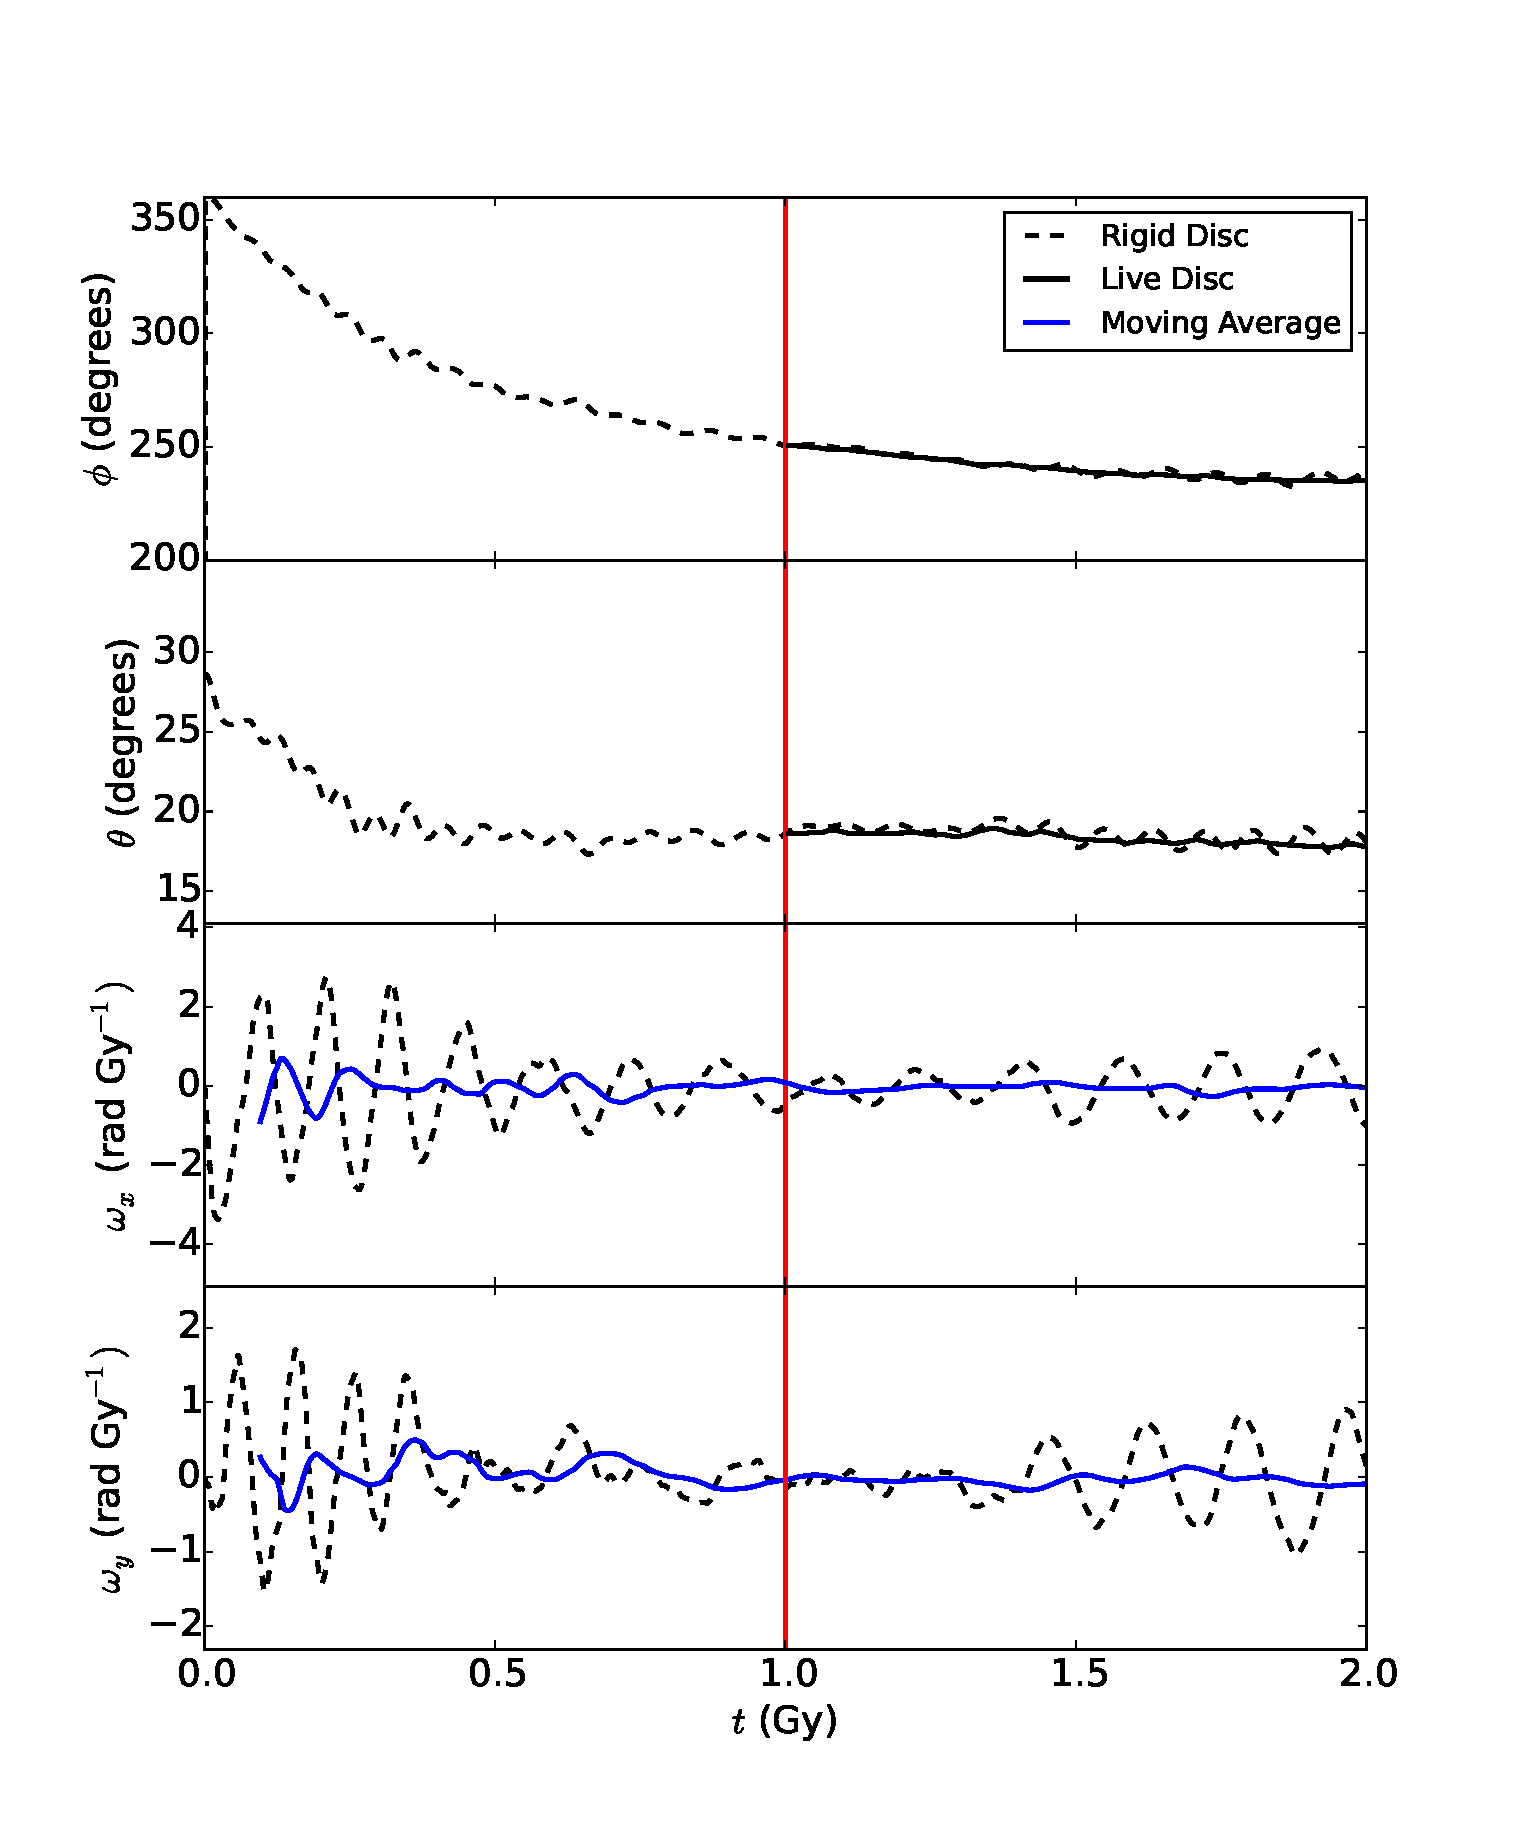
\includegraphics[width=0.9\textwidth]{../figures/flattened_halo_regressions.eps}
\caption{Kinematic variables for the rigid and live discs in an
  isolated, flattened halo as a function of time.  The upper two
  panels show the Euler angles $\theta$ and $\phi$ for the rigid disc
  (dashed curves) and live disc (solid curves) where the live disc is
  introduced at $t=1\,{\rm Gyr}$ (red vertical line).  The bottom two
  panels show the $x$ and $y$ components of the angular velocity, as
  measured in the body coordinate system.  In these two panels the
  solid curves show the $\delta t \sim 150\, \text{My}$ moving
  average, which is used to initialize the live disc.}
\label{fig:flattened_halo_regression}
\end{figure}
  
Fig. \ref{fig:flattened_halo_regression} shows the Euler angles and
angular velocity components for the rigid and live discs as a function
of time.  The time-dependence of $\omega_x$ and $\omega_y$ is
characterized by an interference pattern between short $\sim 125\,{\rm
  Myr}$ period nutations and a decaying long-period
precessional motion. Note that $\theta$ and $\phi$ for the live disc
track the corresponding values for the rigid disc for $t>1\,{\rm
  Gyr}$.  By initializing the live disc with the angular velocity of
the rigid disc, we capture the (small) precessional motion of $\sim
10^\circ {\rm Gyr}^{-1}$ between $t = 1\,{\rm Gyr}$ and $2\,{\rm
  Gyr}$.  The disc settles into a preferred plane within the first
$300\,{\rm Myr}$ that is intermediate between its initial symmetry
plane and the initial symmetry plane of the halo. More precisely, the
vector of the new minor axis is $\textbf{c} = [-0.159,0.146,0.976]$
measured at $20\text{ kpc}$, $12.5^{\circ}$ from the original
flattening axis.

\begin{figure}
\centering 
\includegraphics[width=0.9\textwidth]{../figures/Flattened_Selected_Density_Panels.eps}
\caption{Face-on projections of the particle distribution for two
  snapshots of a live disc in a flattened
  halo. The solid line for scale is 25 kpc with a centre
  coincident with the disc's. }\label{fig:flattened_disk_warps}
\end{figure}

\begin{figure}
\centering
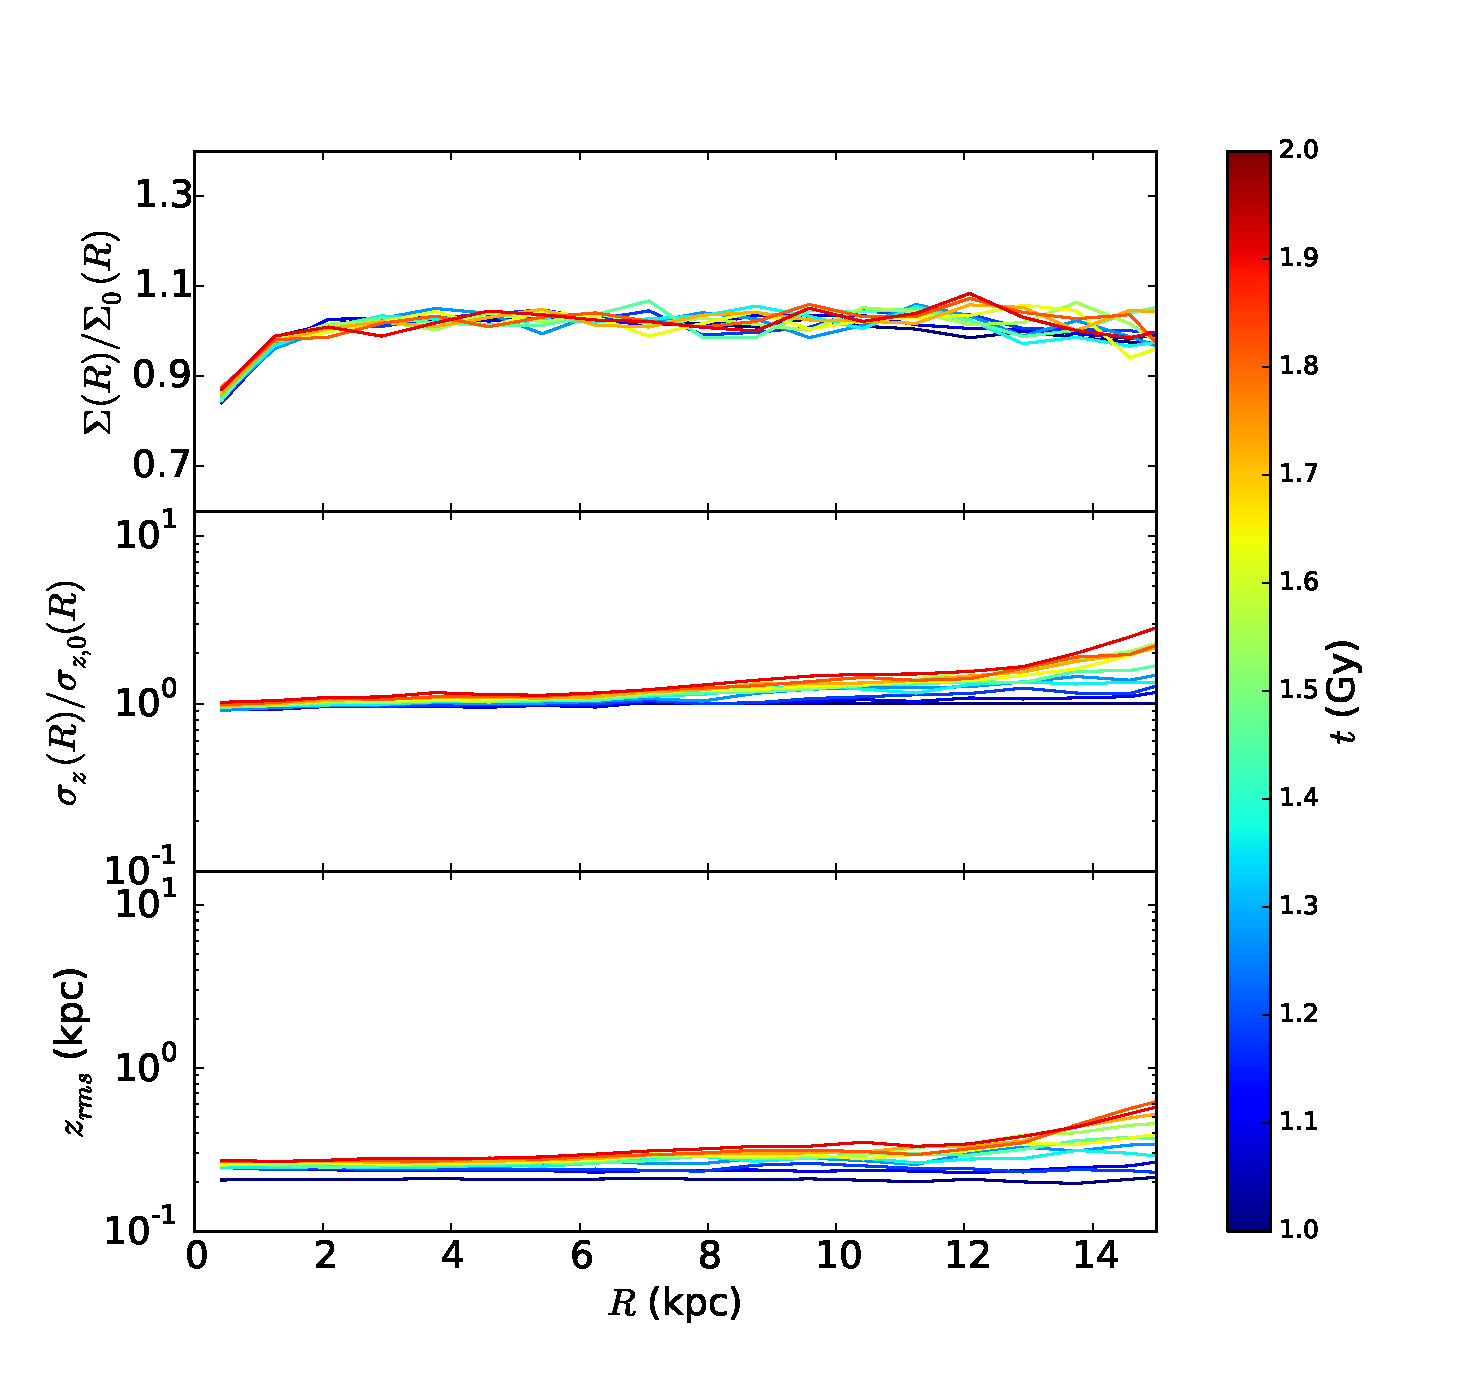
\includegraphics[width=0.9\textwidth]{../figures/flattened_surface_densities_fixed.eps}
\caption{Surface density, vertical velocity dispersion, and scale
  height profiles as a function of Galactocentric radius $R$ for 10
  snapshots equally spaced in time.  The top panel shows the surface
  density $\Sigma(R)$ divided by
  $\Sigma_0(R) = \left (M_d/2\pi R_d^2\right )\exp{\left[-\left
        (R/R_d\right ) \right]}$
  in order to highlight departures from a pure exponential disc.
  Likewise, in the middle panel, we show the ratio
  $\sigma_z(R)/\sigma_{z,0}(R)$ where $\sigma_{z,0} = \exp{(-R/2R_d)}$.
  The bottom panel shows the RMS $z$ as a function of $R$. }
\label{fig:flattened_surface_densities}
\end{figure}

Fig. \ref{fig:flattened_disk_warps} shows surface density maps for the
disc at two snapshots.  The disc develops a weak warp due to its
interaction with the halo.  The development of the warp is also
evident in the surface density, vertical velocity dispersion, and
scale height profiles shown in
Fig. \ref{fig:flattened_surface_densities}.  We see that the surface
density within $\sim 15\,{\rm kpc}$ or $6R_d$ is essentially unchanged
while at larger radii, there are $10-20\%$ time-dependent
fluctuations.  The scale height $\langle z^2\rangle^{1/2}$ increases
with time and radius.  At early times, the increase is most prominent
beyond $\sim 15\,{\rm kpc}$ while at late times, the scale height
increases more smoothly from the center to the edge of the disc.

\section{Cosmological Simulations}

We now use our method to insert a live disc with prescribed structural 
properties into a cosmological halo.  In this section, we focus on 
disc dynamics while in the next, we consider the effect the disc has 
on the dark halo. 

\begin{figure}
\centering
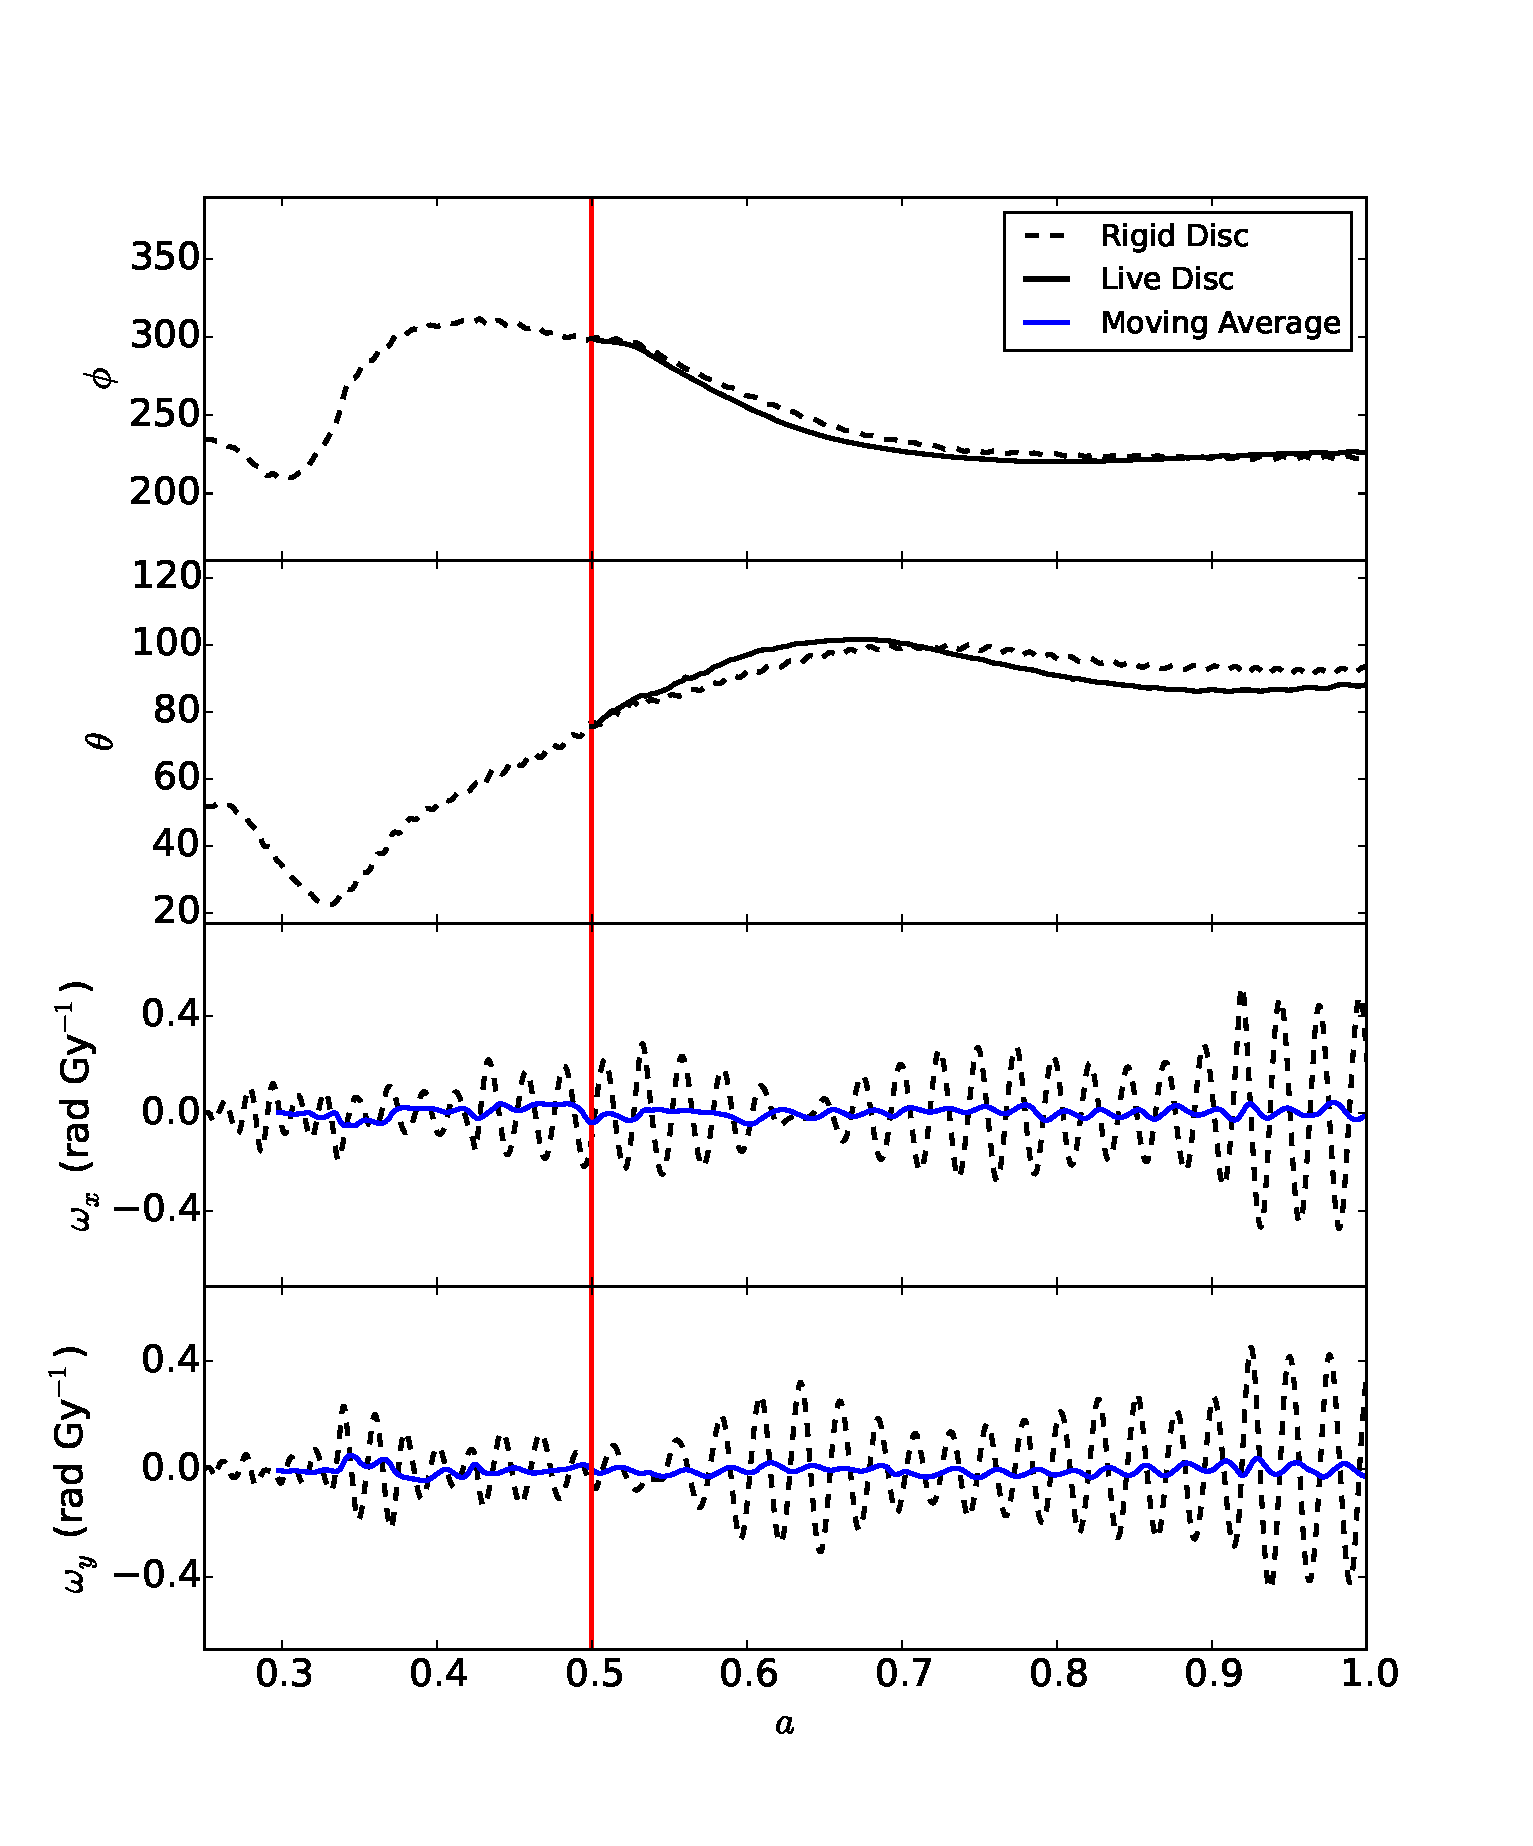
\includegraphics[width=0.9\textwidth]{../figures/cosmo_halo_regressions.eps}
\caption{Kinematic variables for the rigid and live discs in our
  cosmological halo as a function of scale factor $a$.  Line types are
  the same as in Fig. \ref{fig:flattened_halo_regression}.  The live
  disc is introduced at a redshift $z=1$ when the scale factor is
  $a=0.5$ (red vertical line). The blue line shows the $\delta a \sim
  0.04$ moving average calculated by averaging the last 300 points in
  the disc integration routine.} \label{fig:cosmo_inclination}
\end{figure}

In Fig.\,\ref{fig:cosmo_inclination} we show the kinematic variables
for the rigid and live discs in the RD and LD simulations.  The two
simulations are identical prior to $z=1$ ($a=0.5$) when the live disc
is swapped in for the rigid one.  The short period ($300\,{\rm Myr}$)
oscillations in $\omega_1$ and $\omega_2$ are nutations.  To
initialize the live disc, we use the fixed-window moving average of $\omega_x$ and
$\omega_y$.  By and large, the Euler angles of the rigid and live
disc's track one another for $z<1$, indicating that the rigid disc
is a reasonable model for a live one, at least in terms of the disc's
orientation.

\begin{figure}
\centering 
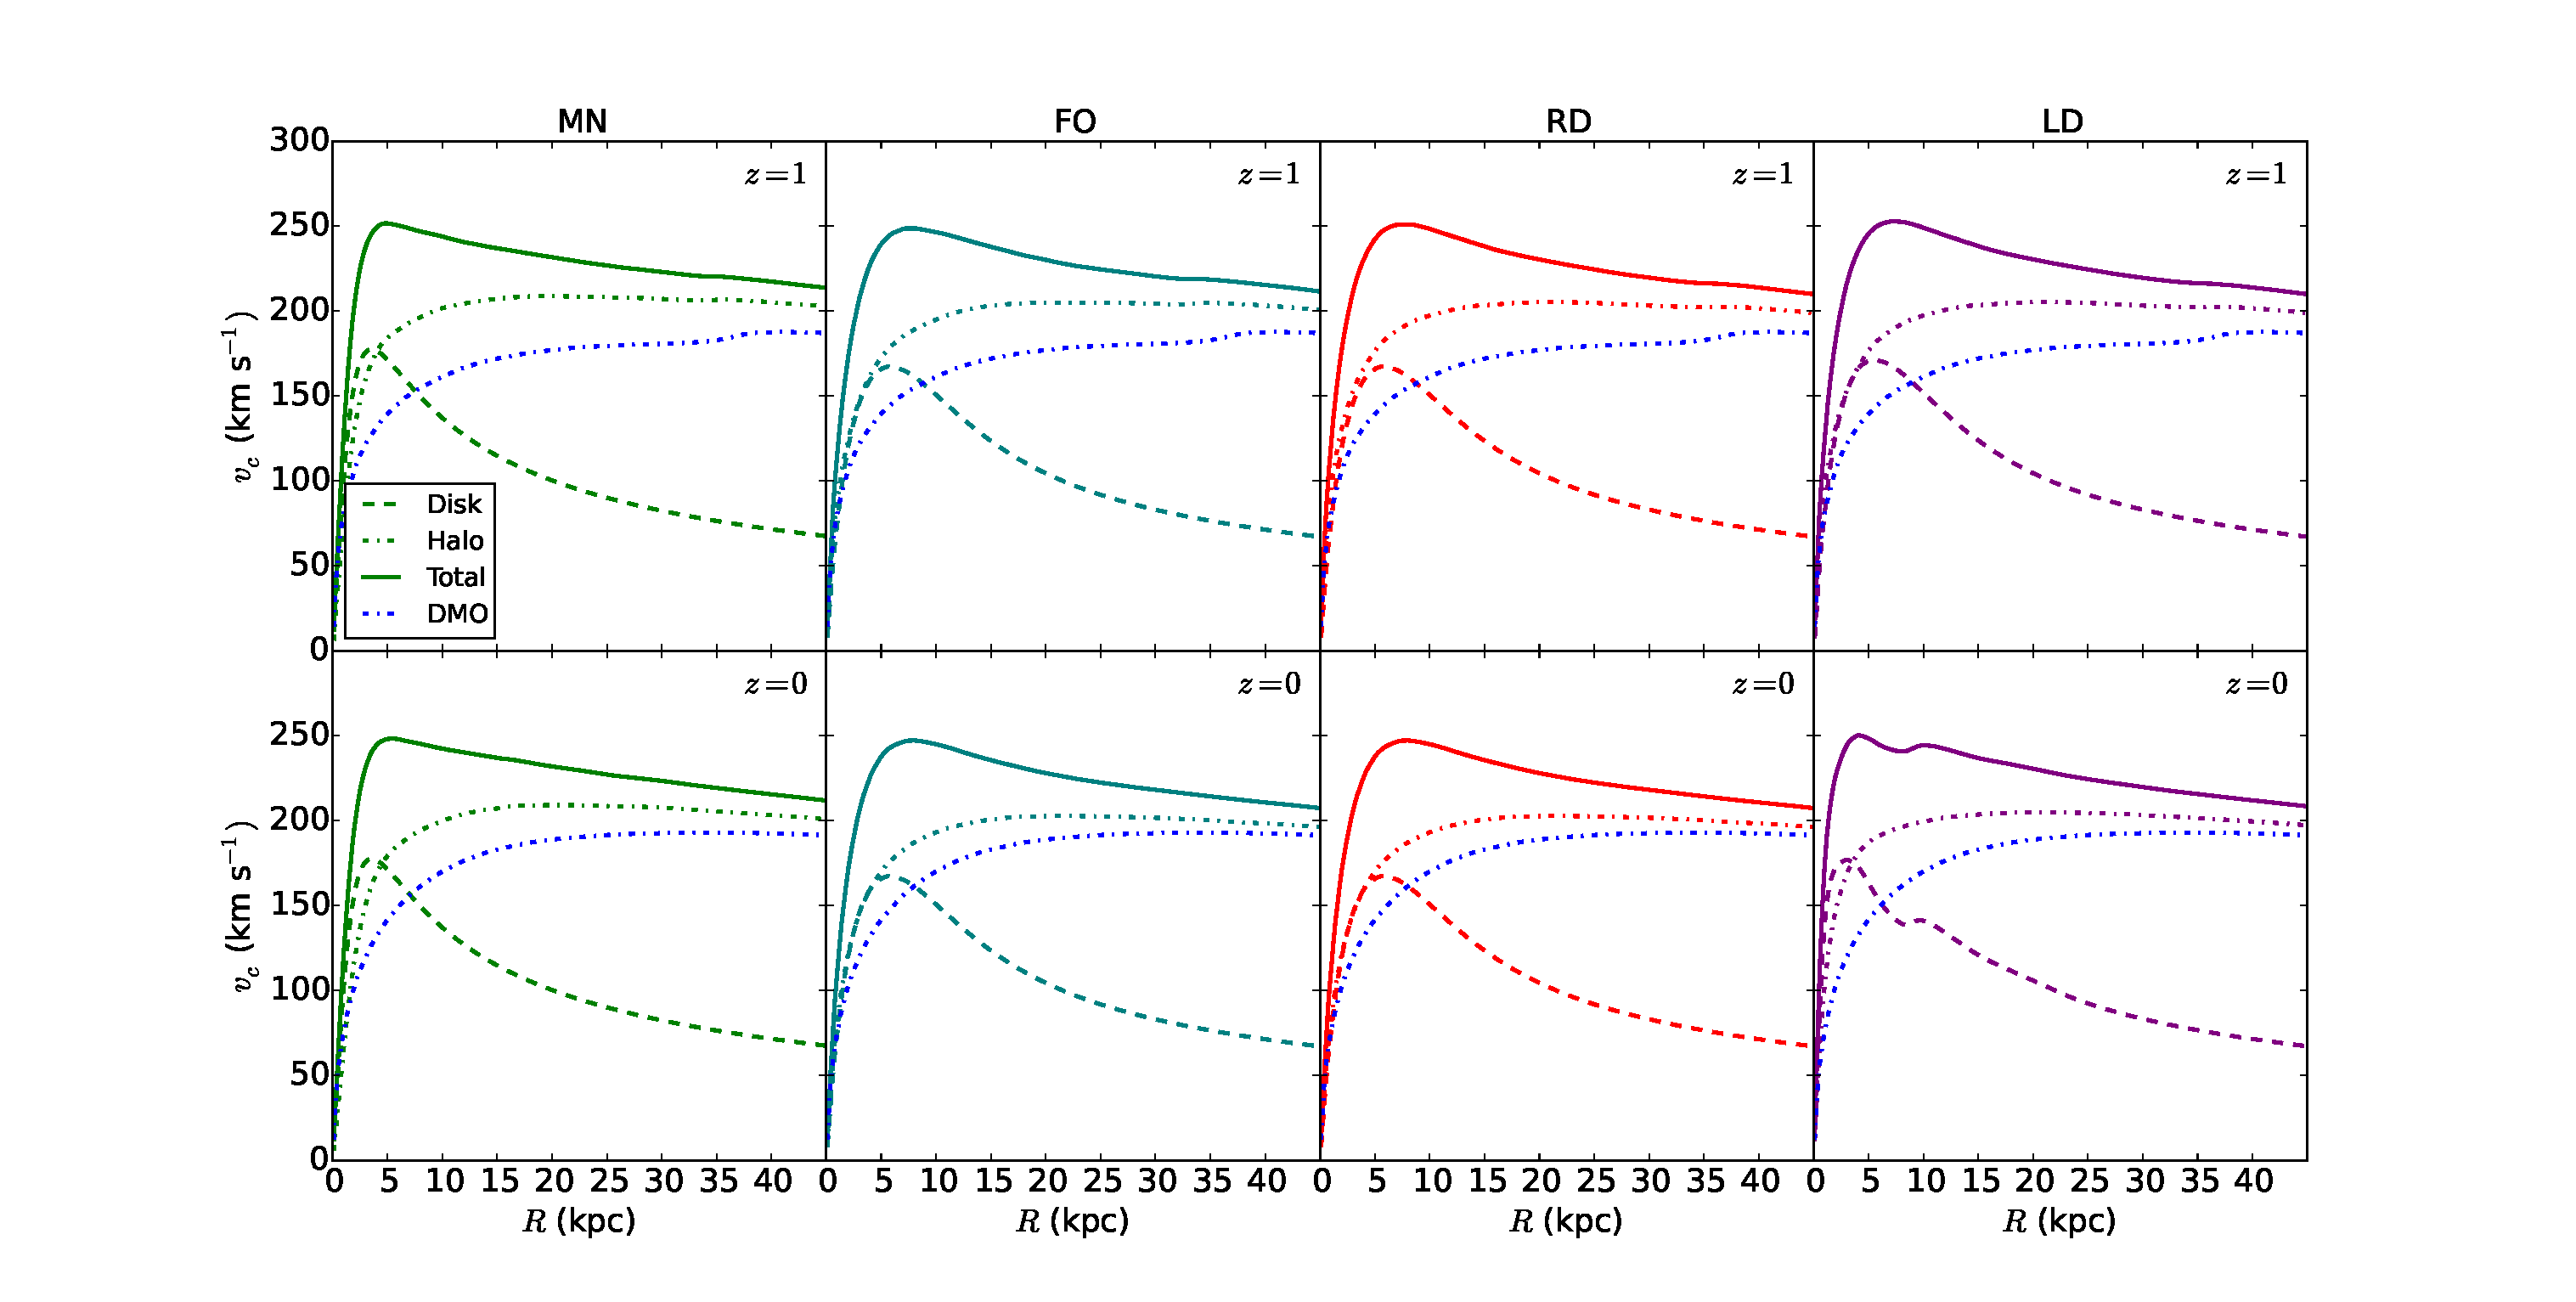
\includegraphics[width=1.\textwidth]{../figures/all_rotation_curves_five_sims}
\caption{Circular speed curve decompositions at $z=1$ (top row) and
  $z=0$ (bottom row) for (from left to right) our MN, FO, RD, and LD
  simulations.  Halo contributions are represented as dot-dashed
  lines, disc contributions are represented by dashed lines, and the
  total rotation curve is given by a solid line.  For reference, we have
  included the circular speed curve for the DMO halo (dot-dashed curve).}
\label{fig:rotation_curves}
\end{figure} 

In Fig.\,\ref{fig:rotation_curves} we show the circular speed curves
at $z=1$ and $z=0$ for our four simulations.  We see that the disc in
our model is submaximal.  To be precise, we have $V_d/V_c \simeq 0.68$
at $R=2.2R_d$ where $V_d$ is the circular speed due to the disc and
$V_c$ is the total circular speed.  In short, the contributions from
the disc and halo to the centrifugal force are approximately equal at
a radius where the disc contribution reaches its peak value.  By
comparison, a maximal disc is generally defined to have $V_d/V_c >
0.85$ \citep{sackett1997}.  If we use $V_d/V_c$ at $2.2R_d$ as the
defining characteristic of the model, then our simulations match up
with the F-5 simulation of
\citet{YurinSpringelStellarDisks}, although our discs are slightly
warmer, with a Toomre Q-parameter of $1.4$ as compared with $Q\simeq
0.9$ for their discs and our discs are thinner ($200\,{\rm pc}$ vs.
$600\,{\rm pc}$). We note that in a two-integral disc DF, $Q$ and the
disc thickness are linked whereas in a three-integral DF, they can be
set independently.  The method of \citet{YurinSpringelGalic} can be extended to consider
a three-integral DF, but these models were not considered in  \citet{YurinSpringelStellarDisks}. Moreover, their two-integral model, 
which imposes $\sigma_R=\sigma_z$, violates the epicycle approximation,
leading to transient system behaviour at early times when disc bars
first form.

%\textbf{Although the GalIC code can be extended to consider models for which $\sigma_R \neq \sigma_z$, these models will not be in equilibrium as GalIC does not enforce consistency with the epicycle approximation \citep{AumerBinneyGalICComments}}.
%In other words, the models considered in
%\citet{YurinSpringelStellarDisks} are a restricted subset of possible
%disc models.

The circular speed curves in Fig. \ref{fig:rotation_curves} show little change exterior to $\sim 2R_d$
after $z_l$, thus providing another indication that the live disc
was close equilibrium when it was swapped in for the rigid one. The
formation of a bar is evident in the circular speed, and we can infer
the bar contributes substantially inside $2.2 R_d \simeq 8$\,kpc.  The halo contribution at $R=2.2R_d$ is about 20\% larger
in the four disc runs than in the DMO one due to adiabatic
contraction.  Interestingly, the halo in the MN run shows
somewhat more contraction than in the RD and LD runs.  We note that in
the MN run, the disc potential tracks the potential minimum of the
halo whereas in the RD/LD case, the disc's position is determined from
Newtonian dynamics.  In general, the centre of the disc tracks the
halo potential minimum so long as the potential changes slowly with
time.  However, during a major merger (and indeed, just such an event
occurs at $z=2$) there are rapid changes in the halo potential and 
the position of the disc, as determined by Newtonian dynamics, can
differ significant from the minimum of the halo potential.  Evidently,
the {\it ad hoc} prescription of growing a disc at the halo's
potential minimum may, in some cases, over-estimate the effect of
adiabatic contraction.

\begin{figure}
\centering
\includegraphics[width=0.9\textwidth]{../figures/Selected_Density_Panels.eps}
\caption{Projected density along three orthogonal directions for the
  live disc at four epochs between $z=1$ and $z=0$.  The projections are presented
  in physical units. The solid line for scale is
  37 kpc with a centre coincident with the disc's.}
\label{fig:cosmo_density_panels}
\end{figure}

\subsection{Bar Formation}

In Fig.\,\ref{fig:cosmo_density_panels} we show orthogonal projections
of the disc density in our LD simulation at four epochs between
$z=1$ (lookback time of 7.9 Gyr) and the present epoch.
During the first billion years of live disc evolution, the disc
develops a bar and spiral structure.  In addition, there is a
warp in the outer disc extending several kiloparsecs above the midplane
of the inner disc.  By the present epoch, the bar has grown in length and
intensified and the edge-on view shows the classic X-pattern.

We consider the usual parameter bar strength $A_2 = 
|c_2|$ where

\begin{equation}
c_m = \frac{1}{M_S}\sum_{j\in S} m_j e^{im\phi_j}~.
\end{equation}

\noindent Here, $S$ is some circularly-symmetric region of the disc
(e.g., a circular annulus) and the sum is over all particles labeled
by $j$ and with mass $m_j$ that are inside $S$.  We find that
$A_2$ for the inner $2R_d$ of the disc reaches $0.43$ at $t=6.7\,{\rm
  Gyr}$, decreases to $0.36$ by $t= 9.2\,{\rm Gyr}$, presumably
because the bar has buckled, and then increases to $0.47$ by the
present epoch.  On the other hand, $A_2$ for the entire disc increases
to $0.27$, decreases to $0.23$, and then increases to $0.28$ for the
same epochs.  Note that the inner $2R_d$ of the disc contains $60\%$
of the mass.  Thus, the fact that $A_{2,2R_d}/A_{2,{\rm tot}}\simeq
  0.6$ implies that most of the bar mass resides within the inner
  $2R_d$.

The bars in \citet{YurinSpringelStellarDisks} seem to be stronger then
then ones in our simulations --- they find $A_2\simeq 0.6$ but use a
non-standard formula for $A_2$.  Moreover, their bars appear to extend
across most of the disc.  In terms of disc dynamics, the main
difference between our simulations is the fact that we use a
three-integral DF for the disc whereas they use a two-integral DF.  In
the latter, the velocity dispersion in the radial and vertical
directions are the same.  Thus, the radial dispersion, which fixes the
Toomre $Q$ parameter, also determines the thickness of the disc.  We
note that their initial discs are a factor of two or three thicker
than ours.  We speculate that the bars that develop in these thick
discs are less susceptible to buckling and therefore able to grow
stronger and longer.  These ideas will be investigated in more detail
in a future publication.

\subsection{Kicked-up Stars and Disc Heating}

The outer part of the disc suffers considerable disruption and warping
presumably through its interaction with the main halo or substructure.  The right-most
panel of the $a=0.55$ snapshot in Fig. \ref{fig:cosmo_density_panels}, for example, shows a classic
integral-sign warp.  The other snapshots show that a significant
number of disc particles have orbits that now take them to high
galactic latitudes.

\begin{figure}\centering 
 \includegraphics[width=0.9\textwidth]{../figures/surface_densities.eps}

  \caption{Surface density, vertical velocity dispersion, and scale
    height profiles of the live disc for 10 snapshots equally spaced
    in scale factor $a$ between $a=0.5$ ($z=1$) and $a=1$ (present
    epoch).  Panels are the same as in
    Fig. \ref{fig:flattened_surface_densities}.}
\label{fig:surface_densities} 
\end{figure}

The impressions one has from the density projections are borne out in
Fig.\,\ref{fig:surface_densities} where we show the surface density
and scale height profiles at different times.  Bar formation
redistributes mass in the disc leaving a deficit (relative to the
initial exponential disk) between $5$ and $15\,{\rm kpc}$.  The disc
becomes thicker and its vertical velocity dispersion increases though
a combination of disc-halo interactions and the effects of the bar and
spiral structure \citep{gauthier2006, dubinski2008, kazantzidis2008}.

A striking feature of the simulations are the streams of disc stars
well above the disc plane.  These stars may represent an example of a
kicked-up disc, which has been seen in other N-body simulations
\citep{PurcellHeatedDisk, McCarthyHeatedDisk} and invoked to explain
kinematic and spectroscopic observations of M31
\citep{DormanKickedUpDisk} and the Monoceros Ring \citep[e.g.][]{monoceros_disc,ibata_et_al_2003}. The idea is that interactions between the
disc and both satellite galaxies and halo substructure liberate stars
from the disc, launching them to regions of the galaxy normally
associated with the stellar halo.  Our live disc simulation
corroborates this hypothesis and is in broad agreement with previous
numerical work. 

Finally, we note that the $a=1$ panel of Fig. \ref{fig:cosmo_density_panels}
shows a relatively thin, stream-like structure, above the disc which
is qualitatively similar to the Anti-centre Stream \citep[ACS,][]{acs_disc}. While the ACS
is believed to be due to the disruption of a globular cluster \citep[e.g.][]{acs_disc}, Fig. \ref{fig:cosmo_density_panels} suggests that perturbations to the disc can create similar features. Intriguingly, \citep{de_boer_et_al_2017} recently 
found that the ACS is rotating in the same sense as the Milky Way disc.


%{\bf There is also some basis for believing that there are similarly 
%kicked up disc stars in the Milky Way.  The Monoceros Ring is a Milky Way 
%structure composed of low-metallicity stars in a narrow range of Galactocentric
%distances (15-20 kpc) \citep{newberg2002, yanny2003, monoceros2005}. Two 
%competing hypotheses for the formation of the Monoceros stream of stars are
%a dwarf galaxy on a near circular orbit at low Galactic latitude, or displaced
%disc stars. Recent simulation and observational work suggests that the latter of
%these hypotheses could be at work in the Milky Way \citep{NewbergRadialWaves, gomezwarps}.
%Because our method allows us to study the evolution of an initially cold population of
%disc stars, we can resolve structures like the Monoceros Ring.  The fact that we find
%a similar structure in the one simulation we ran suggests, with existing work, that 
%perturbations to the disc's vertical structure may be a commonplace mechanism for 
%generating streams of stars coincident with the discs of galaxies.}

\section{Halo Substructure in the Presence of a Disc}

In this section, we consider the effect of a disc on a halo's
structural properties such as its spherically-averaged density
profile, its shape, and its subhalo population.  An examination of the
DMO simulation shows that the halo we have selected builds up through a
series of mergers and accretion events, but that by $z=1$ it has
settled into a relatively relaxed state with an NFW profile that
evolves very little between $z=1$ and $z=0$ within the inner 100 kpc.  Our sequence of
simulations, (MN, FO, RD, and LD) allow us to tease out the effects of
different disc insertion methods.  The MN simulation, for example,
pins the centre of the disc to the minimum of the halo potential,
whereas the other simulations dynamically evolve the position and
velocity of the disc potential via Newtonian mechanics.  The MN and FO
simulations both assume that the orientation of the disc potential
during the growth phase is fixed whereas RD and LD solve for the
orientation using rigid body dynamics.
 
\subsection{Global Properties of the Halo}

\begin{figure} \centering 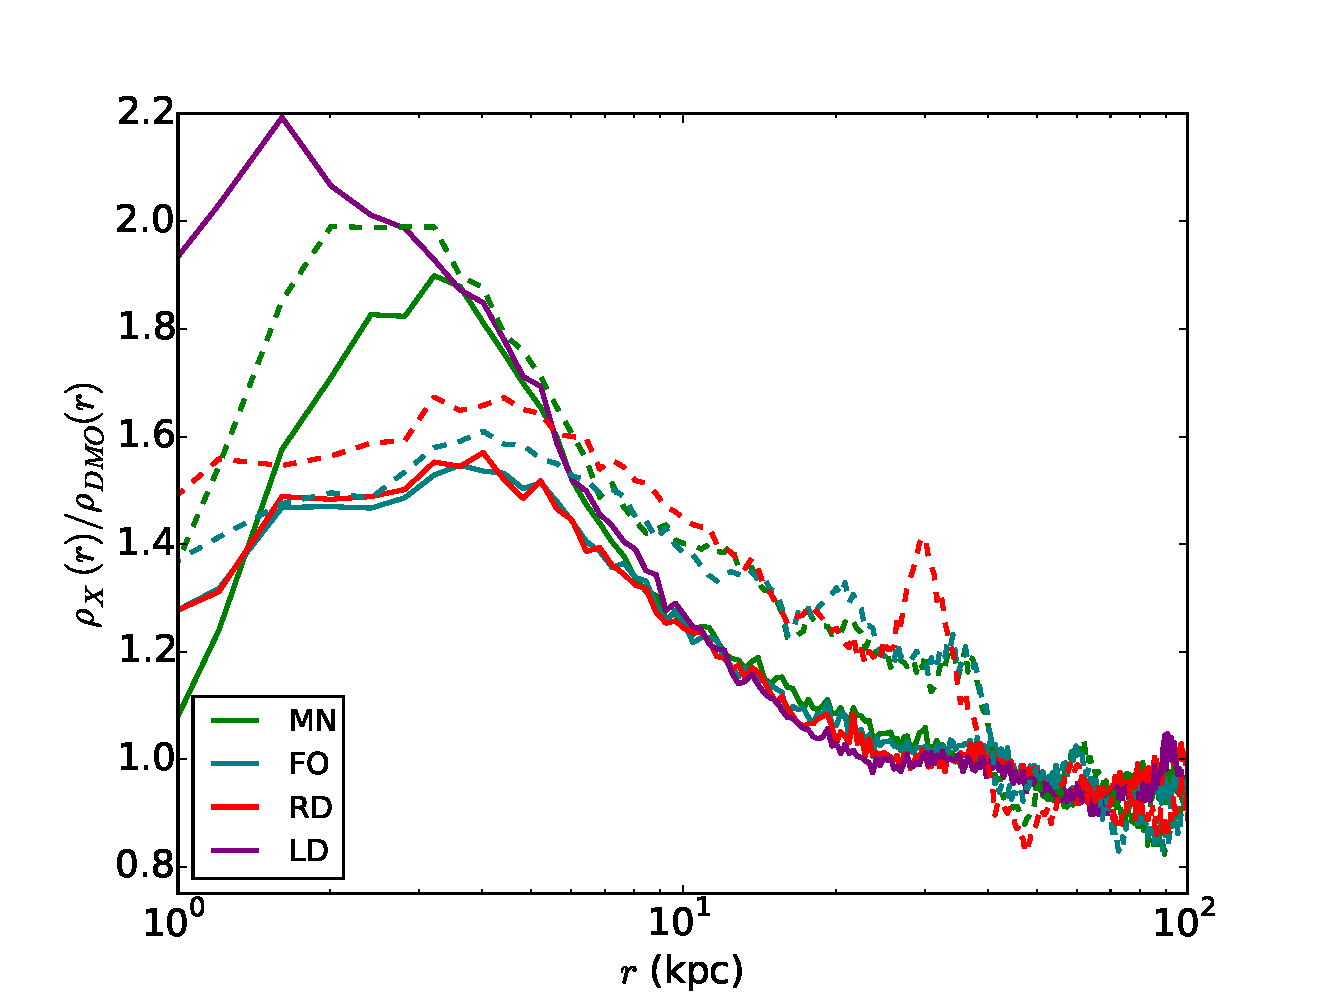
\includegraphics[width=0.9\textwidth]{../figures/halo_density_ratios_five_sims.eps} 
  \caption{The ratio of halo density to the DMO simulation for MN
    (green), FO (teal), RD (red), and LD (purple) at $z=1$ (dashed)
    and $z=0$ (solid). The presence of the disc significantly increases the central concentration of the halo.}
\label{fig:halo_ratios}
\end{figure}

In Fig.\,\ref{fig:halo_ratios} we show the ratio of the
spherically-averaged density profile in the four disc runs to that
from the DMO run.  At $z=1$ the haloes in the FO, RD, and MN runs show
evidence for adiabatic contraction with the density in the inner $\sim
30\,{\rm kpc}$ increasing by a factor of $1.2-2.1$.  The effect is
strongest in the MN simulation, which is to be expected since the halo
in that case always sees the disc potential at the minimum of its
potential.  Of course, this prescription is unphysical.  In general,
and especially during a major merger, the disc and halo potential
minimum will not necessarily coincide.

Between $z=1$ and $z=0$, the mass of the disc is constant.  Adiabatic
contraction ceases but the halo still responds to the time-varying
disc potential.  Interestingly, at intermediate radii (between
$\sim 10-40\,{\rm kpc}$) the density profile of the halo settles back
to a state close to that found in the DMO run.  Perhaps most striking
is the fact that the halo in the LD run becomes more centrally
concentrated than the halo in any of the other cases.  One possible explanation
is that dynamical friction from the disc drags dark matter subhaloes
toward the centre of the halo where they are tidally disrupted.

\begin{figure} 
\centering 
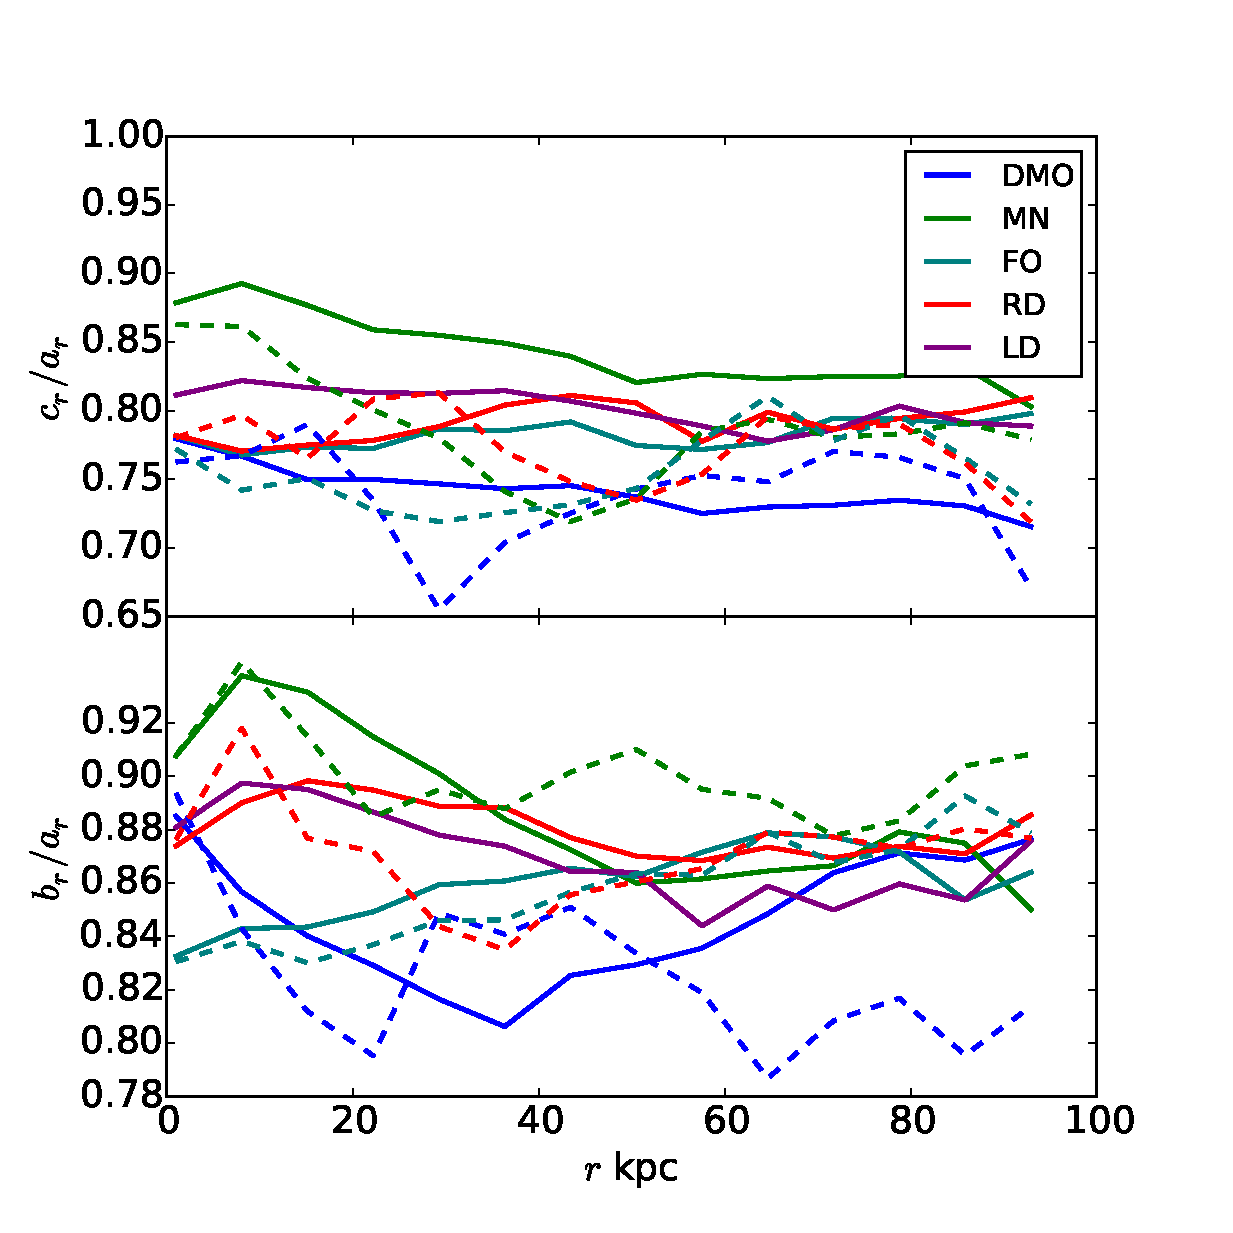
\includegraphics[width=0.9\textwidth]{../figures/eigenratios_vs_radius.eps} 
\caption{Axis ratios as a function of radius.  Shown are the
  minor-to-major axis ratio (top panel) and the intermediate-to-major
  axis ratio (bottom panel) at $z=1$ (dashed curves) and $z=0$ (solid
  curves).  Blue corresponds to DMO, green to MN, teal to FO, red to RD, and
  purple to LD.}
\label{fig:axis_ratios}
\end{figure}

In Fig.\,\ref{fig:axis_ratios} we show the minor-to-major ($c_r/a_r$)
and intermediate-to-major ($b_r/a_r$) axis ratios as a function of
radius for both the $z=1$ and $z=0$ snapshots.  The axis ratios are
calculated by diagonalizing the moment of inertia tensor in
linearly-spaced radial shells.  The DMO halo is triaxial with
$c_r/a_r\simeq 0.75$ and $b_r/a_r\simeq 0.85$.  Note that the axis
ratio profiles are smoother at $z=0$ than at $z=1$, which supports the
observation that the halo has settled into a more relaxed state over
the past $7$ or so billion years.  In general, discs tend to make
halos more spherical, a result that has been known for some time from
both collisionless and hydrodynamical simulations
\citep[e.g.][]{dubinski1994_ApJ431_617,Zemp2012}.


Evidently, the MN halo is rounder, especially in the inner part, than
the FO halo.  Recall that the main difference between these two cases
is that the MN disc is pinned to the potential minimum of the halo.
It is perhaps not surprising then that, as with adiabatic contraction,
it has a stronger effect on the halo's shape.  
We also note that the axis ratio profiles for the RD and LD simulations
are fairly similar.  

\subsection{Subhalo Populations}

We now turn our attention to halo substructure.  We identify subhaloes
and determine their positions and masses using \textsc{rockstar}
\citep{rockstar}, which employs a friends-of-friends algorithm in six
phase space dimensions.  We consider only those subhaloes with mass
$m_s$ between $m_{\rm min} = 10^{7.5}\,M_\odot$ and $m_{\rm max} =
10^{10.5}\,M_\odot$.  Subhaloes at the lower end of this range are
marginally resolved with $\sim100$ particles, above which the subhalo
mass can be trusted \citep[e.g.][]{onions_et_al_2012}, while those at the upper end contain $\sim 3\%$ of
the halo's virial mass.

\begin{figure} 
\centering 
{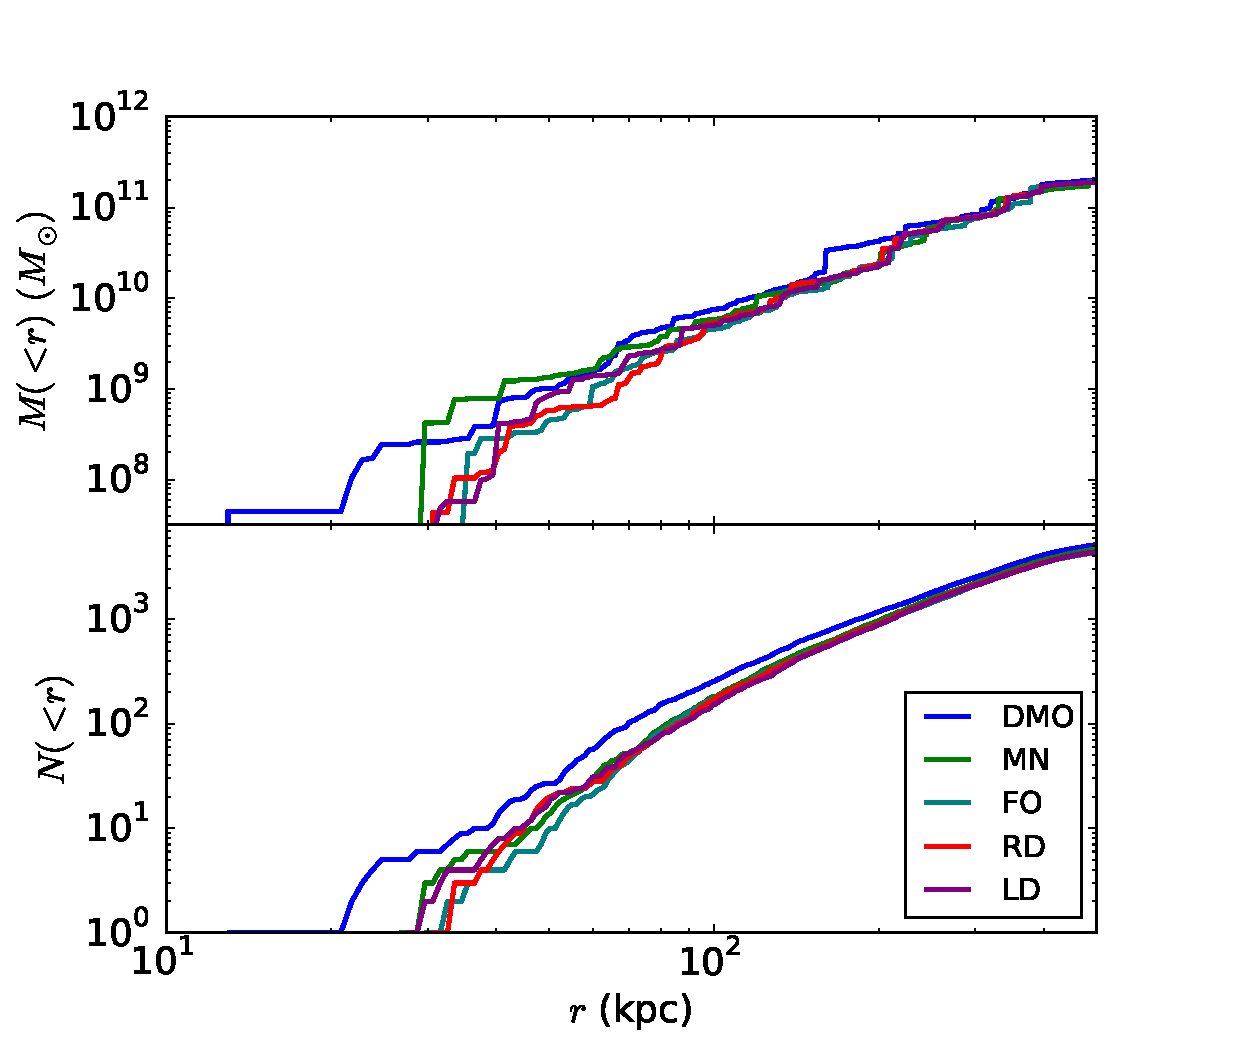
\includegraphics[width=0.9\textwidth]{../figures/cumulative_radial_distribution_five_sims.eps}}
\caption{Cumulative mass in subhaloes inside a radius $r$ (upper panel)
  and cumulative number of subhaloes (lower panel).  We consider only
  subhaloes within $500\,{\rm kpc}$ of the halo centre and with a mass
  above $10^{7.5} M_\odot$.  The curves are blue (DMO), green (MN),
  teal (FO), red (RD), and purple (LD).}
\label{fig:cumulative_distributions}
\end{figure}

\begin{figure} 
\centering 
{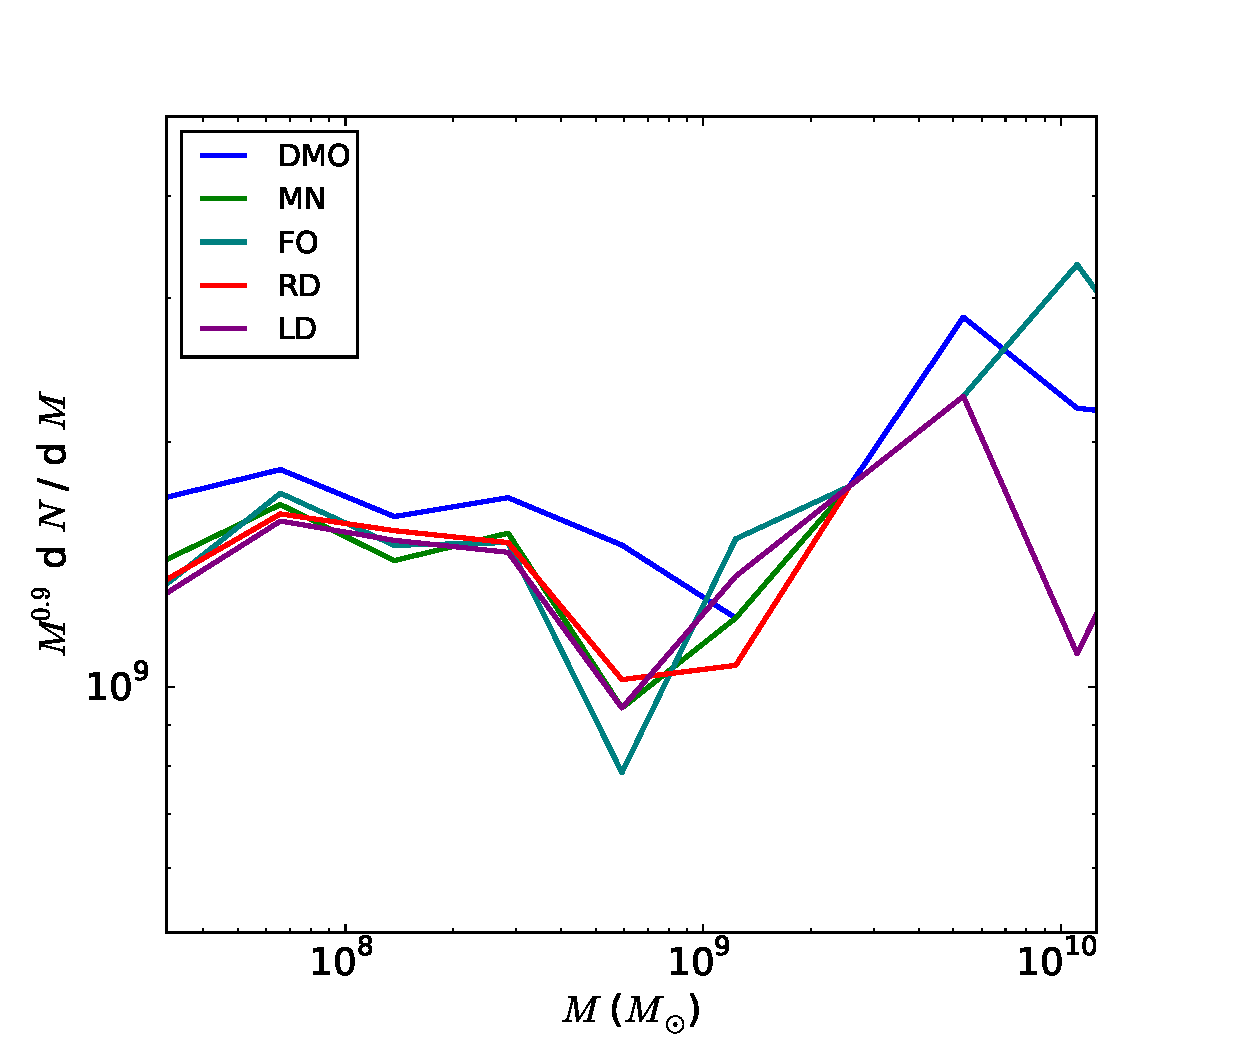
\includegraphics[width=0.9\textwidth]{../figures/differential_halo_mass_fn_five_sims.eps}}
\caption{ Differential mass distribution
  multiplied by $M^{0.9}$ for subhaloes above $10^{7.5} M_\odot$. We
  make an outer radius cut at 500 kpc. The curves are blue
  (DMO), green (MN), teal (FO), red (RD), and purple (LD). }
\label{fig:differential_mass_distributions}
\end{figure}

In Fig.\,\ref{fig:cumulative_distributions} we show the cumulative
mass in subhaloes as a function of Galactocentric radius:

\begin{equation}
M_s\left (<r\right )  = \int_0^r dr \int_{m_{\rm min}}^{m_{\rm
    max}} dm_s\,m_s\,\frac{d^2 N}{dm_s\,dr}
\end{equation}

\noindent We also show the cumulative number of subhaloes.  In
general, the presence of a disc depletes substructure inside about
$30\,{\rm kpc}$ but leaves the outer substructures unaffected.

We next consider the differential mass distribution as a function of
subhalo mass.  Recall that for a pure dark matter halo,
$dN/d\ln(m_s)\propto m_s^{-p}$ where $p\simeq 0.9$
\citep[e.g.][]{gao2004}.  In
Fig. \ref{fig:differential_mass_distributions}, we therefore show the
quantity $m^{0.9}\,dN/d\ln(m_s)$ in order to enhance the differences
between the different disc runs.  We see that the halo population
between $m_s \simeq m_{\rm min}$ and $m_s\simeq 10^9\,M_\odot$ is
depleted, but only by about $20-30\,\%$.  Taken together,
Fig.\,\ref{fig:cumulative_distributions} and
Fig. \ref{fig:differential_mass_distributions} imply that the main
depletion of the subhaloes occurs within the inner regions of the
parent halo, in agreement with \citet{DOhngiaSubstructureDepletion,Sawala2017,GKSubhaloDepletion17}.  That said, the depletion of subhaloes seems rather
insensitive to the disc insertion method, although we caution that only a single halo was used. Our results, being mainly in agreement with previous work, should still be viewed with caution due the consideration of a single host halo.

\subsection{Case Study: A Sagittarius-like Dwarf}

\begin{figure} \centering
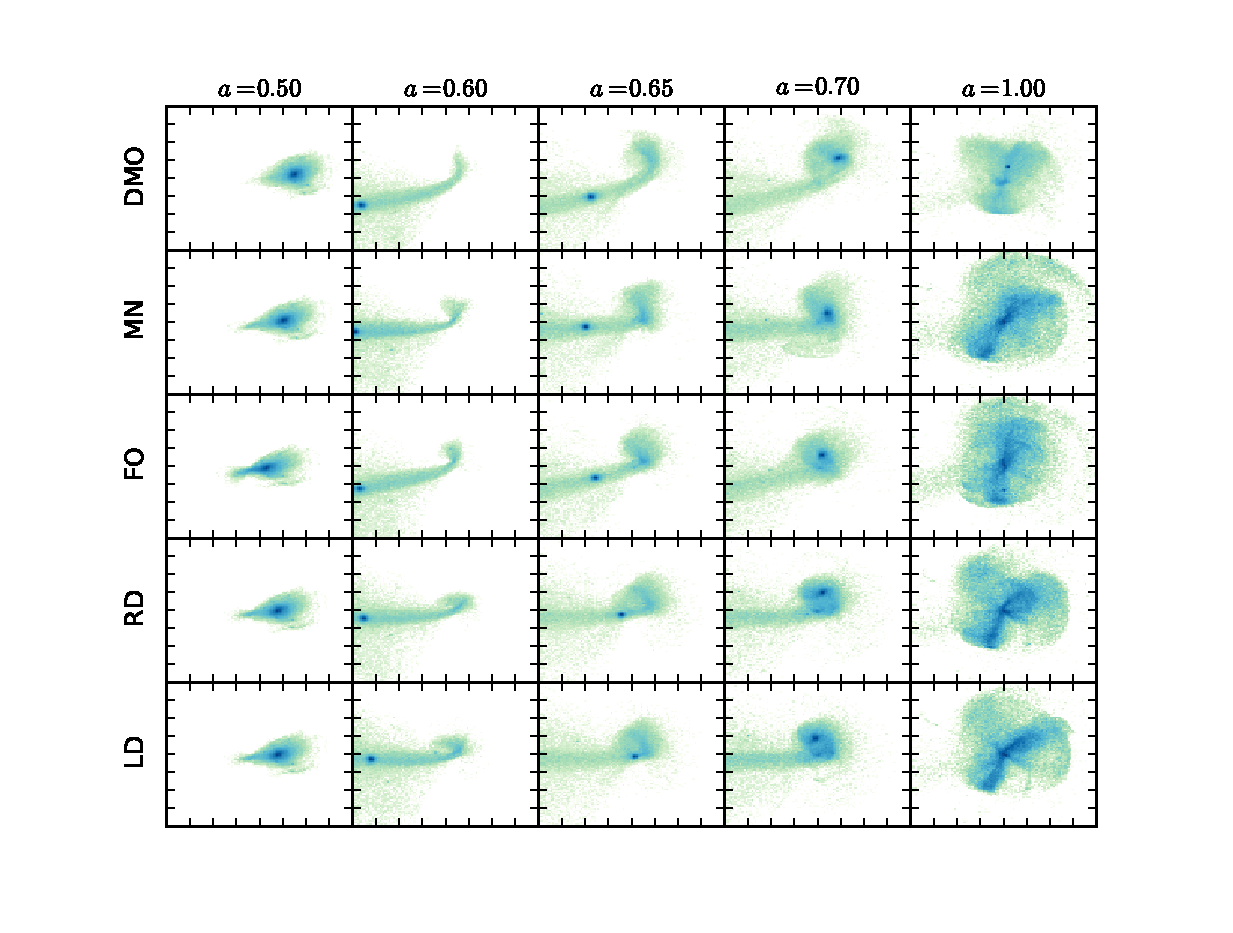
\includegraphics[width=\textwidth]{../figures/streams_side_by_side_five_sims}
\caption{X-Y projections for a selected Sagittarius-like dwarf galaxy. The
  rows from top to bottom are no disc, a fixed Miyamoto-Nagai disc, a
  rigid disc, and a live disc. The scale factors in columns from left
  to right are 0.5, 0.55, 0.6, 0.65, and 0.7. The frame edges are
  $295\,{\rm kpc}$ on each side.}\label{fig:streams}
\end{figure}

Observations of the Milky Way's dwarf galaxies and associated tidal
streams provide a potentially powerful probe of the Galactic potential
and thus the Galaxy's dark halo.  One of the best-studied examples is
the Sagittarius dwarf \citet{ibatadiscovery}.  Fortunately, our
simulation has a satellite galaxy with similar properties, namely, a
dark matter mass of $1.8 \times 10^{10} \, M_\odot$ at
$z=1.0$ and an orbit that takes it close to the disc.  We identify
this object in the five simulations using the \textsc{rockstar}
halo catalogues.  We then gather a list of IDs for all the
bound particles at an early time before the dwarf is disrupted and
follow these same particles in later snapshots using a binary
search tree look-up scheme.  In Fig.\,\ref{fig:streams} we show the
evolution of this subhalo between redshift $z_l=1$ and $z=0$. The
first row shows the baseline evolution in our
DMO simulation.  The dwarf develops leading and trailing tidal tails
during the first few billion years.  By the present epoch, the tidal
debris has dispersed throughout the halo.

The next four rows show the same satellite in our disc simulations.
Perhaps the most noticeable result is that there are stronger features
in the tidal debris at the present epoch once a disc is included.  The
detailed morphology of the tidal debris is certainly different from
one disc simulation to the next.  By eye, debris in MN and FO look
somewhat similar as does the debris in RD and LD. Perhaps the most
noticeable result is that the tidal debris extends to larger galactocentric
radii when a disc is included. The detailed morphology of the tidal debris
clearly depends on the disc insertion method. By eye, tidal debris appears
more isotropic in MN and FO than in RD and LD. The implication is that fixed
potentials are more efficient at disrupting massive satellites than a 
potential which can respond to the satellite's presence.  However, we have
only a single example of massive satellite disruption, and we caution that 
more examples of this behaviour are needed to test this hypothesis.

%\textbf{
%We emphasize that we have only
%looked at one satellite, and that it is unwise to assume that there will
%always be noticeable differences in the disruption patterns.  However, it is
%worth noting that the plausibility of non-equilibrium effects is still a relevant
%conclusion for the direction of debris studies.}

\section{Conclusions}

Simulations in which a stellar disc is inserted ``by hand" into a
cosmological N-body halo provide a compromise between simulations of
isolated disc-halo systems and cosmological simulations that include
gasdynamics and star formation.  Our method builds on the scheme
used by \citet{BerentzenShlosmanStellarDisks,DeBuhrStellarDisks} and refined by \citet{YurinSpringelStellarDisks}.  The basic idea is to introduce, at a redshift $z_g$,
a rigid disc with zero mass into a halo within a cosmological zoom-in
simulation.  Between $z_g$ and $z_l$ the disc is treated as an external
potential with a mass and size that increase adiabatically to their
present day values.  At $z_l$, the rigid disc is replaced by an N-body
one and the simulation proceeds to the present epoch with live disc
and halo particles.


Our method improves upon previous ones in two important ways.  First,
during the growth phase ($z_g > z > z_l$) the position and orientation
of the disc evolve according to the standard equations of rigid-body
dynamics.  Thus, the disc in our scheme receives its linear and angular
momentum with the halo in a self-consistent fashion and is therefore
able to move, precess, and nutate due to torques from the halo.  While
previous methods introduced aspects of rigid-body dynamics during the
growth phase none appear to have implemented the full dynamical
equations have done here \citep{DOhngiaSubstructureDepletion, DeBuhrStellarDisks, YurinSpringelStellarDisks}.

Our sequence MN, FO, RD, and LD of simulations highlights where the
details of the disc insertion scheme are important and where they are
not.  For example, schemes in which the disc tracks the minimum of the
halo potential tend to overestimate the effects of adiabatic
contraction.  On the other hand, the effect of the depletion of halo
substructure seems to be rather insensitive to the details of how the
disc is introduced into the simulation.


Disc insertion schemes such as the one introduced in this paper,
provide an attractive arena for
studies of galactic dynamics. In particular, they allow one to study the interaction between a stellar disc and a realistic dark halo with computationally inexpensive simulations while maintaining some level of control over the structural parameters of the disc.  We fully intend to leverage these advantages in future work.


\section*{Appendix A: Euler's Equations in Comoving Coordinates} \label{sec:derivation}

The time-evolution of the angular momentum vector ${\bf L}$ of a rigid
body acted upon by a torque $\boldsymbol{\tau}$ is given by

\begin{equation}
  \left(\frac{{d} \bf{L}}{{d} t}\right)_f = \left(\frac{{d} \bf{L}}{{d} t}\right)_b  + \boldsymbol \omega \times \bf{L}
  = \boldsymbol{\tau}
\end{equation}

\noindent where the subscripts $f$ and $b$ denote the frame of the
simulation box and the body frame, respectively.  In physical
coordinates, ${\bf L} = {\bf r \times p}$.  Alternatively, we can
write ${\bf L} = {\bf s\times q}$ where ${\bf s} = a^{-1}{\bf r}$
refer to comoving coordinates and ${\bf q} = a^2\dot{\bf s}$ is the
conjugate momentum to ${\bf s}$ (see \citet{QuinnIntegrators}).

For a rigid body, the components of the angular momentum are given by $L_i = I_{ij} \omega_j$ where $i,j$ run over $x,\,y,\,z$ and there is an implied sum over $j$.  Since \textsc{gadget-3} uses comoving coordinates, we write $I_{ij} = a^2 J_{ij}$ where $J$ is the moment of inertia tensor written in terms of the comoving coordinates, ${\bf s}$, rather than the physical coordinates, ${\bf r}$.  For convenience, we define a ``comoving'' angular velocity $\boldsymbol{\varpi} = a^{-2}\boldsymbol{\omega}$.  We then have $L_i = J_{ij} \varpi_j$.  Note that because of the symmetry of our disc, the moment of inertia tensor is diagonal with $J_{xx} = J_{yy}= J_{zz} \equiv J/2$.  The equations of motion for the Euler angles and the disc angular velocity are then given by the standard Euler equations of rigid body dynamics, modified to account for the time-dependence of the disc's moment of inertia:

\begin{equation}
\frac{d\phi}{dt} = a^{-2}\sin^{-1}{\theta} \left (\varpi_x\sin(\psi) + \varpi_y \cos(\psi)\right )~,
\end{equation}
\begin{equation}
\frac{d\theta}{dt} = a^{-2}\left (  \varpi_1\cos(\psi) - \varpi_y \sin(\psi)\right )~,
\end{equation}
\begin{equation}
J\frac{\varpi_x}{dt} + \varpi_x\frac{dJ}{dt}
+ J\varpi_y\varpi_z
=  \tau_x~,
\end{equation}
and
\begin{equation}
\frac{\varpi_y}{dt} + \varpi_y\frac{dJ}{dt}
- J\varpi_x\varpi_z
=  \tau_y~.
\end{equation}

\noindent We have omitted the equations for $\psi$ (rotations in the body frame about the symmetry axis) and $\varpi_z$ since these are determined directly from Eq.\,\ref{eq:omega3}.   
%\def \last_written_page{\thepage}
\bibliographystyle{apalike}
\bibliography{bibliography_paper_i.bib}
%\last_page_of_biblio
%\def \last_written_page{\thepage}

%\chapterbib
%

\chapter{Implementing Disc Insertion Schemes in \textsc{Gadget-3}}\label{ch:implementation}

This chapter is meant to provide more details on exactly how to implement the method described in Chapter~\ref{ch:paper_i}. Example code is included where relevant, but the author believes it is a useful exercise for a new graduate student to implement this themselves, as it tests their understanding of the material in Chapter~\ref{ch:background}. For the purposes of this guide, we are going to assume that the reader has the copy of \textsc{Gadget-3} used for this thesis and has a working understanding of how to use a compiler, MPI, and \textsc{GalactICS}.

\section{Representing a Rigid Disk}

A good deal of time was spent in the early development of the disc insertion scheme thinking about the best way to represent the rigid disc during the growth phase. There were two main approaches we considered. 

The first was to not represent the disc as a physical object in the simulation, but simply as a smooth potential.  In order to compute forces on such an object, one has to rely on Newton's third law. The force (torque) on the disc is equal and opposite to the force (torque) it exerts on every other particle in the simulation. The primary issue with this is that in a tree code or particle mesh code, Newton's third law is violated \citep{barnes_hut, hernquist_1991, GadgetCodePaper}. Furthermore, there is straightforward way to impose periodicity. Since this object exists outside of the tree or particle mesh calculations, it is not accounted for when \textsc{Gadget-3} imposes periodic boundaries.

The second approach, and the one that we used, was to represent the disc as a series of massive particles. We wanted to avoid this initially, since this opens up a wide range of potential problems. The first of these is that you need to explicitly turn off the drift and kick operations for the rigid particles. The segments of code portrayed in Appendix~\ref{ch:predict.c} from \texttt{predict.c} and Appendix~\ref{ch:kicks.c} from \texttt{kicks.c} handle the drift and kick shutoff for collisionless particles respectively. 

In order to initially position the disc, you have to set the initial \texttt{DISK\_X0}, \texttt{DISK\_Y0}, \texttt{DISK\_Z0} variables. The velocity is set by \texttt{DISK\_VX0}, \texttt{DISK\_VY0}, and \texttt{DISK\_VZ0} in units of physical velocity divided by the scale factor (internal simulation units). The initial Euler angles are given as \texttt{DISK\_PHI0}, \texttt{DISK\_THETA0}, and \texttt{DISK\_PSI0}. 

\subsection{Rigid Disk Initial Conditions}

To generate the initial conditions, you need to have the zoom-in snapshot with the halo you want to extract. To set up the rigid disc, we have been using the last snapshot of the zoom-in to create the disc. Using the \textsc{rockstar} positions (converted to kpc) and velocities, run the code provided in Appendix~\ref{ch:extract_halo_ascii.py}. Name the output file to be the path listed in the first line of \texttt{extpot.params}. \textbf{Make sure that the orientation for the rigid disk on the last line of this file is set to be toward the z-axis, or you will rotate the disk twice causing all sorts of bad things!}

Once the disk is finished generating, you need to merge it with the zoom-in particles. Place the unrotated disk at the origin, and the code will place the rigid disk upon initialization. You may use the C++ script I have provided in Appendix~\ref{ch:merge_ics.cpp}. This file will reassign all of the particle IDs and types, so make sure if you use this script that you do not need to preserve the old ones. Make sure \texttt{\#define append} and \texttt{\#define GADGET\_COSMOLOGY} are uncommented.

The disk position, velocity, angular position, and rate of Euler angle change are recorded in \texttt{disk\_vars.txt}. The differences in these quantities from the last timstep are recorded in \texttt{disk\_dvars.txt}. A variety of other quantities are written out into other log files that are pretty self explanatory. Appply \texttt{grep} to the code if you are unsure what a particular log file is. There should be comments.

%\textsc{Gadget-3} should now be run as described. You may occasionally run into an issue where \textsc{Gadget-3} cannot construct a tree and it keeps trying to increase the tree allocation factor.


\section{Integrating the Rigid Body Equations}




\subsection{Initial Parameters and Timestep Selection}
To integrate the disc, you need to set \texttt{RIGID\_PARTICLE\_DISK}, \texttt{ANALYTIC\_LZ}, and a value for \texttt{TULLY\_FISHER\_A}. You will also need a timestep reduction factor, \\\texttt{TIMESTEP\_REDUCTION\_FACTOR}, which reduces the timestep size for the rigid disc integration. We have found that accurately capturing the nutation behavior for the disk generally requires a lower timestep than what \textsc{Gadget-3} assigns from the acceleration.

On the topic of timesteps, you will need to force all of the disk particles into the same timestep bin. Recall how the time integration scheme was described; there is nothing preventing particles in the force tree that are all rigid disk particles from being assigned different timesteps. This is handled by the segment of code from \texttt{timestep.c} in Appendix~\ref{ch:timestep.c}.


\subsection{Integration}

The actual integration scheme is handled in \texttt{rigiddisk.c}. The functions are self-explanatory and implement routines for generating the Euler rotataion matrix. At runtime, the particles in the rigid disk have their relevant quantities (acceleration, torque, etc.) rotated into the frame where the disk axis is the $z$-axis. We solve the angular part of the disk dynamics in this frame using the implicit Euler method. For the actual timestep used in the integration method, make sure you use the time calculated in \texttt{update\_halo\_positions.c}. This is the actual time elapsed as formulated\footnote{You can check that you're using the right timestep by ensuring the total time elapsed corresponds to the time elapsed in that cosmology.}, not the drift or kick steps given for the conjugate positions and velocities. We apologize for the horrible mess that this section of code has become. Perhaps it would be instructive to write your own halo tracker.

\section{Live Disk Setup and Initial Conditions}

\subsection{Code Setup}
\subsection{Creating Live Initial Conditions}

\section{Known Issues and Pet Peeves}

\subsection{Choosing a Timestep}
\subsection{Integration Scheme}

\bibliographystyle{apalike}
\bibliography{bibliography_implementation.bib}
\chapter{Cosmological Bar Formation: Nature vs Nurture} \label{ch:paper_ii}

\textbf{This chapter contains a reproduction of a paper published in  Monthly Notices of the
Royal Astronomical Society as: Jacob S. Bauer and Lawrence M. Widrow. Can stellar discs in a cosmological setting avoid forming strong bars?. \textit{Monthly Notices of the Royal Astronomical Society}, 476:523-537,
2019. }

\newpage% Abstract of the paper
\section{Abstract}

We investigate the connection between the vertical structure of
stellar discs and the formation of bars using high-resolution
simulations of galaxies in isolation and in the cosmological context.
In particular, we simulate a suite of isolated galaxy models that have
the same Toomre $Q$ parameter and swing amplification parameter but
that differ in the vertical scale height and velocity dispersion.  We
find that the onset of bar formation occurs more slowly in models with
thicker discs.  Moreover, thicker discs and discs in
simulations with larger force softening are found to be more
resilient to buckling, which acts to regulate the length and strength
of bars.  We  simulate disc-halo systems in the cosmological
environment using a disc-insertion technique developed in a previous
paper.  In this case, bar formation is driven by the stochastic
effects of a triaxial halo and subhalo-disc interactions and the
initial growth of bars appears to be relatively insensitive to the
thickness of the disc.  On the other hand, thin discs in cosmological
haloes do appear to be more susceptible to buckling than thick ones and
therefore bar strength correlates with disc thickness as in the
isolated case.  Thus, one can form discs in cosmological
simulations with relatively weak bars or no bars at all provided the
discs as thin as the discs we observe and the softening length is
smaller than the disc scale height.



\section{Introduction}

The problem of bar formation in disc galaxies tests our understanding
of cosmological structure formation and galactic dynamics.  In
principle, theories of galaxy formation should yield predictions for
the fractional distribution of bars in terms of their strength,
length, and pattern speed.  While it is often difficult to make
precise, quantitative statements about bars from observations, general
properties of their distribution have emerged (See
\citet{sellwood1993}, \citet{Sellwood2013} and \citet{BT} for
reviews).  Roughly 25-30 per cent of disc galaxies exhibit strong
bars {(that is bars that dominate the disc luminosity) and another 20 per
cent or more have relatively weak bars \citep{bar_fraction_2,bar_fraction_1, masters2010, Sellwood2013}. } The bar fraction appears to
increase with time.  Approximately one tenth of disc galaxies between
$0.5 \le z \le 2$ have visually identifiable strong bars, which is a
factor of 3-4 smaller than the fraction in the local Universe (see
\citet{simmons2014} and references therein). 

The bar fraction also
varies with galaxy type.  \citet{masters2010} find that $70\pm 5$ per
cent of the so-called passive red spirals have bars as compared to a
$25\pm 5$ per cent bar fraction for blue spirals.  Since the red
spirals are interpreted as old galaxies that have used up their
star-forming gas, this result is consistent with a bar fraction that
increases with time. 

{Further evidence of a colour correlation with galaxy bar fractions was presented in \citet{masters2011}. They also found an increased bar
fraction in galaxies with dominant bulges. Other correlations were explored by \citet{na2010}, who found correlations between bar fractions galaxies of different morphological types and characteristic masses. They also found that central mass concentrations were correlated with different strong bar fractions depending on the morphological type and mass of the galaxies considered. In the same line of thought, \citet{masters2012} found a correlation between the gas content of a galaxy and the likelihood of a strong bar being present.}

{Putting all of these observations together}, 
disc galaxies in the local Universe divide into three
roughly equal bins: those with strong bars, those with weak bars, and
those with no detectable bar.  {These observations suggest that
bars are capable of forming at a wide range of cosmic times, but 
once formed are difficult to destroy. Though bars can, in theory, be
destroyed through an increased central mass concentration, the requisite
mass exceeds typical masses for supermassive black holes \citep{athanassoula_2005}.
}

%\textbf{These observations suggest that bars are 
%capable of forming at a wide range of cosmic times, but once formed,
%are difficult to destroy. Bars can, in theory, be destroyed or weakened 
%by growing a large central mass, but this mass often exceeds typical masses for
%central supermassive black holes \citep{athanassoula_2005}.}

Intuition tells us that properties of a bar should depend on the
properties of its host galaxy and the environment in which that
galaxy lives.  Theoretical arguments indicate that cold, thin discs
are susceptible to local ``Toomre'' instabilities {\citep{BT}}.  
Furthermore, discs that are strongly self-gravitating, that is discs that 
contribute the bulk of the gravitational force required to maintain their rotational
motion, are susceptible to global instabilities.  Thus, one can
construct initially axisymmetric galaxy models that form bars with
vastly different properties (or no bars at all) by changing the
internal disc dynamics or trading off disc mass for bulge and halo
mass.  The implication is that the {structure of bars} provides an
indirect means for inferring a disc's kinematics and mass-to-light
ratio as well as the distribution of mass in a galaxy's dynamically
``hot'' components, namely its bulge and dark matter halo. {However,
it is difficult to infer the mass distribution of a galaxy from bar
strengths alone since it depends on the halo velocity dispersion, 
which cannot be observed directly \citep{athanassoula_2003}.}

%\textbf{However,
% as \citet{athanassoula_2003} notes, we run into ambiguity while
%inferring mass distributions from bar strengths alone, since these depend
%on an unobservable halo velocity dispersion.}

A galaxy's ability to resist local instabilities is typically
expressed in terms of the (kinetic) Toomre $Q$-parameter {(see Eq. \eqref{eq:q})}
\citep{ToomreParameter} while its ability to resist global
instabilities is encapsulated in the swing-amplification $X$-parameter {(see Eq. \eqref{eq:xm})}
\citep{GoldreichTremaine1978,GoldreichTremaine1979}.  Both parameters
are defined so that large values imply a more stable disc.  The
hypothesis that they determine a galaxy's susceptibility to bar
formation has been tested by simulations of isolated, idealized galaxy
models \citep{PeeblesOstriker1973, ZangHohlBars1978,
  CombesSandersBars1981,Sellwood1981}.  Typically, the initial galaxy
is represented by an N-body {(Monte Carlo)} realization of an equilibrium solution to
the collisionless Boltzmann equation comprising a disc, dark matter
halo, and often, a bulge.  Equilibrium does not imply
stability, and a galaxy can develop spiral structure and a bar through
instabilities that are seeded by shot noise
\citep{EfstathiouShotNoise} and amplified by feedback loops such as
swing amplification \citep{Sellwood2013}. {A common way to suppress the mechanisms
which give rise to these effects is} by increasing either $Q$ or $X$.  For
example, in dynamically warm discs (that is, discs with high $Q$)
perturbations are randomized on timescales short enough to prevent the
feedback loop from starting \citep{AthanassoulaSellwood1986}.
Likewise, submaximal discs, that is, discs with high $X$, avoid the
bar instability presumably because the disc lacks the self-gravity to
drive the bar instability \citep{EfstathiouShotNoise,
  ChristodoulouStability1995, Sellwood2013}.

As one might imagine, the parameters $Q$ and $X$ do not uniquely
describe a galaxy's susceptibility to bar formation.
\citet{WPDGalactICSReference} present a grid of models in the $Q-X$
plane that all satisfy observational constraints for the Milky Way.
These simulations confirm the basic notion that susceptibility to
instabilities increases with decreasing $Q$ and $X$.  However, a
careful study of bar strength and length as a function of time across
these simulations suggests a more complicated picture.  In particular,
the bar strength is not a perfectly monotonic function of $X$ at fixed
$Q$ or vice versa.  The implication is that additional parameters are
required to fully predict how bar formation will proceed from some
prescribed initial conditions.  In short, bar formation may
proceed very differently within a family of models that have the same
$Q$ and $X$ but vary in other ways.

One property of a disc not captured by either $Q$ or $X$ is its
thickness, or alternatively, its vertical velocity dispersion.  (The
Toomre parameter depends only on the radial velocity dispersion.)
\citet{Klypin2009} use a suite of simulations to demonstrate that the
thickness of the disc plays a profound role in the development of a
bar.  In particular, their thick disc model forms a stronger and more
slowly rotating bar as compared with the bar that forms in a thin disc
model with the same initial radial dispersion profile and rotation
curve decomposition.  Moreover, simulation parameters such as mass
resolution and time step also influence the growth of the bar
instability and slowdown of the bar due to angular momentum transfer
with the dark halo \citep{dbs2009}.

Of course, galaxies are neither isolated nor born as axisymmetric,
equilibrium systems. 
%\textbf{In these idealized systems, instabilities can only come from shot noise, whereas this is is not true in a complicated dynamical environment. As such,} 
{In N-body realizations of these idealized systems, instabilities
are seeded from the shot noise of the particle distribution. On the other
hand, interactions in real galaxies can be driven by interactions
with the given galaxy's environment. As such, the process of} bar formation may be very different in idealized
galaxies as compared with galaxies in a cosmological setting.  For
example, halo substructure in the form of satellite galaxies and dark
matter subhaloes can pass through and perturb the disc.
\citet{gauthier2006}, \citet{kazantzidis2008}, and
\citet{dbs2009} showed that an apparently stable disc galaxy
model can develop a bar when a fraction of the ``smooth'' halo is
replaced by substructure in the form of subhaloes.  The effect is
stochastic; subhalo-triggered bar formation seems to require subhaloes
whose orbits take them into the central regions of the disc in a
prograde sense.  More recently, \citet{purcell2011} showed that
Sagittarius dwarf alone could have been responsible for the Milky
Way's spiral structure and bar.

Cosmological haloes also possess large-scale time-dependent tidal
fields, which impart torques to the disc and cause it to precess,
nutate, and warp
\citep{dubinski1995,binney1998,dubinski2009,Bauer2018a}.  In turn,
stellar discs can reshape the inner parts of the dark matter haloes
via adiabatic contraction and dynamical friction
\citep{blumenthal1986, ryden1987, dubinski1994,
  DubinskiKuijkenRigidDisks,
  DeBuhrStellarDisks,YurinSpringelStellarDisks, Bauer2018a}.  In
principle, one can turn to {\it ab initio} hydrodynamic cosmological
simulations to capture the effects of both triaxiality and
substructure.  Indeed, galaxy formation studies in the cosmological
environment that include the formation of supermassive black holes,
stars, and the feedback from these objects on galaxy formation have
had remarkable success over the last decade (See, for
  example \citet{IllustrisFeedback, Eagle}).  Unfortunately, feedback
techniques are extremely computationally expensive.  Moreover, the
simulator cannot control the properties of the disc such as its mass
and radial scale length that form within a particular haloes.  This
restriction makes it difficult to explore the ``nature vs. nurture''
question: Do bars reflect the structure of their host galaxy,
substructure interactions of the disc's lifetime, or large-scale tidal
fields from the dark halo?

Techniques developed by \citet{BerentzenShlosmanStellarDisks},
\citet{DeBuhrStellarDisks}, \citet{YurinSpringelStellarDisks},
\citet{Bauer2018a} and others allow one to insert a collisionless disc
into a dark matter halo.  These techniques provide a compromise
between fully cosmological simulations and simulations of isolated
galaxies.  In general, the first step is to run a pure dark matter
simulation of a cosmological volume and select a halo suitable for the
galaxy one intends to study.  The simulation is then rerun with a rigid
disc potential that is adiabatically grown from some early epoch (say
redshift $z=3$) and an intermediate one (say $z=1$).  Doing so allows
the halo to respond to ``disc formation''.  At the intermediate
redshift, a suitable N-body disc that is approximately in equilibrium
is swapped in for the rigid disc potential and the simulation
continues, now with live disc and halo particles.

Perhaps the most striking and perplexing result to come from recent
disc-insertion simulations is the prevalence of strong bars.
\citet{YurinSpringelStellarDisks}, for example, find that all of the
discs in their bulge-less simulations for strong bars even though some
of these discs are decidedly submaximal.  In addition, over half of
the discs in simulations with classical bulges form strong bars.
Their results suggest that discs in the cosmological setting are more
prone to forming strong bars and that bulges play an essential role in
explaining the presence of disc galaxies with weak bars or no bars at
all.

Though the \citet{YurinSpringelStellarDisks} models vary in $Q$ and
$X$ they share two important properties.  First, the ratio of the
radial and vertical velocity dispersion is set to unity throughout the
disc.  Second, the ratio of the vertical and radial scale lengths is
fixed at $0.2$, which is roughly a factor of two larger than that of
the Milky Way's thin disc.  In addition, the gravitational softening length in their
simulations is fixed at $680\,{\rm pc}$.  Thus, the discs in their
simulations are thicker and (vertically) warmer than what one might
expect for Milky Way-like galaxies.  The results from
\citet{Klypin2009} suggest that these properties rather than (or
together with) halo substructure and triaxiality are responsible for
the preponderance of strong bars in the
\citet{YurinSpringelStellarDisks} models.

In this paper, we attempt to isolate the different effects that
determine whether a galaxy forms a strong bar, a weak one, or no bar
at all.  The core of the paper is a a sequence of N-body simulations
that include simulations of isolating disc galaxies and galaxies in
cosmological haloes.  Our choice of models is meant to complement
those of \citet{YurinSpringelStellarDisks}.  In particular, we choose
models that have the same $Q$ and $X$ but that vary in 
their vertical structure.  

We begin in section \S \ref{sec:ics} by discussing the dimensionless
parameters that arise when one constructs equilibrium disc galaxy
models.  These include the aforementioned $Q$ and $X$ parameters as
well as the ratio of the vertical and radial velocity dispersion and
the ratio of the vertical and radial scale lengths.  We also discuss
possible effects of gravitational softening.  In
\ref{sec:thick_discs_suppress} we describe our sequence of simulations
and discuss how they fit in with previous work.  We discuss results
for our isolated galaxy simulations in \S \ref{sssec:isolated} and our
cosmological ones in \S \ref{sec:cosmo}.  We conclude with a
discussion of the implications of our results in \S
\ref{sec:conclusions}.

\begin{figure}
	\centering
	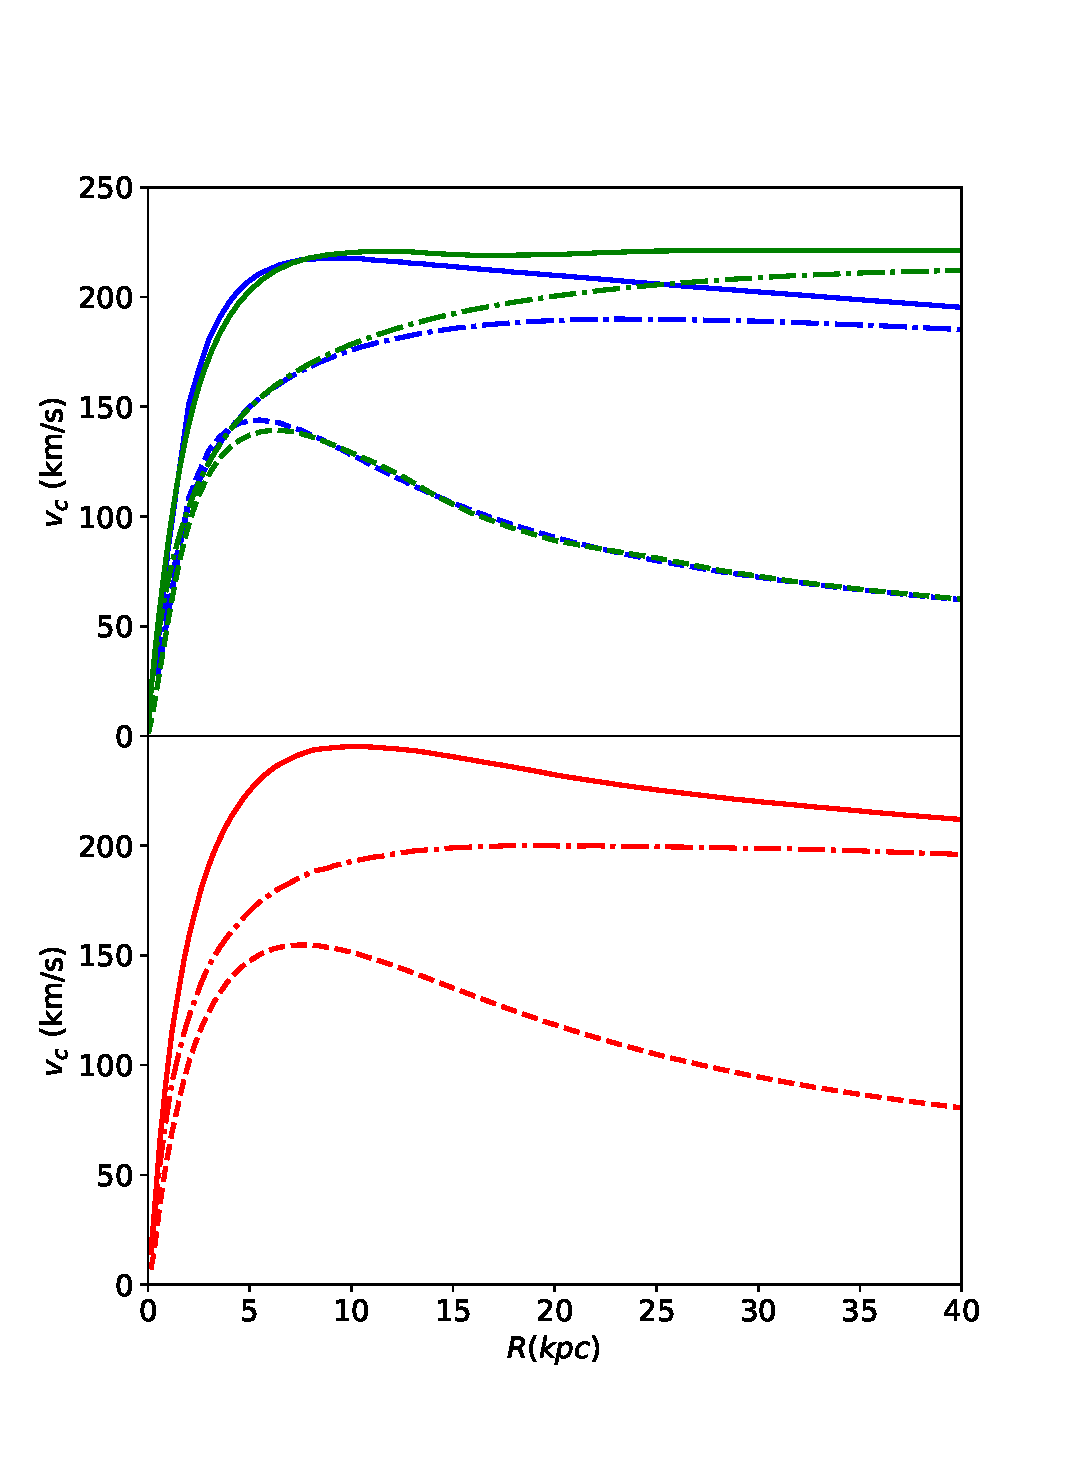
\includegraphics[width=0.8\textwidth]{../figures/rotation_curves_two_panel.eps}
	\caption{Rotation curve decomposition for our models. Total
          rotation curves are shown as solid lines while the separate
          contributions from the disc and halo are shown as dashed and
          dot-dashed curves, respectively.  Blue curves in the top
          panel are for the isolated galaxy simulations with
          \textsc{GalactICS} initial conditions while the green curves
          are for the simulations C.I.Ag run with \textsc{AGAMA}
          initial conditions.  Bottom panel shows initial rotation
          curve decomposition for the runs D.I and
          E.II.}\label{fig:rcs}
\end{figure}


\begin{sidewaystable}
\begin{tabular}{l l l l l l l l l l l l l}
\hline
 & $M_d$ & $R_d$ & $V_c$ & $\sigma_R$ & $z_d/R_d$  & $\sigma_R/\sigma_z$  & $X$ &  $Q$ & $\rho_h/\rho_0$ & $\epsilon$ & {Description}\\ 
\hline
A.I{/A.III}     & 3.49 & 2.50 & 216 & 25.3 & 0.10 & 1.27 & 2.34 & 1.00 & 0.14 & 0.15 & {Thin, Fiducial / Thin, Isotropized}\\
A.II    & 3.49 & 2.50 & 216 & 25.3 & 0.10 & 1.27 & 2.34 & 1.00 & 0.14 & 0.50 & {Thin, High Softening}\\
B.I{/B.III}     & 3.49 & 2.50 & 213 & 25.3 & 0.20 & 0.97 & 2.34 & 1.00 & 0.28 & 0.15 & {Mid, Fiducial / Mid, Isotropized}\\
B.II    & 3.49 & 2.50 & 213 & 25.3 & 0.20 & 0.97 & 2.34 & 1.00 & 0.28 & 0.50 & {Mid, High Softening}\\
C.I     & 3.49 & 2.50 & 208 & 25.3 & 0.40 & 0.77 & 2.34 & 1.00 & 0.50 & 0.15 & {Thick, Fiducial} \\
C.I.Ag  & 3.49 & 2.50 & 216 & 25.3 & 0.40 & 0.77 & 2.34 & 1.00 & 0.50 & 0.15 & {Thick, AGAMA ICs}\\
D.I    & 5.82 & 3.70 & 245 & 25.2 & 0.10 & 1.14 & 2.45 & 1.00 & 0.29 & 0.18  & {Thin, Cosmological}\\
E.II    & 5.82 & 3.70 & 245 & 27.4 & 0.25 & 0.72 & 2.45 & 1.00 & 0.73 & 0.74 & {Thick, High Softening, Cosmological}\\
\hline
YS15.A5 & 5.00 & 3.00 & 263 & 30.7  & 0.2 & 1.00 & 3.22 & 1.38 & 0.21 & 0.68 & {--}\\
YS15.B5 & 5.00 & 3.00 & 211 & 26.6  & 0.2 & 1.00 & 2.06 & 0.96 & 0.11 & 0.68 & {--}\\
YS15.C5 & 5.00 & 3.00 & 270 & 30.3  & 0.2 & 1.00 & 3.31 & 1.42 & 0.23 & 0.68 & {--}\\
YS15.D5 & 5.00 & 3.00 & 236 & 26.6  & 0.2 & 1.00 & 2.58 & 1.12 & 0.16 & 0.68 & {--}\\
YS15.E5 & 5.00 & 3.00 & 233 & 27.1  & 0.2 & 1.00 & 2.58 & 1.11 & 0.15 & 0.68 & {--}\\
YS15.F5 & 5.00 & 3.00 & 219 & 27.0  & 0.2 & 1.00 & 2.22 & 1.02 & 0.11 & 0.68 & {--}\\
YS15.G5 & 5.00 & 3.00 & 227 & 28.2  & 0.2 & 1.00 & 2.45 & 1.09 & 0.13 & 0.68 & {--}\\
YS15.H5 & 5.00 & 3.00 & 244 & 28.6  & 0.2 & 1.00 & 2.85 & 1.21 & 0.16 & 0.68 & {--}\\
\hline
G06     & 7.77 & 5.57 & 226 & 17.1  & 0.06  & 1.80 & 2.78 & 1.43 & 0.10 & 0.15 & {--}\\
\hline
%$M_d$ & $7.2 \times 10^{10} M_\odot$\\
%$N_d$ & $10^6$\\
%$R_{d,0}$ & 3.7 kpc\\
%$N_{r}$ & $4096^3$
\end{tabular}
\caption{Summary of parameters for the simulations considered in this
  paper, the disc-halo simulations considered in
  \citet{YurinSpringelStellarDisks} (labeled YS15) and the
  \citet{gauthier2006} (G06).  $M_d$ is the final disc mass in units of
  $10^{10}\,M_\odot$ , $R_d$ is the disc scale radius in units of
  ${\rm kpc}$, and $V_c$ and $\sigma_R$ are the circular speed and
  radial velocity dispersion in units of ${\rm km\,s^{-1}}$ and
  evaluated at $R_p = 2.2R_d$.  For the disc aspect ratio, we quote
  $z_d/R_d$ where $z_d$ is the ${\rm sech}^2$-scale length.  The
  velocity dispersion ratio $\sigma_R/\sigma_z$, the $X$ and $Q$
  parameters, the ratio of the halo density in the midplane to that of
  the disc, and the logarithmic derivative of the circular speed are
  also measured at $R_p$.  Finally, the softening length $\epsilon$ is
  given in units of ${\rm kpc}$.  Simulations A.III and B.III are the
  same as A.I and B.I except that they are run with vertical motions
  isotropized so as to shut off the buckling
  instability.} \label{tab:sims}
\end{sidewaystable}

\section{Theoretical Considerations}
 \label{sec:ics}

In this section, we consider the structural properties of disc-halo
models with an eye toward understanding the formation of bars in these
systems.  We begin with the $Q$ and $X$ parameters and then discuss the
vertical structure of the disc as defined by its scale height,
vertical velocity dispersion, and surface density.  Finally, we
consider the effect softening might have on bar formation.

\begin{figure}
		\centering
        \includegraphics[width=0.8\textwidth]{../figures/falpha.eps}
        \caption{The dimensionless ratio $\sigma_z^2/\pi G\Sigma z_d$ as a
          function of $\rho_h/\rho_0$ for the models considered in
          this paper (stars), the disc-halo models from
          \citet{YurinSpringelStellarDisks} (filled squares) and the
          model from \citet{gauthier2006} (filled triangle).  The
          straight line is the function $f = 1 + \left (2\pi/3\right
          )^{1/2}\rho_h/\rho_0$ discussed in the text.}
\label{fig:falpha}\end{figure}

\begin{figure}
		\centering
        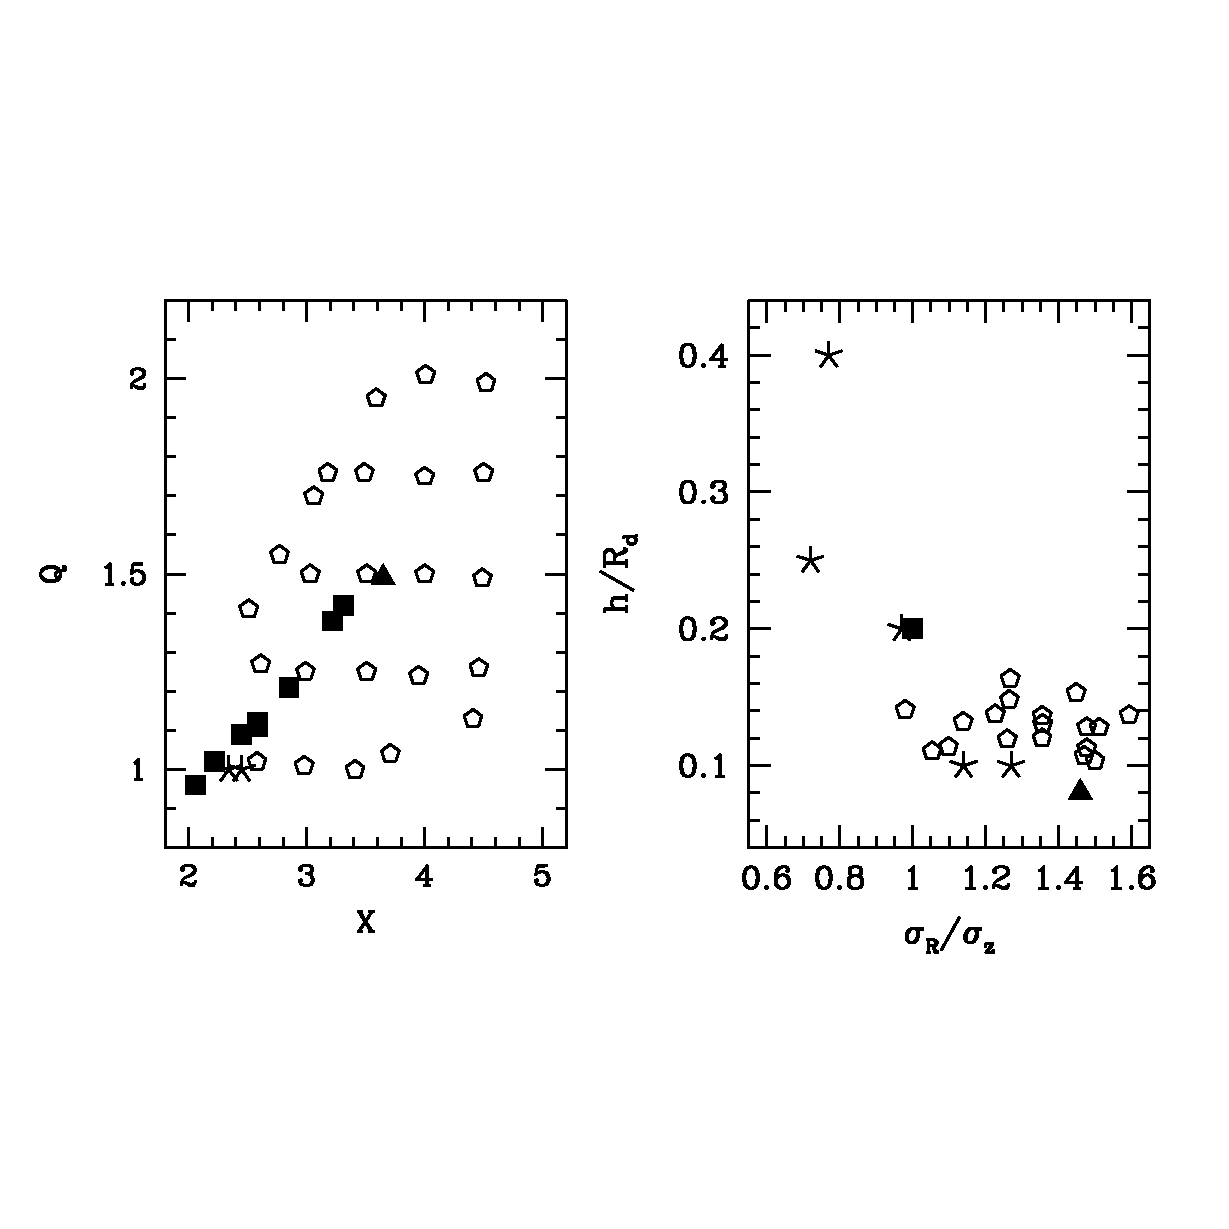
\includegraphics[width=1.\textwidth]{../figures/qxr.eps}
        \caption{Distribution of simulations considered in this paper
          in the $Q-X$ and the $z_d/R_d-\sigma_R/\sigma_z$ planes.
          Stars are simulations run for this paper (A-E); filled
          squares denote the series of simulations described in
          \citet{YurinSpringelStellarDisks}; the filled triangle denotes
          the simulation of M31 run in \citet{gauthier2006}; open
          pentagons denote the simulations described in
          \citet{WPDGalactICSReference}.
        }\label{fig:QXR}\end{figure}


\begin{figure}
	\centering
	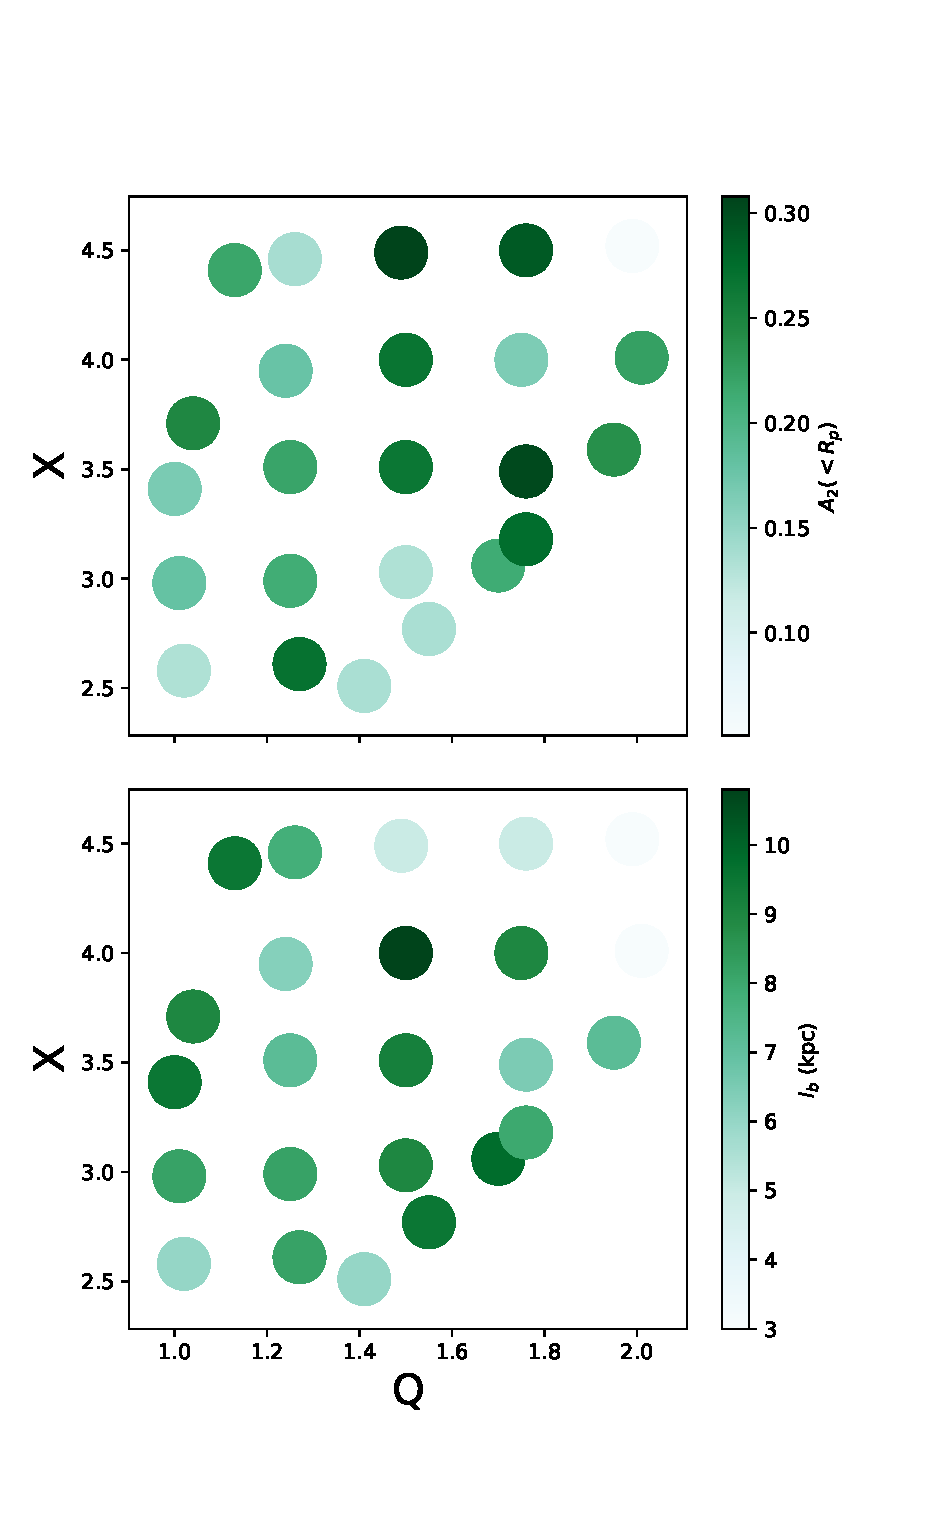
\includegraphics[width=0.8\textwidth]{../figures/wpd.eps}
	\caption{Strength and length of bars for the simulations
          considered in \citet{WPDGalactICSReference}.  The twenty-five models
          span the $Q$-$X$ plane.  Top panel shows the $A_2$ parameter
          while the bottom panel shows the bar length, $l_b$.  Both are
          measured at $5\,{\rm Gyr}$ (the final snapshot of the
          simulations). {The bar length is the full bar length.}}
	\label{fig:qxa2}
\end{figure}


\begin{figure}
	\centering
	\includegraphics[width=\textwidth]{../figures/isolated_xy_with_agama_with_circles.eps}
	\caption{Surface density maps for isolated galaxy simulations
          at select times. Time proceeds from 0 to 10 Gyr,
          left-to-right, and the models span top-to-bottom in order of
          their appearance in Table \ref{tab:sims}. The overlaid red
          circles have radii $R_p=5.5\,{\rm kpc}$ and 20 kpc. {Recall $R_P=2.2 R_d$, the 
          radius of peak circular velocity.}}
	\label{fig:face_on_isolated}
\end{figure}

\begin{figure}
	\centering
	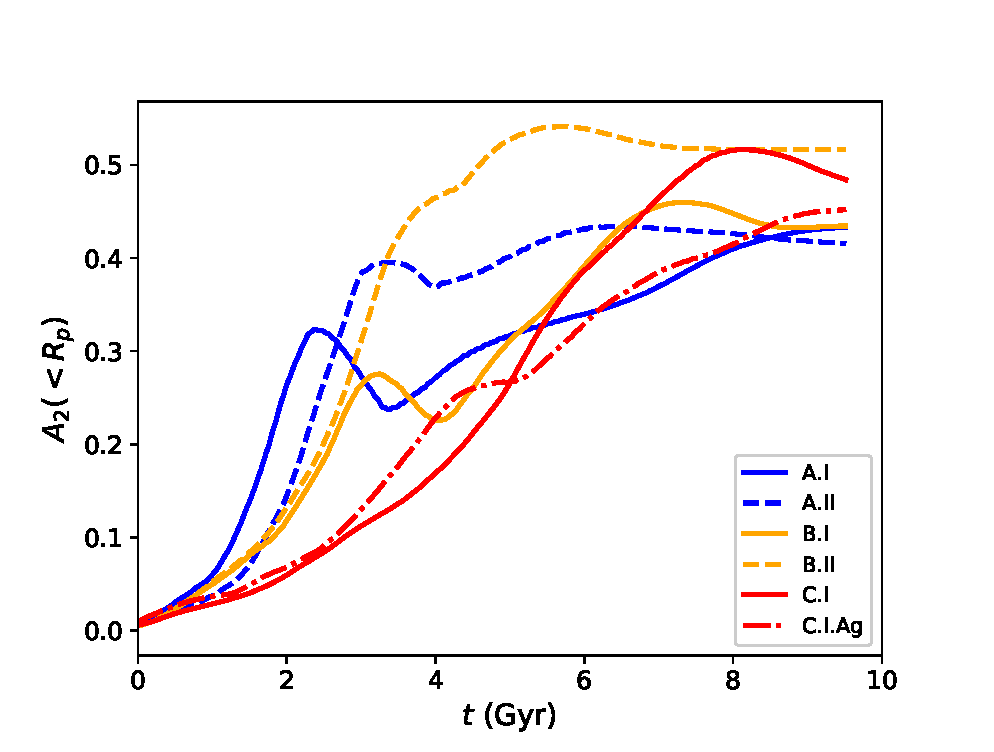
\includegraphics[width=0.8\textwidth]{../figures/isolated_a2_vs_t_2rd_weighted.eps}
	\caption{Mean bar strength parameter inside a cylindrical
          radius $R_p$, $A_2(<R_p)$, as a function of time. Curves are
          smoothed in time with a top-hat moving window of width
          $1\,{\rm Gyr}$.  Line colours are blue, red, and {orange} for
          models A, B, and C, respectively.  Results for the
          fiducial runs A.I, B.I, and C.I are shown as solid curves
          while the results for the runs with high softening length,
          A.II and B.II, are shown as dashed curves.  The
          \textsc{AGAMA} model C.I.Ag is shown as a dot-dashed
          curve.} \label{fig:isolated_a2_vs_t}
\end{figure}

\begin{figure}
	\centering
	\includegraphics[width=1.1\textwidth]{../figures/isolated_r_t_a2_with_agama.eps}
	\caption{Bar strength parameter $A_2$ as a function of radius
          and time.  The trajectory of corotation is shown by the
          dashed red line.} \label{fig:isolated_r_t_a2}
\end{figure}

\begin{figure}
	\centering
	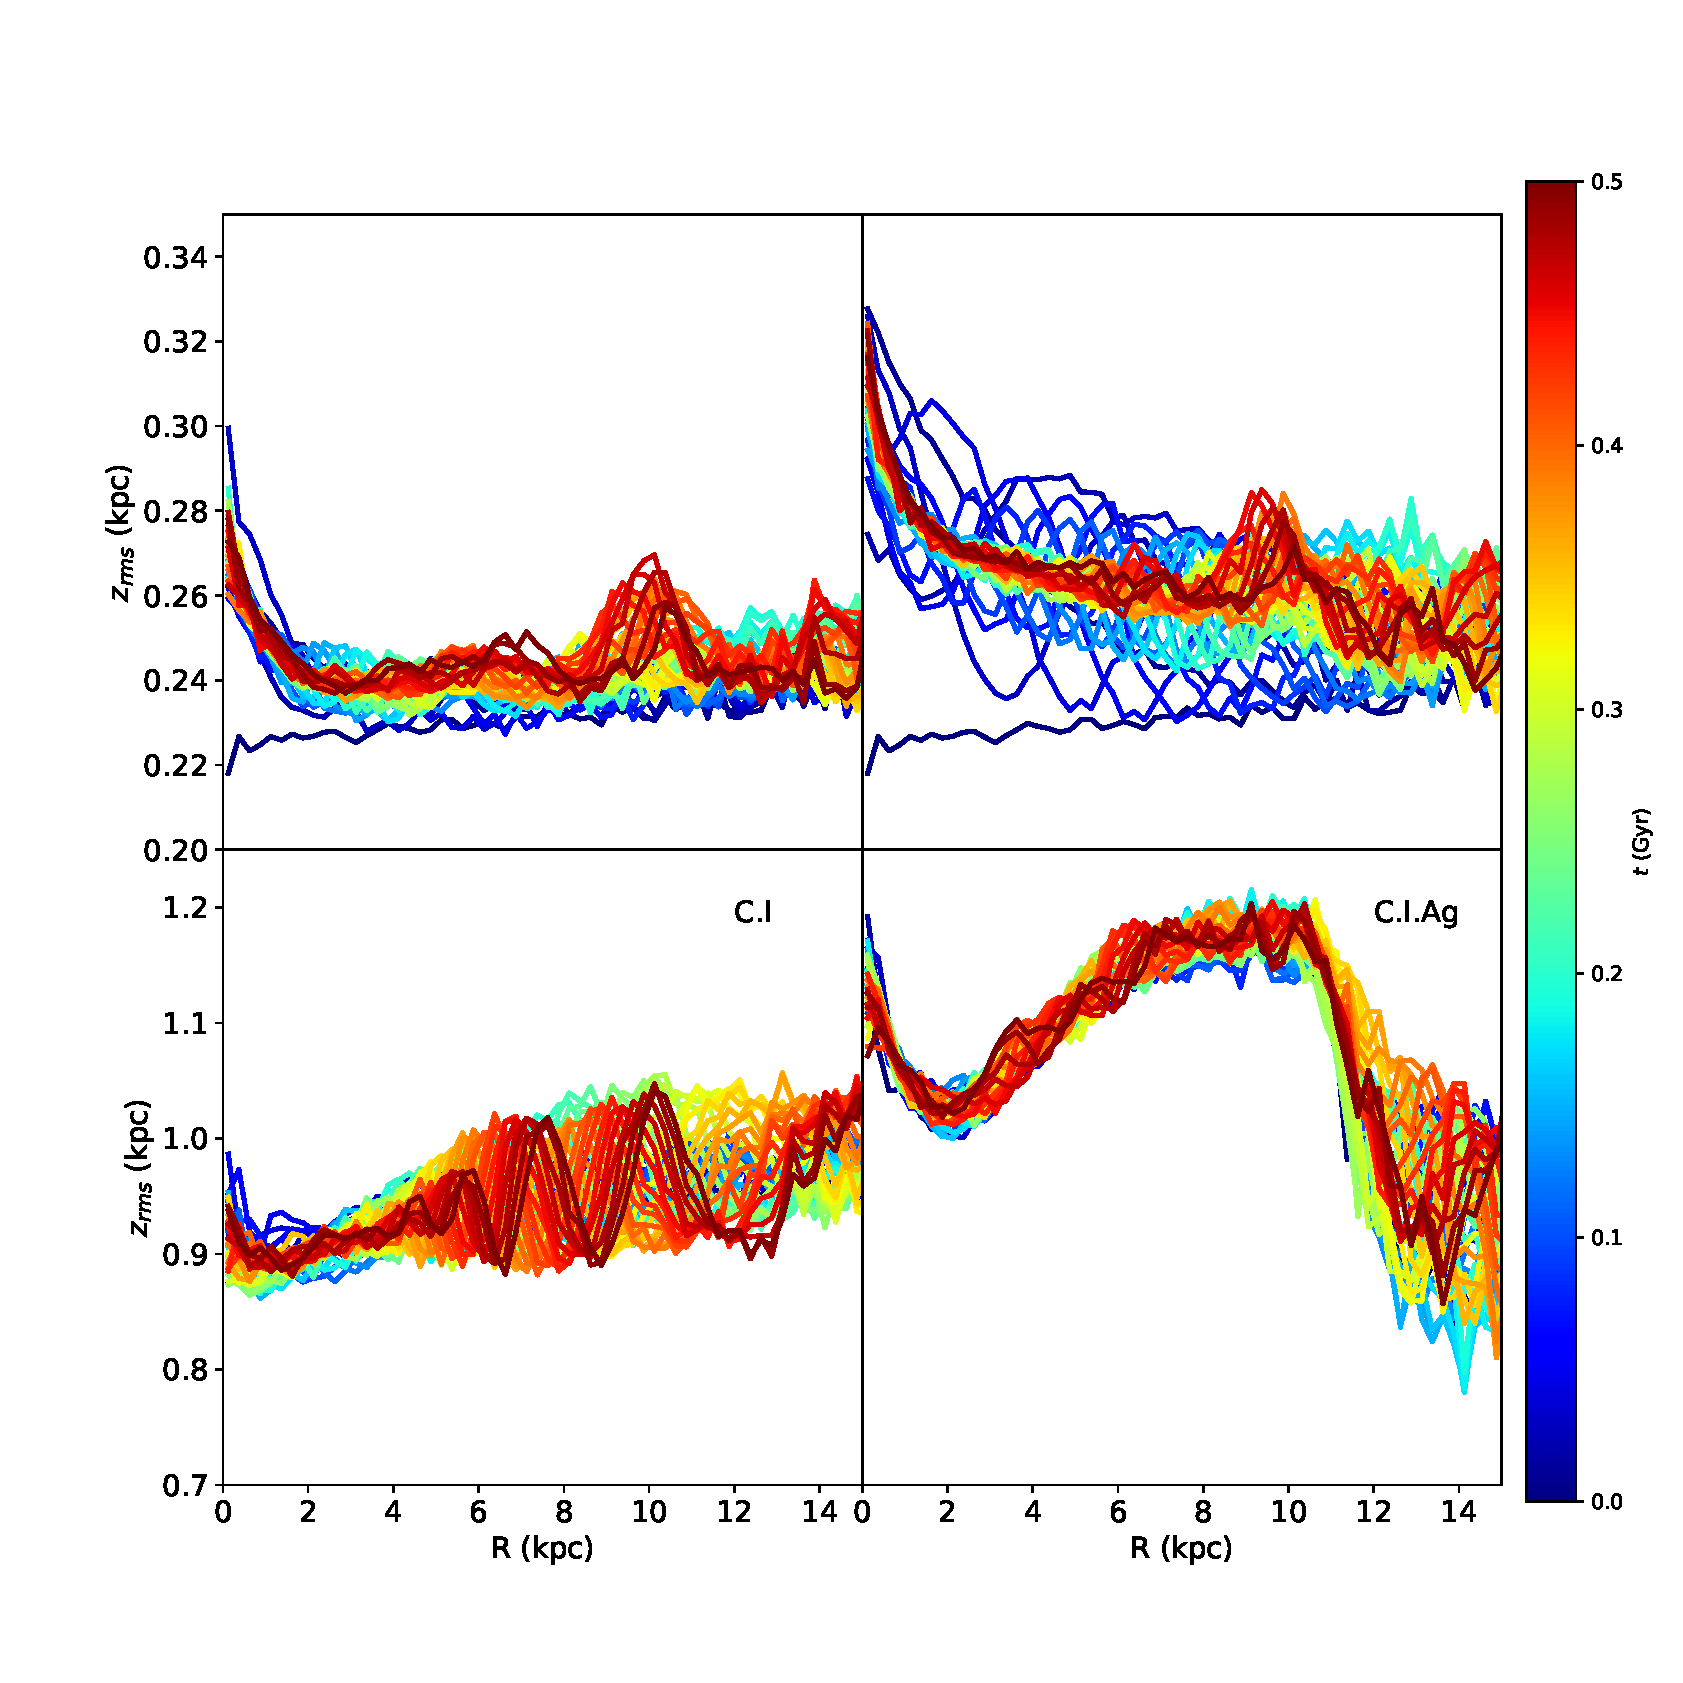
\includegraphics[width=\textwidth]{../figures/isolated_four_panel_zrms.eps}
	\caption{Root mean square height $\zrms$ as a function of
          cylindrical radius $R$ for ten snapshots equally spaced over
          the first $500\,{\rm Myr}$.  Panels are for simulations A.I
          (upper left), A.II (upper right), C.I (lower left) and
          C.I.Ag (lower right).} \label{fig:zrms}
\end{figure}

\begin{figure}
	\centering
	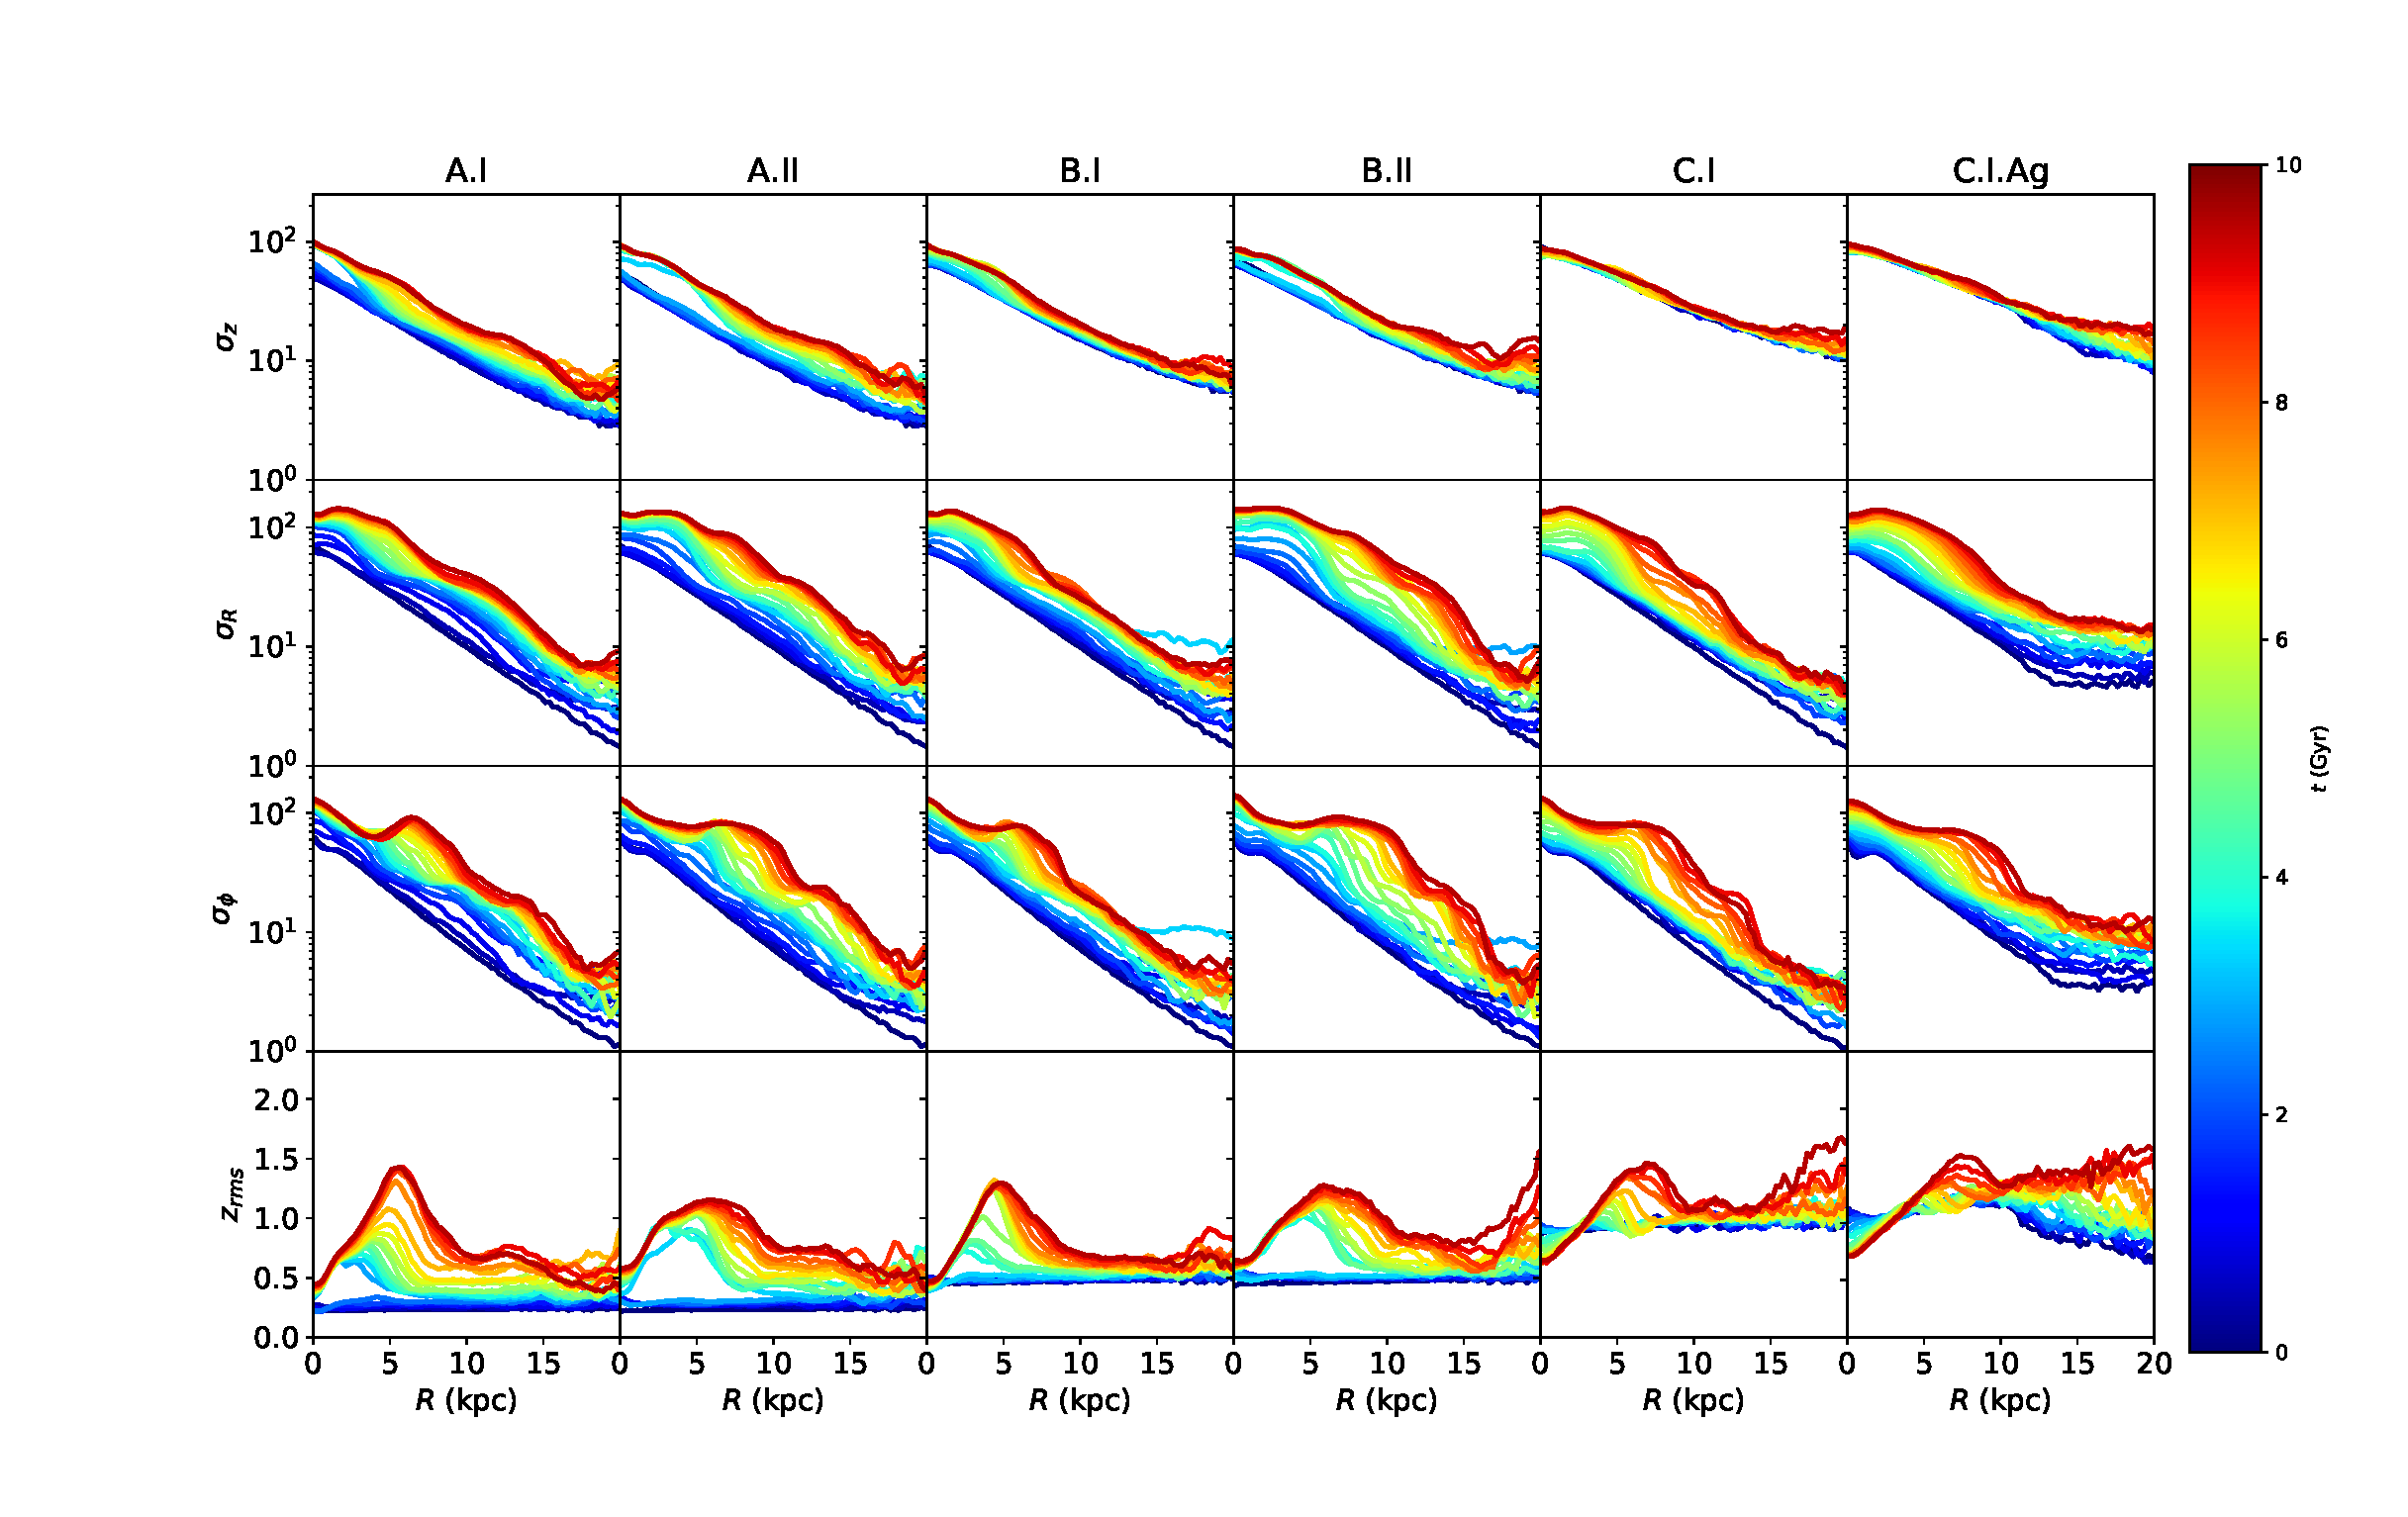
\includegraphics[width=\textwidth]{../figures/isolated_dispersion_evolution_with_agama_zrms.eps}
	\caption{Diagonal components of the velocity dispersion tensor
          and $\zrms$ as a function of $R$ for different snapshots
          between $0$ and $10\,{\rm Gyr}$.  Shown, from to to bottom,
          are profiles for $\zrms$, $\sigma_z$, $\sigma_R$, and $\sigma_\phi$
          for the same size models included in
          Fig.\,\ref{fig:face_on_isolated}.} \label{fig:isolated_dispersions}
\end{figure}

\subsection{$Q$ and $X$} 
The stability of a stellar disc is generally thought to be determined
by the Toomre-$Q$ parameter \citep{ToomreParameter}

\begin{equation} \label{eq:q}
Q \equiv \frac{\sigma_R\kappa}{3.36G\Sigma}
\end{equation}

\noindent and the Goldreich-Tremaine (swing amplification) parameter
\citep{GoldreichTremaine1978, GoldreichTremaine1979}

\begin{equation} \label{eq:xm}
X_m \equiv \frac{\kappa^2 R}{2\pi m G\Sigma}
\end{equation}

\noindent where $R$ is the Galactocentric radius of a cylindrical
$\left (R,\,\phi,\,z\right )$ coordinate system, $\Sigma$ is the
surface density of the disc, $\sigma_R$ is the radial velocity
dispersion of the disc, and $m$ is the azimuthal mode number.  The
epicyclic radial frequency $\kappa$ is given by

\begin{equation} \label{eq:kappa2}
\kappa^2 = \frac{2V_c^2}{R^2}\left (1 + \frac{d\ln{V_c}}{d\ln R}\right )
\end{equation}

\noindent where $V_c$ is the circular speed.  We assume an exponential
disc with mass $M_d$, radial scale length $R_d$, and surface density
\begin{equation} \label{eq:sigma}
\Sigma(R) = \frac{M_d}{2\pi R_d^2} e^{-R/R_d}~.
\end{equation}
\noindent Note that $\kappa$, $\sigma_R$, $\Sigma$, $V_c$, $Q$, and
$X_m$ are functions of $R$.  In what follows, we consider the radius
$R_p$ at which the contribution to the rotation curve from the disc,
$V_d$ reaches a peak value.  For an exponential disc, $R_p \simeq
2.2R_d$ and $V_{d}(R_p) \simeq 0.62 \left (GM_d/R_d\right )^{1/2}$
\citep{BT}.

Roughly speaking, $Q$ describes the susceptibility of a disc to local
instabilities.  Cold discs with low velocity dispersion and $Q<1$ are
unstable to local perturbations.  On the other hand, $X_m$ describes
the vigour with which a global perturbation with an $m$-fold azimuthal
symmetry undergoes swing amplification.  Since we are interested in
bar formation, we set $m=2$ and note that $X_2^{-1}$ is a measure of
disc self-gravity.  To see this, we use Eq.\,(4) and the expression
for $V_{d,p}$ to find

\begin{equation} \label{eq:x2}
X_2(R_p) \simeq  0.79\,\frac{V_c^2}{V_d^2}\Biggr\rvert_{R_p}
\end{equation}

\noindent where we have assumed that the logarithmic derivative in
Eq.\eqref{eq:kappa2} is zero.

For simplicity, we define

\begin{equation} \label{eq:x}
X \equiv  \frac{V_c^2}{V_d^2}\Biggr\rvert_{R_p}~.
\end{equation}

\noindent Therefore $X=2$ when the contribution of the disc to the
circular speed curve at its peak is equal to the combined
contributions of the dynamically hot components, namely the bulge and
halo.  Following \citet{EfstathiouShotNoise},
\citet{YurinSpringelStellarDisks}, use $Q_{\rm bar} = V_{\rm
  max}/\left (GM_d/R_d\right )^{1/2}$ where $V_{\rm max}$ is the
maximum circular speed.  If we assume that $V_{\rm max}\simeq
V_c(R_p)$, then $Q_{\rm bar}^2 \simeq 0.387 X$ and the stability
criterion from \citet{EfstathiouShotNoise}, $Q_{\rm bar}>1.1$, becomes
$X > 3.13$.

\subsection{Vertical Structure of Stellar Discs}

As discussed in \citet{Klypin2009} the vertical structure of a stellar
disc plays a key role in determining the properties of any bar that
forms.  In general, the vertical structure is characterized by the
vertical velocity dispersion $\sigma_z$, surface density $\Sigma$, and
scale height.  For a self-gravitating plane-symmetric isothermal disc
these quantities are connected through the relation $\sigma_z^2 =
\sqrt{12}G\Sigma \zrms$ where $\zrms$ is the root mean square distance
of ``stars'' from the midplane, and $z_d$ is the disc scale height (See
\S\ref{sec:isolated} and 
\citet{spitzer1942, camm1950}).

We can incorporate the effects of dark matter by modifying
the Poisson equation

\begin{equation} \label{eq:spitzerpoisson}
\begin{aligned}
\frac{d^2\Phi}{dz^2} & = 4\pi G \left (\rho_d(z) + \rho_h(z) \right )\\
& = 4\pi G\rho_0 \left(e^{-\Phi/\sigma_z^2} + \rho_h/\rho_0\right )
\end{aligned}
\end{equation}

\noindent where $\rho_d$ and $\rho_h$ are the densities of the disc
and halo, respectively, and $\rho_0$ is the density of the disc in the
midplane.  In the second line we assume, as is done in the pure
self-gravitating case, that the disc stars are vertically isothermal
with velocity dispersion $\sigma_z$.  We also assume that the halo
density is constant in the region of the disc.  We then solve
Eq.\,\ref{eq:spitzerpoisson} numerically.  The result is
well-described by the relation

\begin{equation}\label{eq:sigz2}
\sigma_z^2 = \sqrt{12} 
G\Sigma \zrms \left (1 + \alpha\rho_h/\rho_0\right )
\end{equation}

\noindent where the factor $\alpha = \sqrt{2\pi/3}$ provides a
simple interpolation between the pure self-gravitating case and the
case where disc particles are test particles in the (harmonic)
potential of a constant density halo.  {We plot the simulations to 
be presented in this paper, along with others, in Fig. \ref{fig:falpha}.
We see variation about a line with slope $\alpha$ of the simulations
detailed in Table \ref{tab:sims}. Simulations deviate from this trendline
substantially as the disc scale height is increased and the planar model
we considered becomes less accurate.}

As discussed in the next
section Eq.\,\ref{eq:sigz2} holds at the 10 per cent level for our
equilibrium models.  Departures from Eq.\,\ref{eq:sigz2} might come
from radial gradients and the rotation of the disc. (See, for example,
\citet{read2014}).

Combining Eqs.\,\ref{eq:q}, \ref{eq:x}, \ref{eq:sigz2} we find 
following relation:

\begin{equation}\label{eq:r}
\frac{Q^2}{X} = 3.103 \,
\frac{\sigma_R^2}{\sigma_z^2} \,
\frac{\zrms}{R_d}\,
f\left (1 + \frac{d\ln V_c}{d\ln R}\right )~.
\end{equation}
\noindent This expression can be interpreted in several ways.  First,
if the ratios of $\sigma_R$ to $\sigma_z$ and $\zrms$ to $R_d$ are
fixed, then there is a linear relation between $Q^2$ and $X$.  On the
other hand, if one considers a family of models in which the only
variation is in the vertical structure of the disc, then the scale
height varies roughly linearly with the vertical velocity dispersion,
apart from corrections due to the contribution of the halo to the
vertical force.

\subsection{Effect of Gravitational Softening} 

Numerical effects can significantly alter the development of bars in
simulated galaxies. For example, in simulations of an isolated galaxy
that is initially in equilibrium, the onset of bar formation is
delayed when mass resolution is increased \citep{dbs2009}
essentially because the bar instability is seeded by shot noise.  The
importance of mass resolution as well as force resolution and time
stepping have been discussed in \citet{Klypin2009}.

In this section, we focus on the effects of force softening. {Gravitational
softening is necessary to avoid large (possibly infinite) forces that arise
from Newtonian two-body interactions. }
Equilibrium models, such as the ones used as initial conditions in
isolated galaxy simulations, satisfy the collisionless Boltzmann and
Poisson equations.  When evolved with force softening, they will begin
slightly out of equilibrium.  This effect should be most noticeable
when the softening length is comparable to or larger than the
thickness of the disc. {Detailed discussions of the 
effect softened gravity has on the secular evolution of N-body galaxies can be found in
\citet{romeo_1994,AthanassoulaSellwood1986,merritt_1996,weinberg_1996, romeo_1997, romeo_1998}.}

To gain some intuition as to this extent of
this effect we the Poisson equation in one dimension.  The potential
for a mass distribution with vertical density profile of $\rho(z)$ can
be calculated by convolving $\rho$ with the Green's function:
\begin{equation}\label{eq:greensfunction}
\Phi(z)= 4\pi G\int_{-\infty}^{\infty} \mathcal{G}(z^\prime - z)
\rho(z^\prime) \text{d} z^\prime~.
\end{equation}
For Newtonian gravity, $\mathcal{G} = |z|/2$.  For softened gravity,
we replace $\mathcal{G}$ with $\mathcal{G}_s = \frac{1}{2}\left (z^2 +
\epsilon^2\right )^{1/2}$ where $\epsilon$ is the softening length.
(The motivation for this expression is as follows: Begin with a system
of Plummer-softened particles, that is, a system where point-like
particles are replaced by particles whose spherical density profile is
proportional to $\left (r^2 + \epsilon^2\right )^{-5/2}$.  If the
particles are confined to a plane, then the vertical density profile
will be $\rho(z)\propto \left (z^2 + \epsilon^2\right )^{-3/2}$.  The
one-dimensional potential with this $\rho(z)$ is indeed proportional
to $\left (z^2 + \epsilon^2\right )^{1/2}$.)  The integral
Eq.\,\ref{eq:greensfunction} and the related integral for the vertical
force, $f(z)$, can be evaluated numerically.  As expected, the
potential energy per unit area of the system, $W \equiv \int
dz\,\rho(z) z f(z)$ is smaller than that of the same system found
assuming Newtonian gravity.  Hence, a system that is set up to be in
equilibrium under the assumption of Newtonian gravity, will be too
``warm'' for a softened gravity simulation and will ``puff up''.  To
an excellent approximation, we find that the virial ratio between the
kinetic energy per unit area and $W$ is given by $2T/W \simeq (1 +
(a\epsilon/\zrms)^2)^{b}$ where $a = 1.25$ and $b = 0.25$.  Roughly
speaking, simulations run with a softening length equal to $\zrms$
will have a virial ratio of $1.25$.

Softening may have other effects on the development of the bar.  In
principle, softening should suppress the Toomre instability on small
scales.  However, this instability develops on scales comparable to or
larger than the Jeans length, which is typically much larger than the
thickness of the disc and hence larger than the softening length for
most simulations.  On the other hand, softening may suppress buckling,
a bending instability, which is strongest on small scales.  As
discussed below, buckling appears to be responsible for regulating the
growth of bars.

\section{Models and Simulations} \label{sec:thick_discs_suppress}

\subsection{Initial Conditions for Isolated Galaxy Simulations} \label{sssec:isolated}

We follow the evolution of isolated disc-halo systems using the N-body
code \textsc{gadget-3} \citep{GadgetCodePaper}.  The initial
conditions for most of our isolated galaxy simulations are generated
with \textsc{GalactICS} \citep{GalactICS1995,WPDGalactICSReference},
which allows users to build multicomponent, axisymmetric equilibrium
systems with prescribed structural and kinematic properties.  Disc
particles are sampled from a distribution function (DF) that is a
semi-analytic function of the total energy $E$, the angular momentum
about the disc symmetry axis $L_z$, and the vertical energy {$E_z = \Phi(R,0) - \Phi(R,z) + \frac{1}{2} v_z^2$, where $\Phi$ is the gravitational potential and $v_z$ is an orbit's vertical velocity. } By
design, the disc DF yields a density law in cylindrical $\left
(R,\,\phi,\,z\right )$ coordinates given, to a good approximation, by
$\rho(R,z) = \Sigma(R)\,{\rm sech}^2(z/z_d)$.  Here $\Sigma(R)$ is
exponential surface density profile (Eq.\,\ref{eq:sigma}) and $z_d$ is
the scale height. Note that $\zrms = \pi/\sqrt{12} z_d$ while the
``half-mass'' scale height used in \citet{YurinSpringelStellarDisks}
is given by $z_{1/2} \simeq 0.549z_d \simeq 0.605 \zrms$.  The disc DF
is also constructed to yield a radial velocity dispersion profile that
is exponential in $R$ with scale length $2R_d$. The halo DF is
designed to yield a truncated NFW profile \citep{NFW} as described in
\citet{WPDGalactICSReference}.

While $E_z$ used in the \textsc{GalactICS} disc DF
is conserved to a good approximation for nearly circular orbits it
varies considerable for stars that make large excursions in $R$ and
$z$.  Thus, the initial conditions for ``thick'' or ``warm'' discs
will not represent true equilibrium solutions to the dynamical
equations.  To test whether non-conservation of vertical energy
affects our results, we compare a thick disc model with
\textsc{GalactICS} initial conditions with a similar one where the
initial conditions are generated with \textsc{AGAMA} \citep{agama}, 
{an action-based code that does not rely on the epicycle 
approximation.  \textsc{AGAMA} initial conditions should be closer 
to the true equilibrium than \textsc{GalactICS} models, especially for the thick discs.}
%{Since
%\textsc{AGAMA} generates its initial conditions from functions of the 
%\textit{actions}, and does not assume the epicycle approximation.}
In principle, this action-based code should yield initial conditions
that are closer to a true equilibrium system than ones based on $E_z$
especially for thick discs.

\subsection{Description of Simulations}

In this section, we describe a suite of simulations where $Q$ and $X$
are fixed and where the velocity dispersion and scale length
ratios are allowed to vary.  Our aim is to test the hypothesis that scale
height plays a key role in the development of bars.  The parameters
for our simulations are summarized in Table \ref{tab:sims}.  Our suite
of isolated galaxy simulations form a sequence A, B, C in increasing
thickness.  The models have the same rotation curve decomposition,
which is shown in the top panel of Fig. \ref{fig:rcs}.  By design, the
contribution to the rotation curve from the disc is slightly below
that of the halo at $R_p$.  Therefore our models have $X$ slightly
greater than $2$ and should be susceptible to global instabilities.

The fiducial simulations are run with a softening length of
$184,\,{\rm pc}$, which is about two thirds of the scale height of our
thinnest model (A.I).  The simulations A.II and B.II use a softening
length of $736\,{\rm pc}$, which is close to the value assumed in
\citet{YurinSpringelStellarDisks}.  The simulation C.I.Ag is similar
to C.I (large scale height) but run with \textsc{AGAMA} initial
conditions.  A comparison of its rotation curve decomposition with
that for model C.I is shown in the top panel of Fig. \ref{fig:rcs}.
The contributions from the discs in the two models are nearly the same
and the contributions from the haloes differ significantly only beyond
$\sim 10\,{\rm kpc}$.  The simulations A.III and B.III use a scheme to
isotropize vertical motions and effectively shut off buckling and are
discussed in \S \ref{sec:buckling}.

In addition to these isolated galaxy simulations we run two
cosmological simulations using the disc insertion scheme described in
\citet{Bauer2018a}.  The initial conditions for these models, labeled
D.I and E.II, are identical except for the vertical scale height and
softening length, which are larger in E.II.  Thus, these models are
cosmological analogs to A.I and B.II.  The rotation curves for these
models are shown in the bottom panel of Fig. \ref{fig:rcs}.  The
models themselves are discussed in Section \S \ref{sec:cosmo}.

\subsection{Comparison with Previous Work}

While the parameters $Q$ and $X$ allow one to predict the rapidity and
vigour with which instabilities develop in disc galaxies that are
actually imperfect predictors of the strength and length of bars at
late times.  The point is illustrated in \citet{WPDGalactICSReference}
where results for a suite of 25 simulations that explore the $Q-X$
plane are presented.  By design, the initial conditions for the models
satisfy observational constraints for the Milky Way such as the
rotation curve, the local vertical force, and the velocity dispersion
toward the bulge.  (See \citet{hartmann2014} for a further analysis of
these simulations.)  As expected, the onset of the bar instability is
delayed in models with large initial values for $Q$ and/or $X$.
However, the dependence on these parameters of the bar strength and
length is more complicated.  {In Fig. \ref{fig:QXR}, we show the distribution
of models  in the $Q-X$ and $z_d/R_d-\sigma_R/\sigma_z$ planes from a few papers which
 consider Milky Way like galaxies.
It is common for bar formation studies to consider only a small subset
of the total parameter space. As we will see, models which are close together
in $Q$ and $X$ may exhibit very different bar formation behaviour.}

In Fig.\ref{fig:qxa2}, we show the bar
strength parameter $A_2$ and length of the bar { across the models considered
in \citet{WPDGalactICSReference}.}
Evidently, the models that form the strongest and longest bars have
intermediate values of $Q$ and $X$.  The implication is that models
where the instabilities grow too quickly lead to weaker and somewhat
shorter bars.  Bar formation appears to be a self-regulating process.

Table \ref{tab:sims} gives the relevant parameters for the eight
disc-halo models from \citet{YurinSpringelStellarDisks} as well as the
disc-bulge-halo model for M31 from \citet{gauthier2006}.  In the
\citet{YurinSpringelStellarDisks} simulations discs are inserted into
dark matter haloes from the cosmological Aquarius simulation.  In this
respect, they are similar to the disc-insertion simulations described
in Section \S \ref{sec:cosmo}.  The initial discs in these models all
have a scale height to scale length ratio of $0.2$ and a radial to
vertical velocity dispersion ratio of $1$.  As discussed above, these
choices mean that their discs were chosen from a one-parameter family
of models within the $Q-X$ parameter space.

\section{Isolated Galaxy Simulations}\label{sec:isolated}

\subsection{Morphology of Bar Forming Galaxies}

Face on surface density maps for models A.I, A.II, B.I, B.II, C.I, and
C.I.Ag are shown in Fig.\,\ref{fig:face_on_isolated}.  All discs form
bars by the end of the simulation ($t=10\,{\rm Gyr}$).  However, bar
formation appears to be delayed in models B.I and C.I relative to that
in model A.I while the final bar in A.I is shorter than those in B.I
and C.I.  Other $m=2$ features are also evident.  These include
two-armed spiral structure, most clearly seen in A.I and B.III and
elliptical rings, as, for example, in C.I.

Evidently, the dominant mode for in-plane perturbations is $m=2$
Nevertheless, there are strong $m=3$ structures in the $1.5\,{\rm
  Gyr}$ snapshot of the A.I and A.II simulations and hints of a weak
$m=3$ structure in the same snapshot of B.II.

A larger softening length seems to lead to stronger bars at
intermediate times.  We see this in the comparison of A.I and A.II or
B.I and B.II in the $3.0\,{\rm Gyr}$ and $4.5\,{\rm Gyr}$ snapshots.

\subsection{Bar Strength Parameter $A_2$}

It is convenient to think of the azimuthal distribution of particles
in a given radial bin as a Fourier series.  {We use the canonical definition for the coefficient
of the Fourier component with $m$-fold azimuthal symmetry (see \citet{debattista_sellwood_2000}, for instance),}
\begin{equation}\label{eq:cm}
c_m =  \frac{1}{M_S} \sum_{j \in S} \mu_i e^{i m \phi}
\end{equation}

\noindent {where $\mu_i$ is the mass of the $i$-th particle, $S$ is
a circularly symmetric region of the disc, and $M_S$ is the mass in this region. }
The normalization is
chosen so that a distribution of particles along a line through the
origin will have $|c_m|=1$ for all $m$ even.  Moreover, for a uniform
distribution of particles, $c_0=1$ and $c_m=0$ for all $m>0$.  The
amplitude and phase for the $m$-th Fourier coefficient are given by
$A_m \equiv \vert c_m \vert$ and $\phi_m = \text{arg } (c_m)$,
respectively.  Note that both of these quantities depend on the region
$S$

Fig. \ref{fig:isolated_a2_vs_t} shows a plot of the mean $A_2$ inside
the radius $R_p$ as a function of time for the fiducial simulations,
the two simulations with high softening, and the thick disc simulation
with initial conditions from \textsc{agama}.  Consider first the
fiducial (low-softening) simulations.  Initially, $A_2$ grows roughly
exponentially with a growth rate that decreases with increasing
thickness.  In simulations A.I and B.I, the end of exponential growth
is followed by a decrease in $A_2$ after which $A_2$ again increases,
now, approximately linearly with time.  In the thick disc case (C.I)
exponential growth transitions directly to linear growth.  The trend
is for exponential growth to end at later times as one goes to thicker
discs.  It is worth noting that the value of $A_2$ at $10\,{\rm Gyr}$
is similar in the three low-softening simulations.

In the thin disc case, an increase in softening appears to delay the
onset of exponential growth as well as the time at which exponential
growth ends.  Furthermore, the drop in $A_2$ is less severe.  Though
the value of $A_2$ at the end of the simulation is approximately the
same in the low and high softening cases, the bar strength, as
measured by $A_2$ is larger in the high-softening case at intermediate
times between $4$ and $8\,{\rm Gyr}$.  For the intermediate thickness
case (B.I and B.II) softening has little effect on the initial
growth rate of $A_2$.  But as in the thin disc case, softening
allows exponential growth to continue to later times and the final bar
is about twenty per cent stronger as compared with the low-softening
case.  Once again we see that the effect of high softening is to
produce stronger bars at intermediate times.

The evolution of $A_2$ for the thick disc runs with \textsc{GalactICS}
and \textsc{agama} initial conditions are fairly similar.  In particular,
the initial growth rate is almost identical as are the final values.

Fig. \ref{fig:isolated_a2_vs_t} encapsulates bar strength into a
single number, the mean $m=2$ Fourier amplitude inside $2.2$ disc
scale lengths, or about $5.5\,{\rm kpc}$.  A more complete picture of
bar strength is presented in Fig.\,\ref{fig:isolated_r_t_a2} where we
plot $A_2$ as a function of $R$ and $t$. The figure is constructed by
calculating $c_2$ (Eq.\,\ref{eq:cm}) for cylindrical rings of radius
$200\,{\rm pc}$.  Also shown is the corotation radius, which is
determined from the pattern speed $\Omega_p$ and rotation curve. The
former is given by a numerical estimate of ${\text{d}
  \phi_2}/{\text{d} t}$; corotation is found by determining the radius
at which $\Omega_p = V_c/R$.  Thus, since our galaxy models have
roughly flat rotation curves beyond $5\,{\rm kpc}$, the corotation
essentially gives the inverse pattern speed or pattern period.

From {Fig. \ref{fig:isolated_r_t_a2}} we see that the corotation radius
tends to grow with time and provides an envelope for the bar and other
$m=2$ structures such as two-armed spirals and elliptical rings.  The
bar pattern speed is therefore decreasing with time, presumably due to
dynamical friction between the bar and both the disc and dark halo
\citep{debattista1998, debattista2000}.  It is worth noting that the
corotation radius increases more rapidly in simulations with high
softening.  The naive interpretation is that softening somehow
increases the frictional coupling between the bar and disc or halo
particles.  A more likely explanation is that with a high softening
length comes stronger bars.  Since the acceleration on the bar due to
dynamical friction scales as the mass of the bar, stronger bars should
spin down more rapidly.

As in Fig. \ref{fig:isolated_a2_vs_t} we see that bar formation
is delayed in models with thicker discs.  Bar formation is 
well underway by $2\,{\rm Gyr}$ in A.I but doesn't really take hold
until $4\,{\rm Gyr}$ in C.I.  Moreover, the first hints of $m=2$ power
in C.I arise further out at radii closer to $5\,{\rm kpc}$.  

The dip in bar strength is clearly seen between $2.5-3\,{\rm Gyr}$ in
A.I and between $3.5-4\,{\rm Gyr}$ in B.I.  As discussed below, we
attribute this dip to buckling.

\subsection{Vertical Structure and Velocity Dispersion}

%Figs.\,\ref{fig:zrms} and \ref{fig:isolated_dispersions} show the
%$\zrms$ and velocity dispersion profiles for a sequence of snapshots
%in various models.  

{Fig.\,\ref{fig:zrms} shows the
$\zrms$ radial profiles for a sequence of snapshots
in various models.  
The  evolution
of $\zrms$ is studied during the initial $500\,{\rm Myr}$ of the simulation.  The
top panels show the $\zrms$ profiles for simulations A.I and A.II and
illustrate the effect softening has on the evolution from
``equilibrium'' initial conditions.  As discussed in \S2,} a
system that is initialized to be in equilibrium under the assumption
of Newtonian gravity will be out of equilibrium if evolved with
softened gravity.  In particular, the mean potential energy will be
systematically low and the system will puff up.  For our thin disc
model, $\zrms\simeq 230\,{\rm pc}$.  In the high softening case,
$\epsilon = 736\,{\rm pc} \simeq 2.2\zrms$, we estimate the virial ratio
for the vertical structure to be $2T/W\simeq 1.7$.  Of course, the
excess kinetic energy will redistribute itself into both kinetic and
potential energy.  The upshot is that the system quickly settles into
a new state with a thickness somewhat larger than the initial one as
seen in the right hand panel. {One might be tempted to suggest
that a high softening implies that a disc behaves like a thicker disc.
This picture is not quite correct, since a thicker disc will not 
substantially redistribute energy if it is initialized in equilibrium.}

The bottom panels in Fig.\,\ref{fig:zrms} provide a comparison of
$\zrms$ profiles for the thick disc simulations with
\textsc{GalactICS} and \textsc{agama} initial conditions.  We first
note that $\zrms$ is approximately constant in the C.I but varies by
about $200\,{\rm pc}$ in C.I.Ag.  This difference is simply a
reflection in how the initial conditions are set up.  In both cases,
the scale height depends implicitly on the functional form of the DFs,
which are written in terms of either $E,\,E_z,\,$ and $L_z$ or the
actions.  The \textsc{GalactICS} case does exhibit transient wavelike
perturbations with a peak to trough amplitude of $100\,{\rm pc}$ at
radii $R>4\,{\rm kpc}$.  A plausible explanation for these
oscillations is that they are due to the fact that $E_z$ is not a true
constant of motion.  In any case, the system quickly settles to to a
new equilibrium state not too different from the initial one.


\begin{figure}
\centering
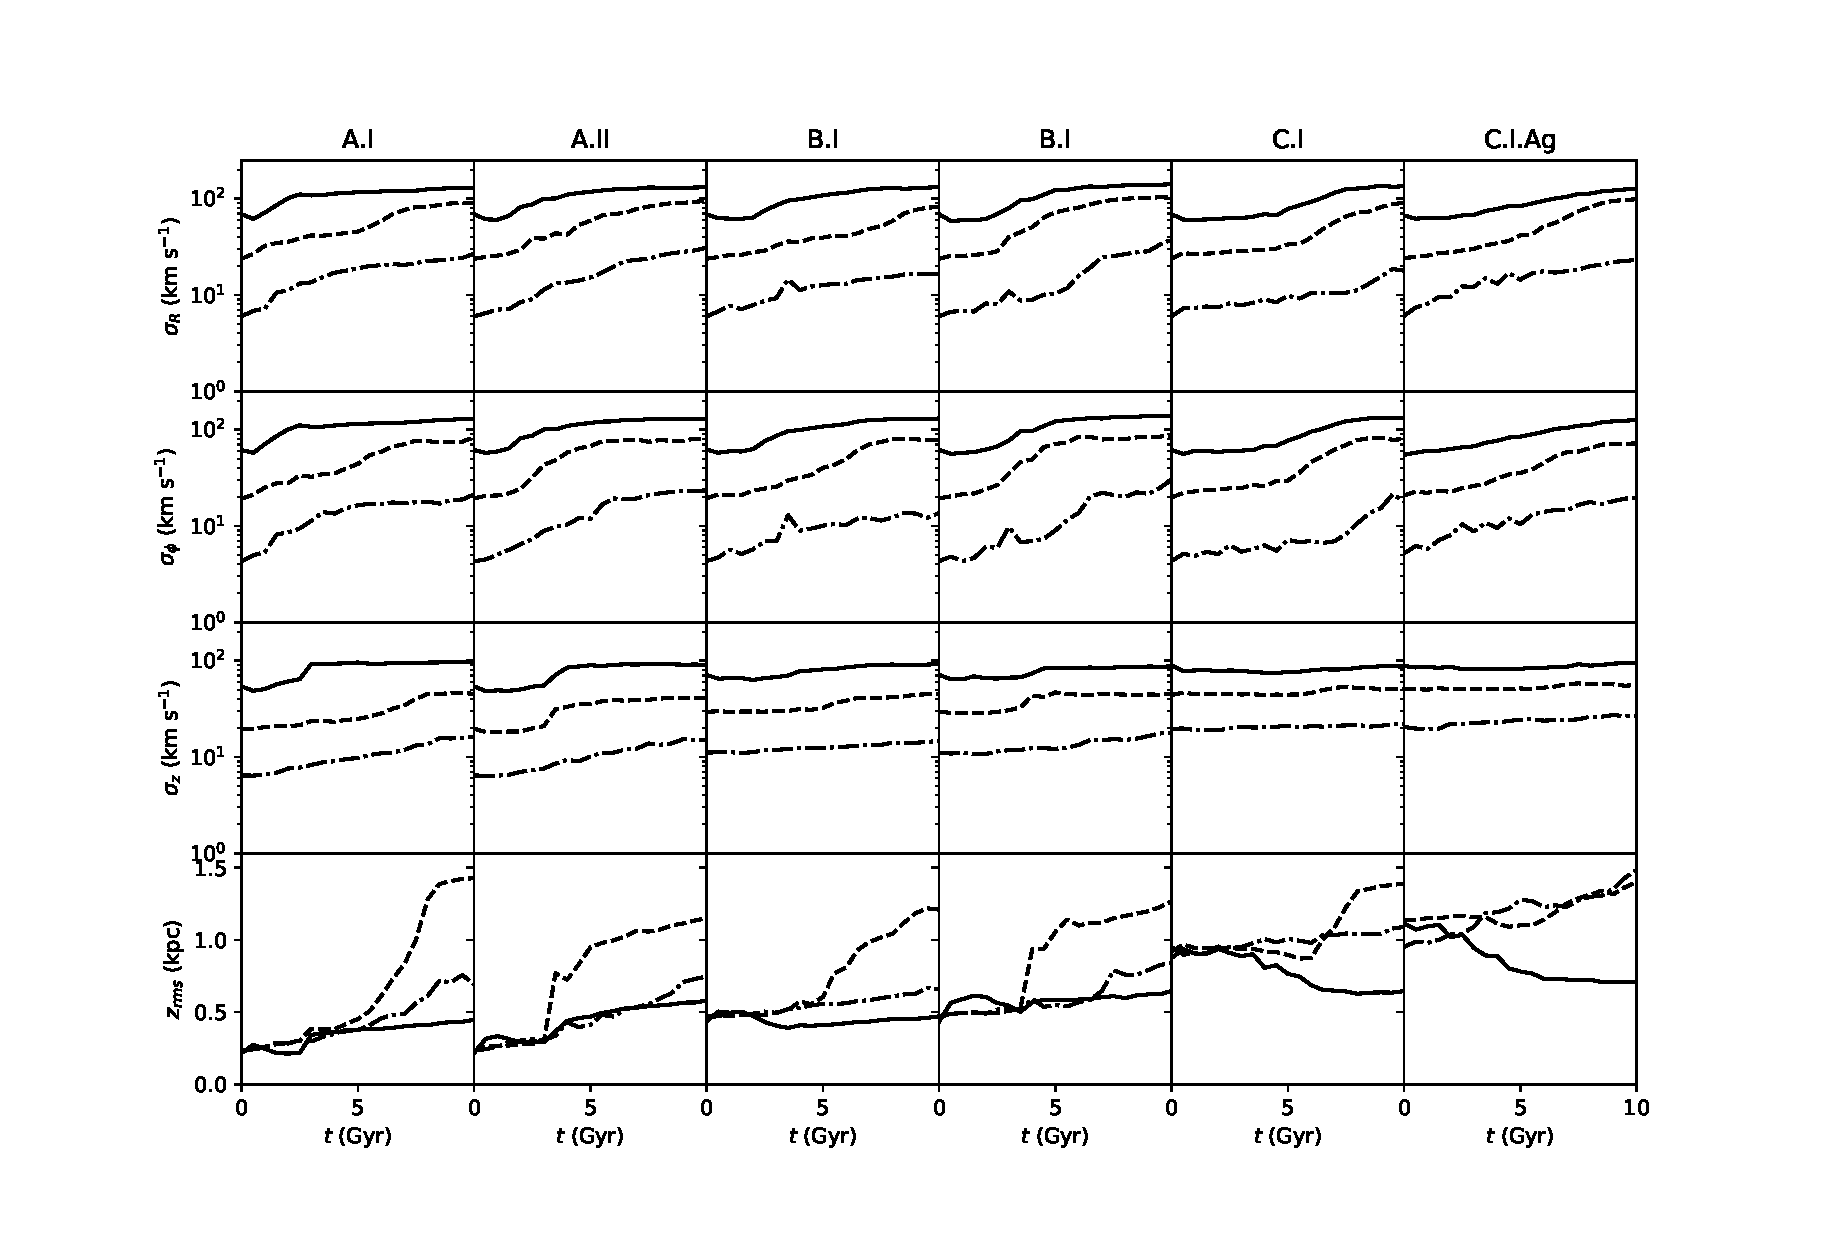
\includegraphics[width=0.9\textwidth]{../figures/dispersions_vs_time.eps}
\caption{The velocity dispersions, $\sigma_R$, $\sigma_\phi$, and $\sigma_z$, and $z_{rms}$
as a function of time for our six fiducial models. The lines are averaged in the circular region
of radius 0.25 kpc (solid), an annulus of width 0.25 kpc centered near 2.2 $R_d$ (dashed),
and a 0.25 kpc width annulus centered at around 5 $R_d$ (dot-dashed). } \label{fig:dispersions_vs_time}
\end{figure}


Fig.\,\ref{fig:isolated_dispersions} shows profiles for $z_{rms}$ and the
diagonal components of the velocity dispersion tensor, $\sigma_z$,
$\sigma_R$, and $\sigma_\phi$.
{All models exhibit
significant in-plane heating across the disc and throughout the
simulations. While the initial radial velocity dispersion profiles are
exponential in $R$ the final profiles are relatively flat within the central 5
kpc. Thus, the greatest increase in radial velocity dispersion is at
about this radius, which corresponds to the end of the bar. Likewise
the $\sigma_\phi$ profile develops a ``bump" around
$R\simeq 5-10$ kpc.}

%{The $\sigma_R$ and $\sigma_\phi$ components
%heat substantially in all models. The $\sigma_z$ profile heats in the thinner 
%discs, but remains relatively constant in C.I and C.I.Ag. While vertical heating occurs
%relatively uniformly, the cylindrically averaged $\sigma_R$ and $\sigma_\phi$ have
%characteristic non-uniformity around the region of the bar. This is also reflected
%%in the $z_{rms}$ profiles as a function of radius. Strangely, the disc cools vertically
%in the thicker models. This latter effect is clearer
%in Fig. \ref{fig:dispersions_vs_time} which plots the dispersions and $z_{rms}$
%at several radii against time. A decreasing slope in the central $z_{rms}$ is 
%obvious in C.I and C.I.Ag. The vertical dispersion remains roughly
%constant while the other components heat up. }

{Vertical heating and thickening also appear to be connected with
bar formation.  The $\sigma_z$ profile increases in the A.I/A.II and B.I/B.II simulations such
that by 10 Gyr, the central value is ~ 100 km/s. This value is roughly
equal to the initial value in the C.I and C.I.Ag (thick disc)
simulations. Note as well that vertical heating in the inner disc
occurs rapidly beginning around 3-4 Gyr, roughly when the bar
is forming. By contrast, vertical heating of the outer disc occurs
gradually over the entire simulation.}


{The bottom row in Fig. \ref{fig:isolated_dispersions} shows the $z_{rms}$ profiles for the different
simulations. Again, we see that the inner disc in the A.I/A.II and B.I/B.II
simulations begins to thicken around 3-4 Gyr. Moreover, the thickness of the inner disc
increases with $R$ reaching a maximum at around $R \sim 5-7$ kpc.
Curiously enough, the innermost region of the discs in C.I and C.I.Ag
decrease with time. As with $\sigma_z$, the thickness of the discs for
$R\simeq 0$ at late times are all approximately the same.
Evidently, bar formation tends to drive the innermost regions of the host disc
to a common vertical structure. }

{Fig. \ref{fig:dispersions_vs_time} provides a different perspective on these results. Here we
plot $\sigma_R$, $\sigma_\phi$, $\sigma_z$, and $z_{rms}$ as a function of time for three representative
radii.
From the upper three rows, we see that the increase in velocity dispersion
is most abrupt in the inner disc, implying that heating there is
driven by bar formation. Furthermore, the vertical velocity dispersion
in the thick disc models is very nearly time-independent.
As in Fig. \ref{fig:isolated_dispersions}, we see that the discs in all simulations are thickest
for $R \simeq 2.2\,R_d \simeq 5-6$ kpc. Finally, we again observe that
in the thick disc simulations, the inner disc becomes thinner with time.}



%{Time evolution of these profiles
%is directly correlated with bar formation.} In simulation A.I,
%for example, bar formation, which begins around $t\simeq 1.5\,{\rm
%  Gyr}$ is accompanied by thickening and vertical heating.  By the end
%of the simulation, $\zrms$ increases linearly with $R$ from a
%central value of about $400\,{\rm pc}$ to $1.5\,{\rm kpc}$ at a radius
%of about $6-7\,{\rm kpc}$ and then decreases beyond this radius.  The
%evolution is similar in simulations B.I and C.I.  Interestingly
%enough, the central and peak values are very similar in all three
%cases even though the initial thickness of the discs are very different.

%{Indeed, the central value for $\zrms$ actually decreases with time
%in our thick disc simulation. There is likely reasonable significance behind this
%point, which is very clearly illustrated in Fig. \ref{fig:dispersions_vs_time}. 
%The suggestion is that bar formation in the thick disc case can transfer
%angular momentum inward. We are reminded of \citet{athanassoula_2003} which
%related the rate of bar slowdown to angular momentum transfer. Interestingly,
%as evidenced by Fig. \ref{fig:isolated_r_t_a2}, corotation in the thick disc
%remains roughly constant at about 5 Gyr while $z_{rms}$ declines in the central
%regions. This suggests that very thick discs can have substantial angular momentum transfer 
%\textit{without slowing the bar}. Further study is needed to describe the 
%exact process by which this happens.}

%Vertical heating of the disc in the central regions also seems to be
%connected with bar formation, at least in the thin and intermediate
%thickness cases.  In A.I, for example, the central velocity dispersion
%appears to increase rapidly starting around $3\,{\rm Gyr}$ and
%%reaching a final value of $\sim 100\,{\rm km\,s^{-1}}$, which is
%roughly a factor of two larger than the initial value.  As with
%$\zrms$, the value of the central vertical velocity dispersion is
%nearly identical in all models.  Evidently, the final vertical
%structure of the barred disc is insensitive to initial conditions.

%All models show significant in-plane disc heating across the disc and
%throughout the simulation.  While the initial radial velocity
%dispersion profile is exponential in $R$ the final profile is almost
%flat within the central $5\,{\rm kpc}$.  Thus, the greatest increase
%in radial velocity dispersion is at about this radius, which
%corresponds to the end of the bar.  On the other hand, the greatest
%increase in $\sigma_\phi$ occurs at larger radii, closer to $10\,{\rm
%  kpc}$.

\subsection{Simulations Where Buckling is Suppressed}\label{sec:buckling}

Buckling is a well-known phenomena often seen in simulations of
bar-forming galaxies where the bar bends in and out of the disc plane.
Eventually, these coherent oscillations are converted to random
vertical motions \citep{BT}.  Buckling typically leads to shorter and
weaker bars \citep{VP2004, debattista_2006}

To isolate the effects of buckling we implement a simple scheme
that prevents the instability from taking hold.  Essentially, at
each timestep, we reverse the vertical components of the position,
velocity, and acceleration for a fraction $p$ of disc particles.
In practice, we choose $p=0.25$ though the results are insensitive
to the exact value.

Fig. \ref{fig:isolated_a2_vs_t_no_buckle} shows the effect suppressing
buckling has on the disc evolution.  In the thin disc case, the bar
instability develops a bit faster when buckling is suppressed.  More
importantly, the drop in $A_2$ seen in simulation A.I is not as strong,
thus confirming the notion that buckling regulates the strength of
bars.  Buckling has a similar effect on our intermediate thickness
runs.  Furthermore, the effect of suppressing buckling is similar, in
some respects, to the effect of increasing softening as can be seen by
noting similarities between A.II and B.III.  Finally, we note that
buckling doesn't appear to occur in our thick disc simulations.

\begin{figure}
	\centering
	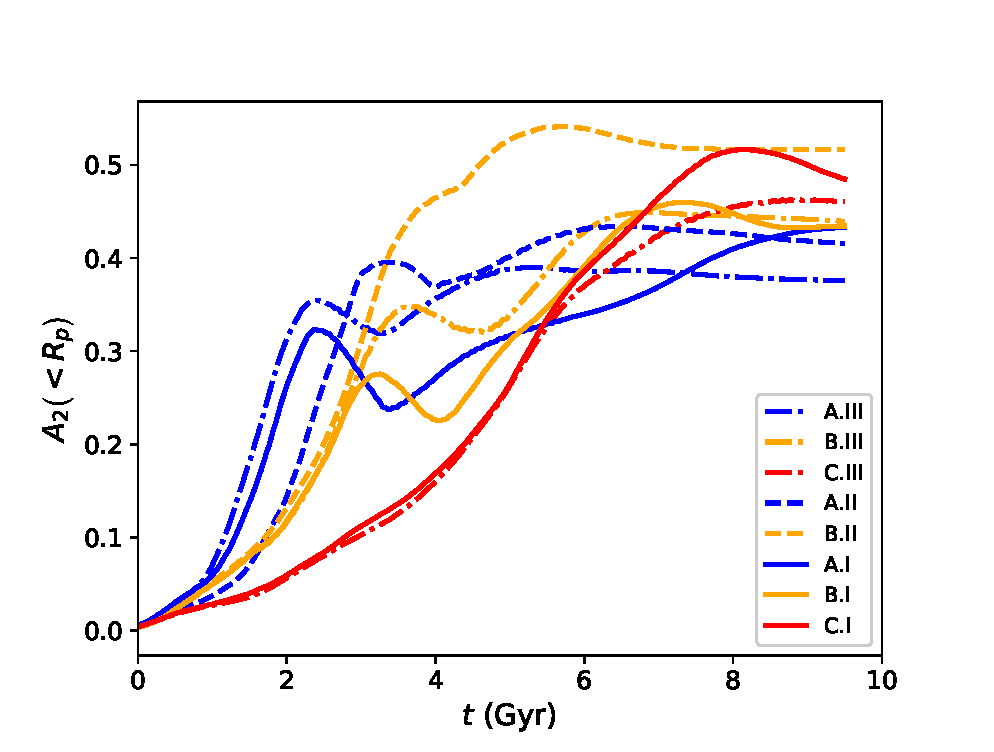
\includegraphics[width=0.8\textwidth]
{../figures/isolated_a2_vs_t_2rd_no_buckling_weighted.eps}
	\caption{Mean bar strength parameter inside the cylindrical
          radius $R_p$, $A_2(<R_p)$, as a function of time.  The
          figure is essentially the same as
          Fig.\,\ref{fig:isolated_a2_vs_t} though this time we include
          simulations A.III, B.III, and C.III where buckling is
          suppressed.} \label{fig:isolated_a2_vs_t_no_buckle}
\end{figure}


\begin{figure}
	\centering
	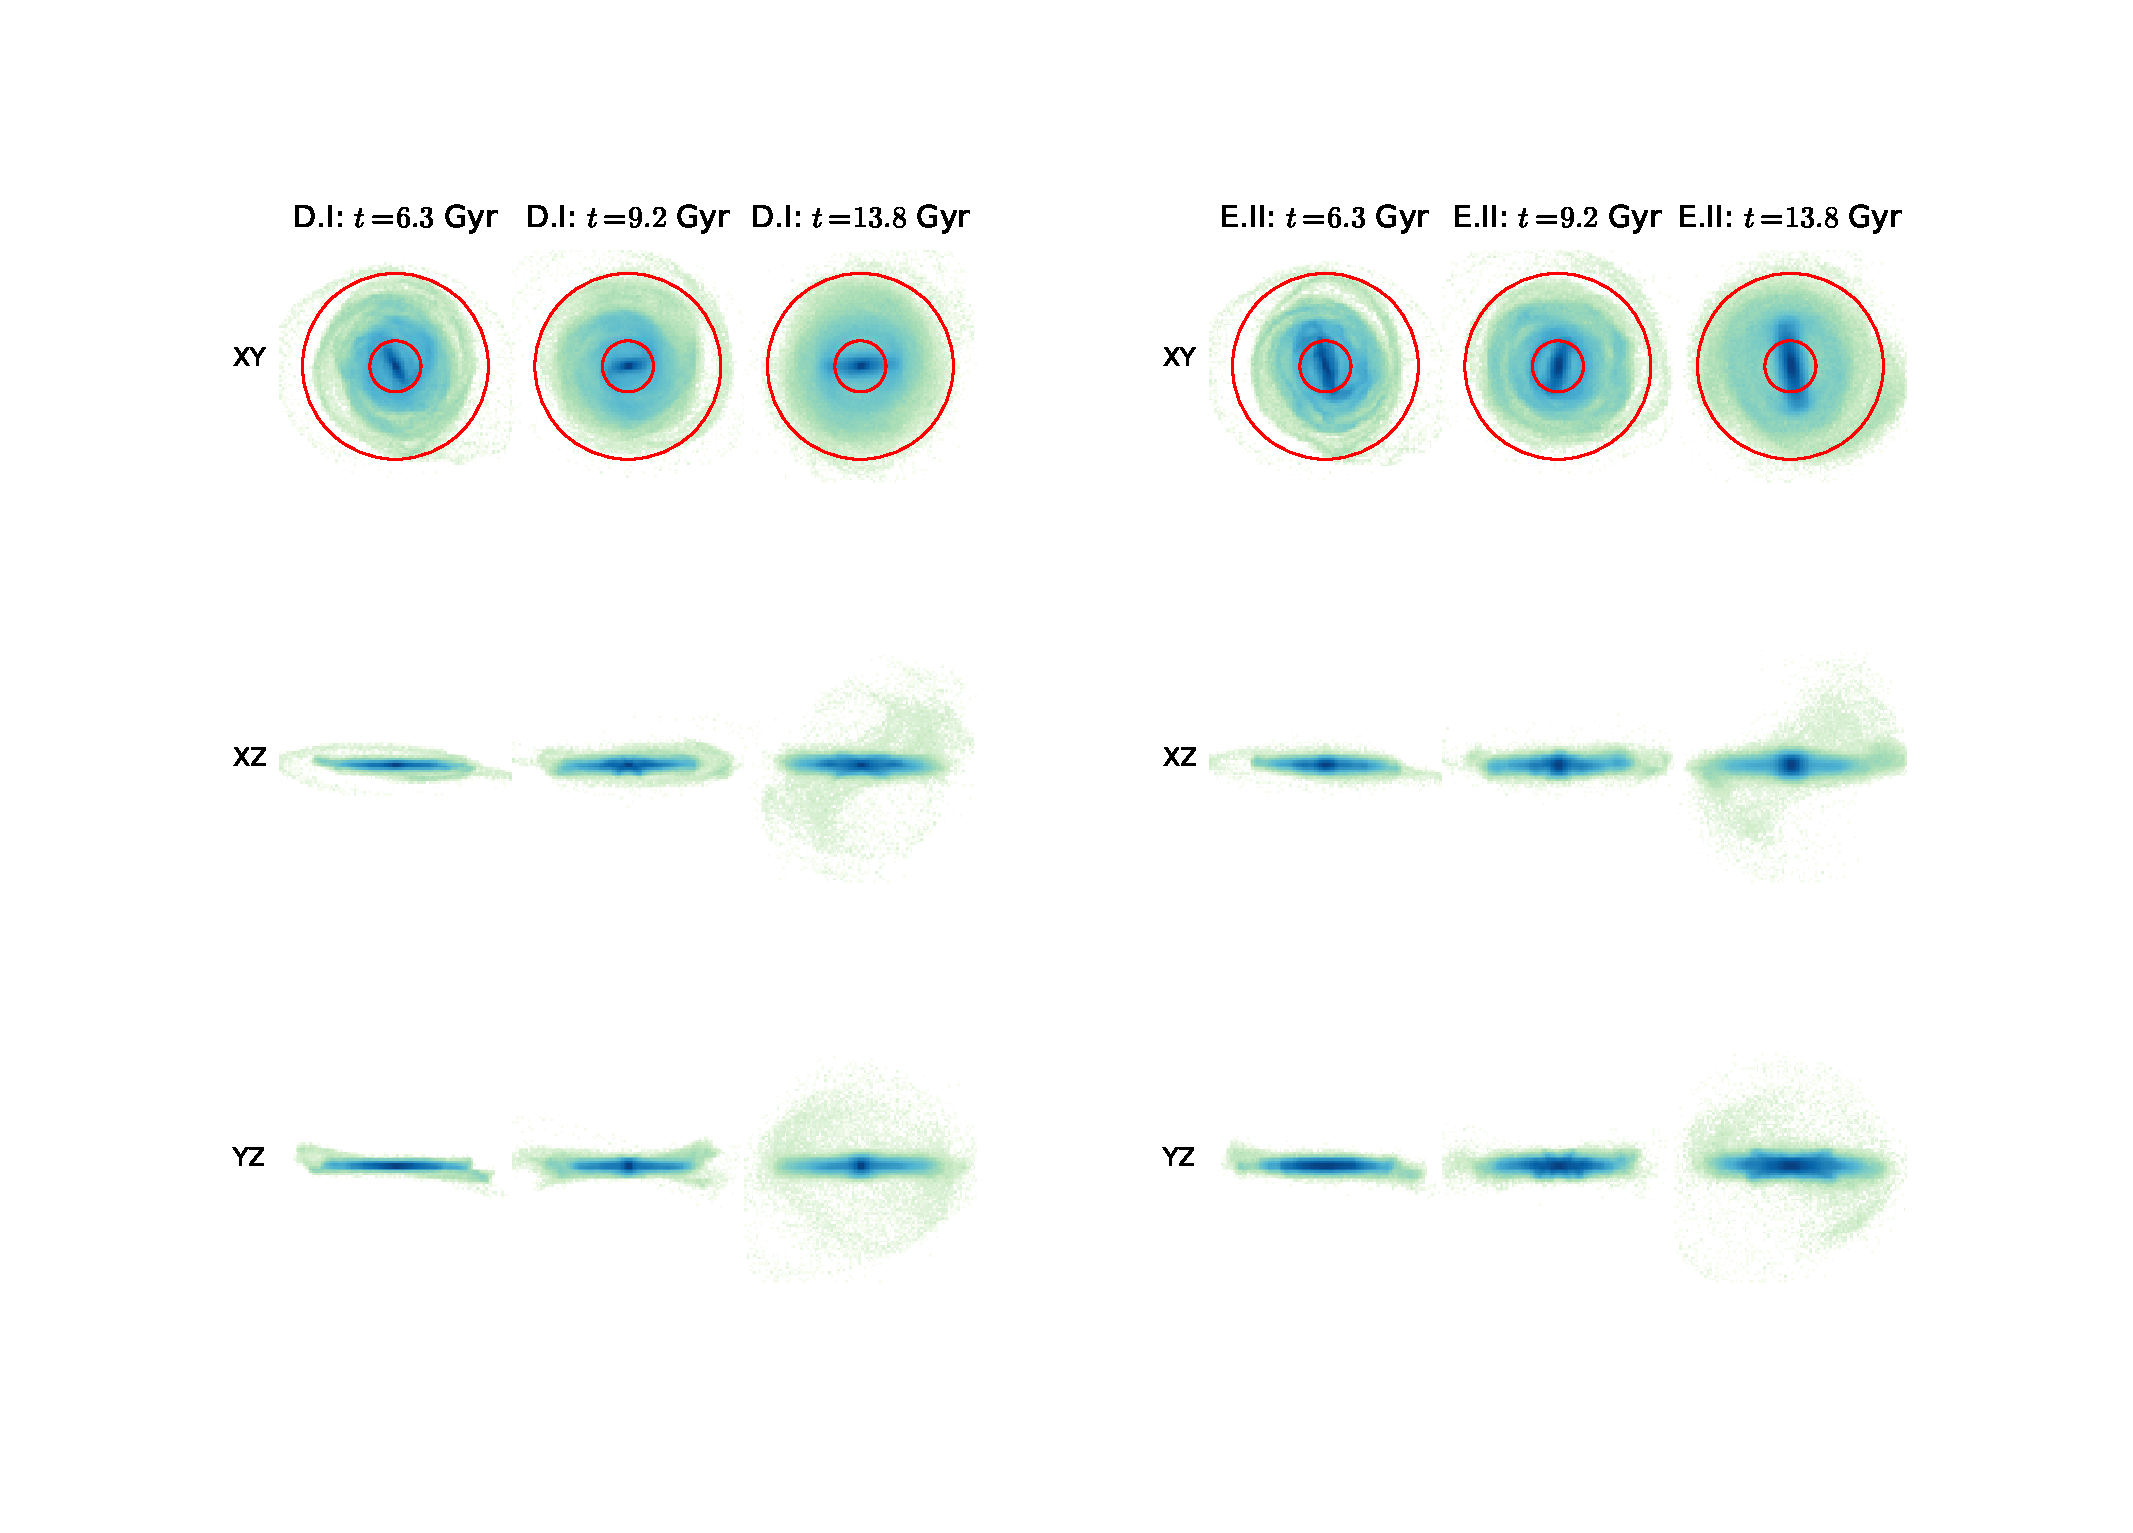
\includegraphics[width=\textwidth]{../figures/cosmo_three_by_threes.eps}
	\caption{Projections for the D.I (left three columns) and E.II
          (right three columns).  The three columns for each
          simulation correspond,from left to right, to $2.2\,{\rm
            Gyr}$, $5.9\,{\rm Gyr}$, and $13.7\,{\rm Gyr}$ after the
          Big Bang. The overlaid red circles have radii $R_p$ and 20
          $h^{-1} \,$kpc.} \label{fig:face_on_cosmo}
\end{figure}

\begin{figure}
	\centering
	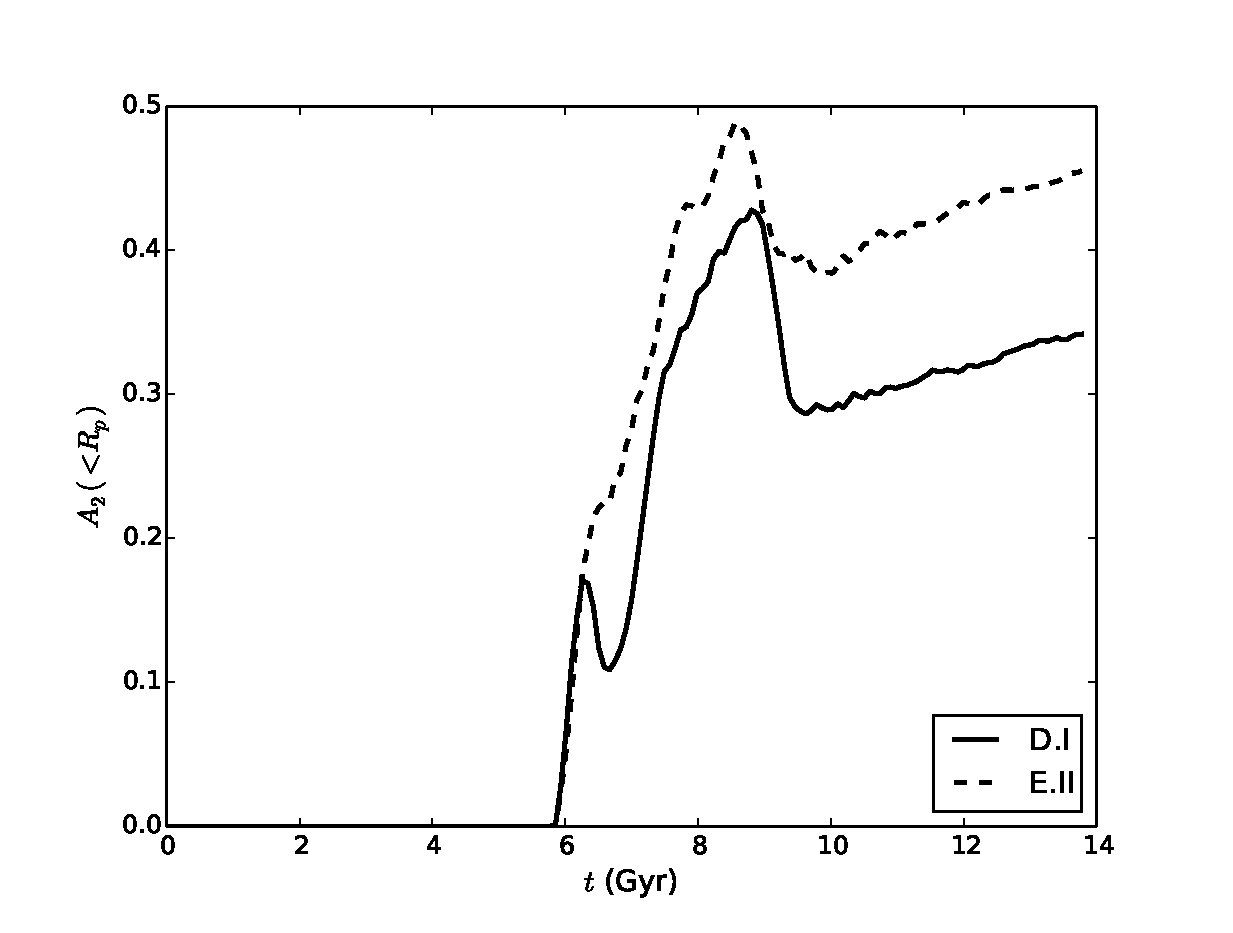
\includegraphics[width=0.8\textwidth]{../figures/cosmo_a2_vs_t_2rd_weighted.eps}
	\caption{$A_2(<R_p)$ as a function of the age of the Universe
          for simulations D.I (solid curve) and E.II (dashed
          curve). } \label{fig:cosmo_a2_vs_t}
\end{figure}


\begin{figure}
	\centering
	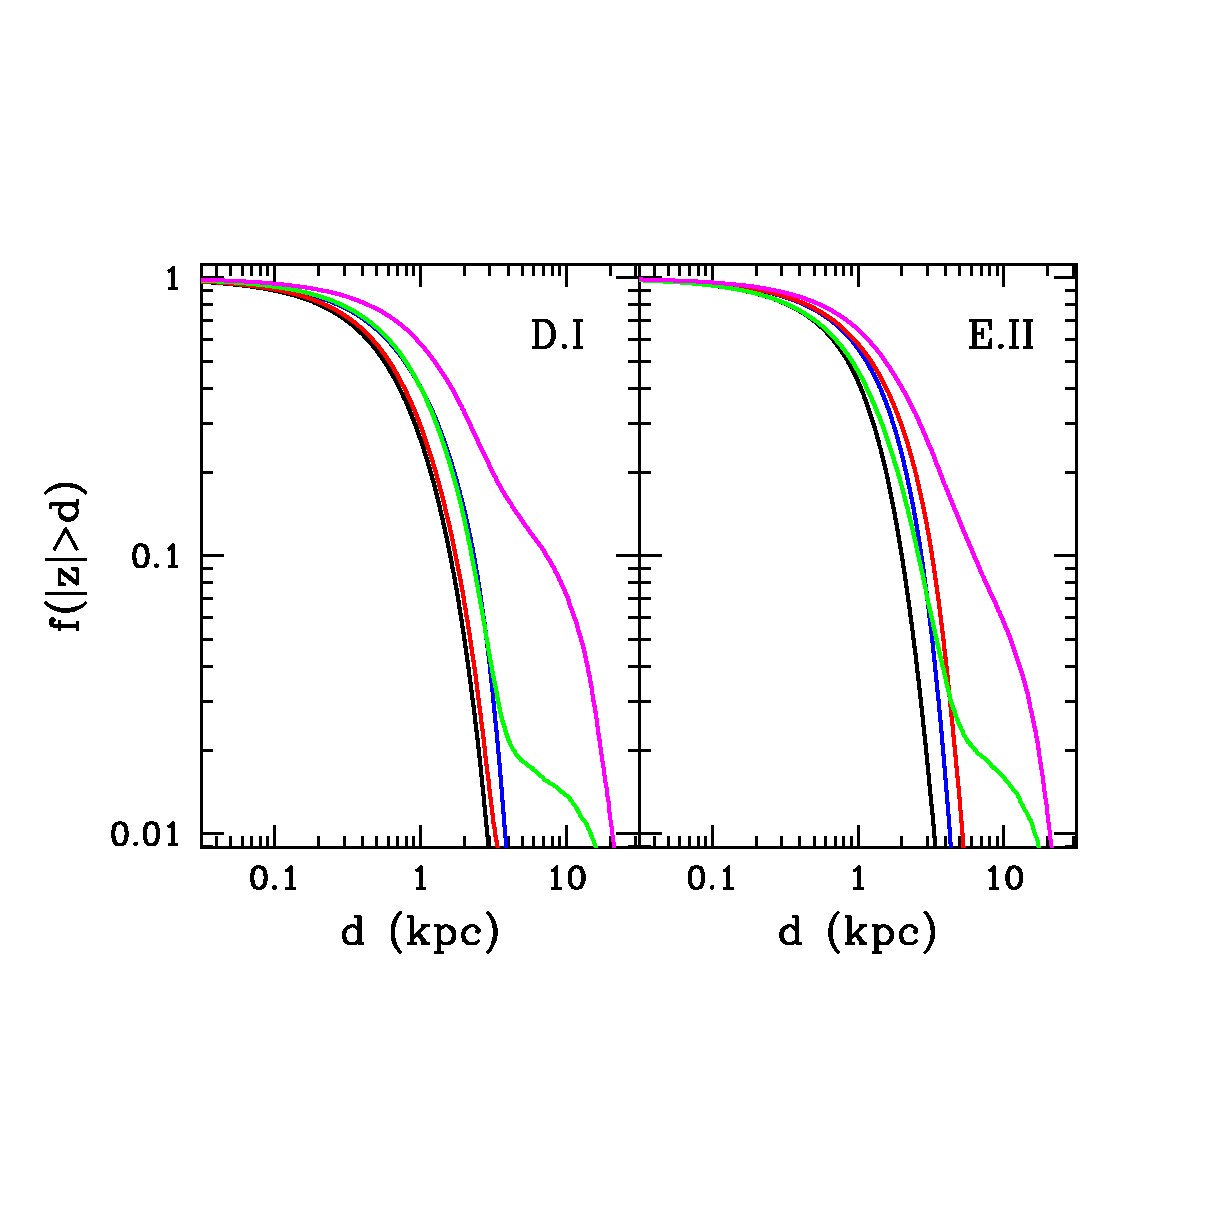
\includegraphics[width=0.8\textwidth]{../figures/kicked_up_disk.eps}
	\caption{Fraction of particles with distance from the midplane greater
than some distance $d$ as a function of $d$.  The difference colours correspond to
different bins in cylindrical radius $R$: $0<R<5\,{\rm kpc}$ --- black;
$5\,{\rm kpc} < R < 10\,{\rm kpc}$ --- blue;
$10\,{\rm kpc} < R < 15\,{\rm kpc}$ --- red;
$15\,{\rm kpc} < R < 20\,{\rm kpc}$ --- green;
$20\,{\rm kpc} < R\,{\rm kpc}$ --- magenta.}
 \label{fig:kicked_up_disc}
\end{figure}

\section{Cosmological Simulations} \label{sec:cosmo}

Disc galaxies simulated from axisymmetric, equilibrium initial
conditions, as was done in the previous section, form bars at rates
and with strengths that depend on their intrinsic scale height of the
disc and on the force resolution of the simulation. In this section,
we investigate the extent to which these results hold in a
cosmological environment.  In particular we follow the evolution of a
thin disc with moderate softening and a thick disc with high softening
that are embedded in identical cosmological haloes.

\subsection{Simulation Setup; Inserting Discs into Cosmological Haloes}

We model a stellar disc in a cosmological halo using the disc
insertion scheme described in \citet{Bauer2018a}.  This scheme, which
builds on the methods developed by
\citet{BerentzenShlosmanStellarDisks}, \citet{DeBuhrStellarDisks}, and
\citet{YurinSpringelStellarDisks} uses an iterative procedure to
initialize the disc.  The first step is to run a pure dark matter
simulation and identify a suitable halo.  The system is then rerun
from redshift $z_g$ to $z_l$, this time with a disc potential that
grows slowly in mass and radius.  Doing so allows the halo particles
to respond to the gravitational field of the would-be disc.  At $z_l$,
the rigid disc is replaced by an N-body system and the ``live'' disc-halo
system is evolved to the present epoch.

For our pure dark matter simulation, we implement the zoom-in
technique of \citet{KatzQuasarZoom} and \citet{NavarroWhiteZoom},
broadly following the recommendations of \cite{onorbe_etal_2014},
which allows us to achieve very high spatial and mass resolution for a
single halo while still accounting for the effects of large-scale
tidal fields.  We choose cosmological parameters based on the results
from Planck 2013 \citep{planck_2014} with $H_0=67.9\,{\rm
  km\,s}^{-1}\,{\rm kpc}^{-1}$, $\Omega_b = 0.0481$, $\Omega_0 =
0.306$, $\Omega_\Lambda = 0.694$, $\sigma_8 = 0.827$, and $n_s =
0.962$.  N-body initial conditions for the dark matter particles are
generated with the \textsc{music} code \citep{music}.  
We select a suitably-sized halo for a Milky Way-like galaxy, namely
one with a $z=0$ mass of $1.23\times 10^6\,h^{-1} M_\odot$
that comprises $10^6$.

During its growth phase from $z_g=3$ to $z_l=1$, the disc is treated
as a rigid body whose orientation and center-of-mass position evolve
according to the standard equations of rigid body dynamics.  At
$z_l$, we swap a live disc for the rigid one using the
\textsc{GalactICS} code
\citep{KGGalactICSReference,WPDGalactICSReference}, which generates a
three-integral DF disc in the best axisymmetric approximation to the
halo \citet{Bauer2018a}.

We run two simulations, D.I, which assumes a thin disc with a
softening length of $184\,{\rm pc}$ and E.II, which assumes a thick
disc with a softening length of $736\,{\rm pc}$.  The softening length
chosen for D.I is in accord with the criteria outlined in
\citet{power_et_al_2003}.  The simulations D.I and E.II roughly
correspond to A.I and B.II, respectively.  As well, E.II is similar to
the discs considered by \citet{DeBuhrStellarDisks},
\citet{YurinSpringelStellarDisks} and \citet{Bauer2018a}, whereas D.I
is more consistent with typical discs considered in isolated galaxy
suites like \citet{WPDGalactICSReference}.

\subsection{Results}

Results from our two cosmological simulations are displayed in
Figs.\,\ref{fig:face_on_cosmo} and \ref{fig:cosmo_a2_vs_t}.  The
former shows projections of the mass density at three epochs while the
latter gives $A_2(<R_p)$ as a function of time.  Evidently, the discs
in both cases roughly follow the same evolutionary sequence that was seen in
the isolated galaxy simulations: rapid growth of the bar strength
followed by a period where the bar strength decreases,
presumably due to buckling, and finally steady strengthening of the
bar.  The three epochs chosen in Fig.\,\ref{fig:face_on_cosmo}
correspond to the initial growth phase of the bar
($a=0.6,~t=6.3\,{\rm Gyr}$), an epoch after buckling
($a=0.7,~t = 9.2\,{\rm Gyr}$), and the present epoch at
$t=13.8\,{\rm Gyr}$.  Visually, the bar appears to be stronger and
longer in the E.II run than D.I one at each of these epochs but
perhaps most notably in the final one.  Indeed, the disc in E.II looks
very similar to those seen in the simulations of
\citet{DeBuhrStellarDisks}, \citet{YurinSpringelStellarDisks}, and
\citet{Bauer2018a}.  The fact that the bar in D.I is weaker than the
one in E.II is consistent with the results from our isolated galaxy
simulations that thicker discs produce stronger bars (see
Fig.\,\ref{fig:face_on_isolated}).

The most significant difference between bar formation in the
cosmological setting and bar formation in isolated galaxies concerns
the initial growth of the bar.  For isolated galaxies,
Fig.\,\ref{fig:isolated_a2_vs_t} clearly shows that the onset of bar
formation is delayed for thicker discs.  Conversely, in the
cosmological case, $A_2$ rapidly grows to a value of $\sim 0.17$
within the first few hundred Myr after the disc ``goes live''
regardless of the disc thickness.  At this point, the bar in the thin
disc model decreases in strength with $A_2$ dropping to $\sim 0.11$
before resuming its growth.  By contrast, the bar in the thick disc
model continues to grow monotonically.  As in the isolated galaxy
simulations, self-regulating processes such as buckling are more
efficient in the thin disc case and so $A_2$ in simulation D.I lags
behind that of E.II.  We note that in both cases, $A_2$ drops
significantly at around $t=7.5\,{\rm Gyr}$ and grows steadily
thereafter.

Our interpretation of these results is as follows: In isolation, where
discs start from axisymmetric initial conditions, the only source of
the $m=2$ perturbations that drive bar formation is shot noise from
the N-body distribution.  Evidently, making a disc thicker slows the
growth of these perturbations.  On the other hand, $m=2$ perturbations
abound in the cosmological environment where haloes are clumpy and
triaxial.  The initial growth of the bar may, in fact, be relatively
insensitive to the thickness of the disc, once discs are placed in a
cosmological setting.  On the other hand, disc thickness does effect
the resilience of the bar to self-regulating processes, such that
buckling and therefore thick discs tend to have stronger bars.

Finally, we note that in both D.I and E.II, a significant number of
particles are found at high galactic latitudes.  These particles
represent stars ``kicked-up'' from the disc presumably by the
large-scale tidal fields of the halo and interactions between the disc
and halo substructure.  Kicked-up stars have been seen in cosmological
simulations by \citet{purcell2010}, \citet{mccarthy2012} and
\citet{tissera2013}.  Their existence was inferred in a combined
analysis of kinematic and photometric data for the Andromeda galaxy
\citep{dorman2013}.  Furthermore, the idea of kicked-up stars has been
invoked by \citep{pricewhelan2015} to explain the Triangulum-Andromeda
stellar clouds \citep{rochapinto2003, martin2014} and by
\citep{sheffield2018, laporte_2018_low_latitude} to explain the Monoceros Ring \citep{yanny2000,
  newberg_2002} and associated A13 stellar overdensity
\citep{sharma2010}.

In Fig.\,\ref{fig:kicked_up_disc} we show the fraction of stars with
$|z|>d$ for different regions of the discs in our two cosmological
simulations.  The results are strikingly similar for the two
simulations as is already evident from a visual inspection of 
Fig.\,\ref{fig:face_on_cosmo}. The implication is that
the processes by which stellar orbits are
perturbed out of the disc plane are relatively insensitive to the
vertical structure of the disc.  We see that very few of the stars
with cylindrical radius $R<15\,{\rm kpc}$ and only $1-2\,\%$ of the
stars between $15$ and $20\,{\rm kpc}$ are kicked-up to distances
greater than $3\,{\rm kpc}$ though some stars from the $15-20\,{\rm
  kpc}$ region do end up with $|z|> 10\,{\rm kpc}$.  On the other
hand, $20\,\%$ of the stars from the region beyond $20\,{\rm kpc}$ end
up with $|z|> 3\,{\rm kpc}$ from the midplane and $10\,%$ end up $|z|>
10\,{\rm kpc}$.  Of course, the actual number of stars is certainly
larger since a fraction of the kicked-up stars will be passing through
the disc with large vertical velocities.

\section{Conclusions}\label{sec:conclusions}
{
We briefly summarize our findings as:
\begin{itemize}
\item Bar strength in a cosmological setting depends on $X$ and $Q$, as well as additional properties such as thickness and vertical dispersion.
\item In isolation, thick discs appear more resilient to buckling.
\item In a cosmological setting, environment appears to be a much larger driver of bar formation than internal disc dynamics.
\item Disc scale height has little-to-no impact on the number of stars being kicked out of a stellar disc.
\end{itemize}
}

The seminal work of \citet{PeeblesOstriker1973} introduced the notion
that disc dynamics provides a powerful constraint on the structure of
discs and the haloes in which they reside.  In short, discs that are
dynamically cold and that account for a substantial fraction of the
gravitational force that keeps their stars on nearly circular orbits
are unstable to the formation of strong bars and spiral structure.
The existence of galaxies with weak bars or no bars at all tells us
that at least some discs are relatively low in mass (i.e., submaximal)
and/or dynamically warm.

The theoretical analysis presented in Section 2 showed with a few
simple assumptions (e.g., exponential surface density profile) one can
derive a relation among the structural parameters of a disc in
approximate equilibrium and thus a constraint on initial conditions
that one might choose for simulations.  For example, if one fixes
$z_d/R_d$ and $\sigma_R/\sigma_z$, as was done in
\citet{YurinSpringelStellarDisks}, then there is an approximately
one-to-one relationship between $Q$ and $X$.  Likewise, fixing $Q$ and
$X$ implies a relationship between $z_d/R_d$ and $\sigma_R/\sigma_z$.
These results have important implications for applying disc dynamics
as a constraint on models of galaxy formation.  In particular,
inconsistencies between bar demographics in a galaxy formation model
and in observational surveys may reflect differences in the scale
height and vertical velocity dispersion of model and real galaxies.

One lesson from our work and the work of others is that the relation
between structural parameters of galaxies and bar strength and length
is often rather complicated.  This observation is no doubt due, at
least in part, to the self-regulating nature of bar formation.  When
bars develop rapidly, they tend to buckle, which leads to weaker and
shorter bars \citep{VP2004}.  Thick discs appear to be more resilient
to buckling, which may explain why bars in these models often end up
stronger and longer than bars in thin-disc models \citep{Klypin2009}.
For similar reasons, gravitational softening can affect the
development and ultimate strength of bars.

In simulations of isolated galaxies from ``pristine'' equilibrium
initial conditions, bar formation is seeded by the shot noise of the
N-body distribution.  On the other hand, bars in a cosmological
environment are subjected to large perturbations including the $m=2$
ones that drive bar formation.  Thus, the fact that bar formation is
delayed in thick disc models of isolated galaxies may be purely
academic --- bar formation in the cosmological environment will be
initiated by a variety of stochastic effects regardless of the
thickness of the disc.  On the other hand, the resilience of thick
discs to buckling {\it is} relevant in the cosmological setting and
may explain why thick discs tend to form strong bars.  The upshot is 
that a proper understanding the distribution of bars in cosmological models
must go hand-in-hand with a proper understanding of the vertical 
structure of discs.

Clearly, a more exhaustive exploration of the model parameter space is
in order.  One might, for example, include galaxy scaling relations to
further constrain the space of models.  In addition, it would be of
interest to insert different discs (and for that matter, nearly
identical ones) into different haloes in order to explore the
random nature of disc-halo interactions.  Ultimately, improvements
in observations together with a more complete survey of models via
simulations should allow us to fully exploit bars in discs as a means
of testing and constraining theories of structure formation.

\section*{Acknowledgements}
{LMW and JSB are supported by a Discovery Grant with the Natural
  Sciences and Engineering Research Council of Canada. JSB
  acknowledges the assistance of Matthew Chequers and Keir Darling in
  understanding the \textsc{AGAMA} program interface. The authors
  acknowledge the contributions of the Python scientific open source community,
  particularly the SciPy project \citep{scipy}, NumPy \citep{numpy}, Pandas \citep{pandas},
  and matplotlib \citep{matplotlib}.}

%%%%%%%%%%%%%%%%%%%%%%%%%%%%%%%%%%%%%%%%%%%%%%%%%%

%%%%%%%%%%%%%%%%%%%% REFERENCES %%%%%%%%%%%%%%%%%%

% The best way to enter references is to use BibTeX:

\bibliographystyle{apalike}
\bibliography{bibliography_paper_ii.bib} % if your bibtex file is called example.bib
\chapter{Forming Vertical Structure in $\Lambda$CDM Discs}\label{ch:paper_iii}

%\include{Alloy}

%\include{Embee_UserPerspective}
%\include{Embee_Implementation}

\chapter{Summary and Conclusions}\label{ch:Conclusion}

In this chapter, we summarize the  main findings of this thesis and talk about future work.


\section{Interactions Between Stellar Disks and Dark Matter Halos}


\subsection{Summary}

One of the key contributions of this thesis is the understanding of how the dynamic nature of stellar disks affects halo properties. Although the material in Chapter~\ref{ch:paper_i} is primarily focused on introducing a method used by our group, its key scientific contributions focus on this point.

We found that modelling the disk in a dynamic fashion is tremendously important for the inner halo. Specifically, we found the formation of a bar led to a more concentrated halo mass distribution.

The intermediate-to-outer halo was less effected by the dynamics of the inner halo. While some differences between our disk potential models were observed in the halo mass functions, these differences were minor. The details of how satellites are disrupted appear to be at least weakly dependent on how the disk is modelled, and stream studies should consider as realistic of a disk as possible.

\subsection{Future Work}

\section{Bar Formation in Cosmological Stellar Disks}
\subsection{Summary}

\subsection{Future Work}
\section{Vetical Structure in Cosmological Stellar Disks}

%*************************************************************************************************************
% BIBLIOGRAPHY
%*************************************************************************************************************
% This GATHER command is useful for when you want to use WinEdt's Gather functionality, i.e., type
% \cite{} and a popup box appears with all of your citations to choose from.  Leave the % on the next line.
%GATHER{thesis.bib}

% Put in \nocite{*} so all entries in the bibliography are included
%\nocite{*}

%\bibliographystyle{apalike}
%\bibliography{../bibliography.bib}
\appendix

\definecolor{codegreen}{rgb}{0,0.6,0}
\definecolor{codegray}{rgb}{0.5,0.5,0.5}
\definecolor{codepurple}{rgb}{0.58,0,0.82}
\definecolor{backcolour}{rgb}{0.95,0.95,0.92}


\chapter{Referenced Code: kicks.c} \label{ch:kicks.c}
\lstinputlisting[language=C,basicstyle=\footnotesize,
    commentstyle=\color{codegreen},
    keywordstyle=\color{magenta},
    numberstyle=\tiny\color{codegray},
    stringstyle=\color{codepurple},]{kicks.c}]

\chapter{Referenced Code: predict.c} \label{ch:predict.c}
\lstinputlisting[language=C,basicstyle=\footnotesize,
    commentstyle=\color{codegreen},
    keywordstyle=\color{magenta},
    numberstyle=\tiny\color{codegray},
    stringstyle=\color{codepurple}]{predict.c}]


\chapter{Referenced Code: extract\_halo\_ascii.py} \label{ch:extract_halo_ascii.py}
\lstinputlisting[language=Python,basicstyle=\footnotesize,
    commentstyle=\color{codegreen},
    keywordstyle=\color{magenta},
    numberstyle=\tiny\color{codegray},
    stringstyle=\color{codepurple},]{extract_halo_ascii.py}]
    
    
\chapter{Referenced Code: merge\_ics.cpp} \label{ch:merge_ics.cpp}
\lstinputlisting[language=C++,basicstyle=\footnotesize,
    commentstyle=\color{codegreen},
    keywordstyle=\color{magenta},
    numberstyle=\tiny\color{codegray},
    stringstyle=\color{codepurple},]{merge_ics.cpp}]
    
\chapter{Referenced Code: timestep.c} \label{ch:timestep.c}
\lstinputlisting[language=C,basicstyle=\footnotesize,
    commentstyle=\color{codegreen},
    keywordstyle=\color{magenta},
    numberstyle=\tiny\color{codegray},
    stringstyle=\color{codepurple},]{timestep.c}]

%*************************************************************************************************************
% APPENDICES
%*************************************************************************************************************
\updatechaptername
%\appendixpage
\appendix

%\include{App_AnalyzerCode}
%\include{App_ExtraAnalysis}
%\addappheadtotoc

%*************************************************************************************************************
% GLOSSARY
% Using a glossary is more than beginners need to know; leaving the packages, etc. here for now.
%*************************************************************************************************************
%\usepackage[nonumberlist]{glossaries}
%\usepackage[refpages]{gloss}  % for my glossary
                              % refpages shows the first page where the term occurs
%-------------------------------------------------------------------------------------------------------------
% Tell Latex to make a glossary
%*************************************************************************************************************
%\makeglossaries  % tell latex to make the glossary
%\glossarystyle{list}

%*************************************************************************************************************
% INDEX
%*************************************************************************************************************
% Here's where the index would be printed, if you created one.  Remove the % on the next line.
%\printindex


%*************************************************************************************************************
\end{document}
